\documentclass[12pt,Bold,TexShade]{mcgilletdclass}
\usepackage[pdftex]{graphicx}
\usepackage{subfig}
\usepackage{algpseudocode}
\usepackage{algorithm}
\usepackage{listings}
\usepackage{color}
\usepackage[labelformat=simple]{caption}
\usepackage[dvips]{geometry}
\usepackage{amsmath}
\DeclareMathOperator*{\argmax}{argmax}
\DeclareMathOperator*{\argmin}{argmin}
\usepackage{amssymb}
\usepackage{url}
\usepackage{siunitx}
\usepackage{appendix}
\usepackage{hyperref}
\usepackage{natbib}

\usepackage{todonotes}

% \renewcommand\thesubfigure{\alph{subfigure})}
%%%%%%%%%%%%%%%%%%%%%%%%%%%%%%%%%%%%%%%%%%%%%%%%%%%%%
%% Have you configured your TeX system for proper  %%
%% page alignment? See the McGillETD documentation %%
%% for two methods that can be used to control     %%
%% page alignment. One method is demonstrated      %%
%% below. See documentation and the ufalign.tex    %%
%% file for instructions on how to adjust these    %%
%% parameters.                                     %%
\addtolength{\hoffset}{0pt}                        %%
\addtolength{\voffset}{0pt}                        %%
%%                                                 %%
%%%%%%%%%%%%%%%%%%%%%%%%%%%%%%%%%%%%%%%%%%%%%%%%%%%%%
%%       Define student-specific info
\SetTitle{\huge{Unsupervised Learning of Interpretable Models for Sparse, Smooth Data}}%
\SetAuthor{Arnold Kalmbach}%
\SetDegreeType{Master of Computer Science (Thesis)}%
\SetDepartment{Department of Computer Science}%
\SetUniversity{McGill University}%
\SetUniversityAddr{Montreal, Quebec}%
\SetThesisDate{\today}%
\SetRequirements{A thesis submitted to McGill University in partial fulfillment of requirements for
the degree of Master of Computer Science}%
\SetCopyright{\copyright{Arnold Kalmbach, 2018}}%

% \makeindex[keylist]
% \makeindex[abbr]

%% Input any special commands below
%\newcommand{\Kron}[1]{\ensuremath{\delta_{K}\left(#1\right)}}
\listfiles%
\begin{document}

\maketitle%

\begin{romanPagenumber}{2}%
\SetDedicationName{DEDICATION}%
\SetDedicationText{This thesis is dedicated to my teachers throughout the years, inside and outside classrooms, foremost to my parents Faye and Arnold, and to my sister Ilana.}%
\Dedication%

\SetAcknowledgeName{ACKNOWLEDGEMENTS}%
\SetAcknowledgeText{\vspace{-12pt} Studying at McGill has been an incredible journey and a great priviledge, and I would like to thank everyone who made my time here as memorable as it was illuminating. Foremost, I would like to thank my supervisor Gregory Dudek for his guidance, encouragement, and infectious enthusiasm for interesting ideas. I also would like to express my gratitude for labmate, mentor and friend, Yogesh Girdhar, whose work is the starting point of this thesis, and whose own adventures led me to an extremely rewarding semester abroad at Woods Hole Oceangraphic Institution. I'd also like to thank all of the members of the Mobile Robotics Lab; Florian, Juan, Sandeep, Travis, Jimmy, Nikhil, Andrew, Johanna, Lucas, Wei-Di, Karim, Monica, Ed, Scott, Anqi, Malika, Isabelle, Yiannis, Yogi, Dave, and Greg, for building a vibrant, energizing community, and for fruitful collaborations and valuable feedback throughout my studies. I'd like to express extra gratitude to Florian and Juan, for being extra dependable friends and sources of good advice, as well as to Wei-Di, for all his help in our active vision experiments over the past year. Thanks also go to my friends outside the lab, Steve, Brian, Matt, and Ben, who helped keep my work connected to the world at large, and who enrich my perspective and my life. Finally, I'd like to thank my family: my partner, Katie (who helps keep me sane every single day), my mother, Faye, my father, Arnold, and my sister Ilana; For their unconditional support and caring, no matter how many times I tried out unfinished, incomprehensible explanations of my work on them.}%
\Acknowledge%

%%%%%%%%%%%%%%%%%%%%%%%%%%%%%%%%%%%%%%%%%%%%%%%%%%%%%
%%         English Abstract                        %%
%%%%%%%%%%%%%%%%%%%%%%%%%%%%%%%%%%%%%%%%%%%%%%%%%%%%%
\SetAbstractEnName{ABSTRACT}%
\SetAbstractEnText{
% \todo{Are you sure "maps" is the right term for the abstract?  As opposed to either "mappings", or "image manifolds",m or "sensorial maps", or maybe "image mappings"?}
This thesis considers learning unsupervised representations that facilitate understanding how complex data varies over space and time -- in other words learning interpretable semantic spatio-temporal maps. We focus on representations that are \emph{sparse}, meaning most locations are described by few types, and \emph{smooth}, meaning most locations are described by the same types as their neighbors. We investigate how a spatio-temporal topic model -- a descendent of Latent Dirichlet Allocation (LDA) and other probabilistic latent variable models -- can be used to learn such representations for problems outside the typical text domain associated with LDA. We apply spatio-temporal topic models to a broad range of domains including modelling ambient audio, phytoplankton populations, and images observed by a robotic camera. In developing this variety of applications, we introduce novel interpretations of the learned topic model; beyond simple clustering or unsupervised classification we also consider using the topic model to make predictions in feature space and in the space of raw observations. In our experiments we demonstrate that sparse and smooth map representations are more interpretable than alternative unsupervised representations. We evaluate this interpretability in terms of both alignment with natural human-centric representations as well as the ease of learning later supervised models.
}
\AbstractEn%

%%%%%%%%%%%%%%%%%%%%%%%%%%%%%%%%%%%%%%%%%%%%%%%%%%%%%
%%         French Abstract                         %%
%%%%%%%%%%%%%%%%%%%%%%%%%%%%%%%%%%%%%%%%%%%%%%%%%%%%%
\SetAbstractFrName{ABR\'{E}G\'{E}}%
\SetAbstractFrText{\vspace{-20pt} Cette th\`{e}se consid\`{e}re l'apprentissage des repr\'{e}sentations non supervis\'{e}es qui facilitent la compr\'{e}hension de la variation des donn\'{e}es complexes dans l'espace et dans le temps, c'est-\'{a}-dire l'apprentissage des cartes spatio-temporelles s\'{e}mantiques interpr\'{e}tables. Nous nous concentrons sur les repr\'{e}sentations qui sont \emph{clairsem\'{e}es}, ce qui signifie que la plupart des endroits sont d\'{e}crits par quelques types, et \emph{r\'{e}guli\`{e}res}, ce qui signifie que la plupart des endroits sont d\'{e}crits par les m\^{e}mes types que leurs voisins. Nous \'{e}tudions comment un mod\`{e}le th\`{e}matique spatio-temporel ('spatio-temporal topic model') - un descendant de `Latent Dirichlet Allocation' (LDA) et d'autres mod\`{e}les de variables latentes probabilistes - peut \^{e}tre utilis\'{e} pour apprendre de telles repr\'{e}sentations pour des probl\`{e}mes ext\'{e}rieurs du domaine de texte associ\'{e} \`{a} LDA. Nous appliquons des mod\`{e}les th\`{e}matiques spatio-temporels \`{a} une large gamme de domaines, y compris la mod\'{e}lisation de l'audio ambiant, des populations de phytoplancton et des images observ\'{e}es par une cam\'{e}ra robotis\'{e}e. En d\'{e}veloppant cette vari\'{e}t\'{e} d'applications, nous introduisons de nouvelles interpr\'{e}tations du mod\`{e}le th\`{e}matique appris; plus que du simple regroupement ou de la classification non supervis\'{e}e, nous envisageons \'{e}galement d'utiliser le mod\`{e}le th\`{e}matique pour faire des pr\'{e}dictions dans l'espace objet et dans l'espace des observations propres. Dans nos essais, nous d\'{e}montrons que les repr\'{e}sentations de carte clairsem\'{e}es et lisses sont plus interpr\'{e}tables que les repr\'{e}sentations standards non supervis\'{e}es. Nous \'{e}valuons cette interpr\'{e}tabilit\'{e} en relation avec l'alignement avec les repr\'{e}sentations naturelles centr\'{e}es sur l'homme et aussi la facilit\'{e} d'apprentissage des mod\`{e}les supervis\'{e}s bas\'{e}s sur nos repr\'{e}sentations.}%
\AbstractFr%

\TOCHeading{TABLE OF CONTENTS}%
\LOTHeading{LIST OF TABLES}%
\LOFHeading{LIST OF FIGURES}%

\tableofcontents %
\listoftables %
\listoffigures %

\begin{center}
LIST OF SYMBOLS\\
\begin{tabular}{cp{\textwidth}}
  $x$ & Location, spatial or spatio-temporal \\
  $w$ & Word, an instance of a discrete-valued feature ($\textbf{w}$, all words) \\
  $z$ & Topic assignment ($\textbf{z}$, all topic assignments) \\
  $g(x)$ & The neighborhood of location $x$ \\
  $g$ & Parameter controlling neighborhood size \\
  $\theta$, $\theta_{g(x)}$ & Topic prior for one neighborhood ($\Theta$, all topic priors)\\
  $\phi$, $\phi_k$ & Word distribution for one topic ($\Phi$, all topics) \\
  $\alpha$ & Parameter of symmetric Dirichlet prior on $\theta$ \\
  $\beta$ & Parameter of symmetric Dirichlet prior on $\phi$ \\
  $K$ & Number of topics \\
  $V$ & Vocabulary size, number of distinct values of $w$ \\
  $N_{g(x)}^k$ & Number of times topic $k$ was used in neighborhood $g(x)$ \\
  $N_k^v$ & Number of times topic $k$ was used for word $v$ \\
  $N_{\cdot,-i}^\cdot$ & Count as above, but excluding the $i$-th datapoint\\
  $\sigma$ & The softmax function where the $i$-th dimension $\sigma(x)_i = {e^{x_i}} / \sum_j e^{x_j}$ \\
  $H[X]$ & Entropy of the random variable $X$: \\
         & $\mathbb{E}[-\log P(x)]$ \\
  $D_{KL}[P,Q]$ & KL-Divergence (information gain) of PMFs $P, Q$:\\
         & $\mathbb{E}_X \left[\log P(x) - \log Q(x) \right]$ \\
  $MI[X,Y]$ & Mutual information between random variables $X, Y$:\\
         & $\mathbb{E}_X \left[\mathbb{E}_Y \left[P(x,y) \log\left(\frac{P(x,y)}{P(x)P(y)}\right) \right] \right]$
\end{tabular}
\end{center}

\end{romanPagenumber} 

\mainmatter %
%!TEX root = thesis.tex
\chapter{Introduction} \label{ch:intro}

\section{Context}
A fundamental goal of machine learning is to generate useful representations of rich, high-dimensional datasets, simplifying human understanding by learning to transform data.
In many cases, pairs of inputs and desirable outputs are available for training, leading to techniques and representations directly equipped with external meaning by imitation. However in many other cases the desireable outputs are unavailable; For example, when a robot explores a new type of environment for the first time, when a scientist is encountered with a new type of data, or when one algorithm is presented with a novel learned representation produced by another algorithm (all examples discussed in detail within this thesis).

Unsupervised learning is an area of machine learning that aims to address this lack of training labels. Classic methods include Principal Component Analysis (PCA) and k-means clustering, and are both efficient to train and relatively straightforward to interpret. Unfortunately, these approaches are too simplistic to capture natural categories in data such as images, text documents or audio that are most prevalent and interesting in human-oriented applications. PCA simply learns a linear projection based on the eigenvectors of the training data, i.e. a basis for the directions of greatest variance, while k-means just clusters data-points by approximately minimizing the distance to cluster centers. Neither method is able to capture the real-world complexity of most interesting datasets.

In contrast more recent unsupervised learning techniques employ deep neural networks (DNNs) to define more expressive unsupervised models; Restricted Boltzmann Machines (RBMs), autoencoders, and Generative Adversarial Networks (GANs) are model families of particular note for impressive performance on large-scale unsupervised learning tasks with real data \citep{Bengio2013,Goodfellow2014}. In general, these approaches use a sequence of non-linear activations trained by stochastic gradient descent to find a low dimensional representation of the data which preserves as much information about it as possible. Such `representation learning' techniques have been shown to be powerful as early computation stages for later supervised learning tasks. However, these supervised tasks are typically solved with complex models (often another DNN) rather than simple ones. Although these methods achieve impressive performance in an absolute sense, the representations themselves are opaque and resist human interpretation. Even when regularization steps are added, the significance of a feature dimension with respect to a `semantic dimension' is rarely natural.

A final group of unsupervised learning techniques are those that are deliberately constructed as Bayesian probabilistic graphical models (PGMs). These models take the data $\textbf{x}$ and hypothesize related hidden variables $\textbf{z}$ used as the learned representation, along with a joint distribution that factors into a conditional likelihood and a prior, $P(\textbf{x}, \textbf{z}) = P(\textbf{x}|\textbf{z}) P(\textbf{z})$. The representation for a data point is produced by posterior inference, for example choosing $z = \argmax_z P(z | x)$. This group is not mutually exclusive with the previous two: PCA can be interpreted as a PGM with a single latent multivariate normal variable \citep{Bishop1999}, k-means can be interpreted as PGM by its equivalence to a special case of the well-known Gaussian Mixture Model  \citep{BishopCh9}, and autoencoders with a particular form can be trained for approximate posterior inference with particular choices of likelihood and prior \citep{Kingma2014}. The essential feature of the Bayesian graphical model formalism is that it provides a mechanism to control the types of representations we would like to obtain without hard constraints, allowing models to take advantage of both weak domain knowledge and very general priors on the kinds of representations that can be easily interpreted.

\section{Scope}
In this thesis we consider Bayesian unsupervised learning for spatial, temporal, or spatio-temporal data, in other words, for a dataset lacking associated labels but with associated locations. We hypothesize that by choosing an appropriate prior we can learn to represent data in ways that are accurate without sacrificing interpretability. In particular, our work centers on Realtime Online Spatio-temporal Topic models (ROST) \citep{Girdhar2014}, a descendant of Latent Dirichlet Allocation (LDA) \citep{Blei2003} which favors representations that are simple and spatio-temporally smooth. In Ch.~\ref{ch:topic-models-detail} we provide a comprehensive review of the spatio-temporal topic model.

Using the spatio-temporal topic model, we address learning unsupervised representations of spatio-temporal data that are compatible with simple downstream learning tasks and human interpretations. We hypothesize that if raw data is transformed by an appropriate feature function and modeled with our approach, the representation learned by the spatio-temporal topic model can be aligned with human labels using a simple matching scheme. In addition, we consider scenarios where there are no manually-generated labels whatsoever and consider how the topic model may be used to gain intuitive insight into the factors that affect the data in the feature and raw data domains directly.

\section{Motivation}
The introduction of cheap commercial GPS receivers and improvements in inertial and visual state estimation has resulted in an ever expanding set of data sources which come with associated spatial data. In the context of robotics, in addition to classic obstacle based landmark and occupancy maps, it is advantageous for a robot to have a qualitative sense of what kind of place it is in. For instance it would be prudent for a flying robot to recognize whether it is over park, industrial, or residential land and modify its behavior for the appropriate balance of caution and efficiency. Nevertheless, these types of land may appear vastly different in different regions and with different cameras (or completely distinct sensor modalities), therefore a robot should be able to learn to differentiate between them autonomously, and it should do so with as little manual human labelling as possible. We note that when people manually draw such label maps, the categories form spatially coherent regions; a central theme of our work is to exploit this simplification of the space of relevant representations.

In addition to robot mapping problems, we are interested in scientific mapping and forecasting problems, and in particular focus on issues in the marine sciences. These applications often involve novel or otherwise unusual sensor data. Further, an intuitive simplification of the data may not be known ahead of time to use to produce a training set, or else producing may require extremely specialized expertise, and therefore be impractical in the required size. We aim to address these two issues by using unsupervised learning, and constraining our representations to those with spatio-temporally coherent regions. Rather than replacing more traditional statistical methods involved in the marine sciences, we envision this unsupervised system as a tool to generate intuitions and suggest hypotheses that domain researchers can choose to test in more detail.

More generally, there is often a gap between measurements we can take (eg. images, sound, raw sensor data, etc.) and the regions that we want to map. Data requirements to learn a fully-supervised mapping to from these measurements to interpretable regions are often impractical, therefore we seek to let unsupervised methods do as much of the work as possible, simplifying the supervised learning task. Although we focus mainly on robotics and scientific applications, we note the opportunity to understand semantic regions in many aspects of public and personal life through the ubiquity of location as a field in data produced by smartphones and other mobile devices.

In addition to finding abstract high-level representations of data, we are interested in finding spatially coherent representations of datasets in their original domain. These applications arise when input data are in terms of a meaningful yet complex feature space, for example a classifier with a large number of potential outputs. To make this more concrete, consider a toy scenario: You are driving down the highway and can observe the buildings near each exit as you pass it. As you do so, if you build a model of the types of buildings that are often found at the same exit you will find groupings corresponding to residential areas, commercial areas, industrial parks etc. Even if you do not have any previous experience about what these categories mean, as you are driving you can use this information to make predictions about the buildings you will find. For instance, if you see a book store and a restaurant before the exit, you can guess you will be likely to find a movie theater nearby as well, and could choose to take the exit based on this prediction before actually seeing your destination.
In addition, building a model of associations between each building type and other observations you can make would require extensive experience, but if you already know which buildings are associated with one another, this requirement is lessened. In this scenario, although the high-level categories are not necessarily aligned with any human semantics, they are still useful for another model to use to make concrete predictions.

\section{Contributions}
Our main contribution is a demonstration of the breadth of problems for which spatio-temporal topic models can provide interpretable representations. We apply spatio-temporal topic models to a variety of unsupervised learning problems in distinct domains and demonstrate that their representations outperform more direct unsupervised baselines. We demonstrate that our approach can be used to generate a simplified map (or timeseries) representation of the data, with naturally occurring mostly-disjoint regions. The applications presented in this thesis each explore the hypothesis that such a map contains an ideal economy of information, preserving detail while also being congruent with human explanations and compatible with simple downstream supervised learning problems.

Choosing a feature representation is one of the key challenges of working with topic models. The feature is the lowest level of observation present in the probabilistic structure of the PGM, and as a result common cross-validation metrics like the log probability of held-out data are not meaningful across different feature representations. Nevertheless, the feature representation is an important mechanism to ensure the learned model reflects the desired semantic representation of the data. In this thesis we extensively discuss how to choose a feature function for various domains and applications as well as how to learn an appropriate feature function in detail.

Finally, our work demonstrates how topic model outputs can be used more broadly than previous work. Because we apply topic models in a wide variety of domains, we find that different applications require distinct interpretations of the learned parameters. In addition to the aforementioned semantic-region maps, we enable applications where it is advantageous to use the topic model to produce predictions in the original feature space. We demonstrate approaches which make these predictions using auxiliary data, fill missing feature data with these predictions, and predict features for locations which we have not yet observed. Further, we develop a method to learn features that are both good for topic modelling and invertible back to their original domain. This invertible feature representation allows us to directly view and evaluate what our model has learned as images, a much more intuitive representation than a bag-of-words in a vision context.

\section{Thesis Outline}

This thesis is organized according to incrementally more complex topic model applications. First, in Ch.~\ref{ch:topic-models-detail}, we review the spatio-temporal topic model, formally outlining its generative model and assumptions, and why they lead to interpretable models. Then, in Ch.~\ref{ch:topic-models-examples} we give two example applications demonstrating that careful choice of a feature function combined with the model's assumptions can be used to produce topic assignments that align with independently generated hand labelling. The work in this chapter is most closely related to previous applications of the spatio-temporal topic model and topic models in general.

After we have developed tools to directly interpret the learned representations, we explore applications where predictions in a more concrete domain are necessary. In Ch.~\ref{ch:plankton} we explore how spatio-temporal topic models can be used to gain insight into a novel scientific dataset. In contrast to the preceding examples, rather than gaining insights in the abstract topic domain, we we prefer them in the feature domain. We develop tools to predict feature distributions from topic priors, and to approximate topic priors from external data. A central theme in this chapter is that because the topic priors are encouraged to be interpretable, they are easier to predict from auxillary data than feature distributions.

Finally, in Ch.~\ref{ch:spatial-prediction} we consider using spatio-temporal topic models make spatial predictions in the image domain, rather than the image feature domain. We develop a convolutional autoencoder architecture such that its latent space gives a suitable image feature distribution function for topic modelling. We extend the feature prediction methods of Ch.~\ref{ch:plankton} and demonstrate how a spatio-temporal topic model can be used to interpolate between camera perspectives using our topic model's predicted features and our autoencoder's decoder stage. By using this method, we are able to evaluate the topic model in terms of the quality of its image predictions. Further, this approach allows us to create a unique, intutive interface to explore what the topic model has learned and search for images based on a mixture of topics represented as images.

%!TEX root = thesis.tex

\chapter{The Spatio-Temporal Topic Model} \label{ch:topic-models-detail}

\section{Topic Models and Latent Dirichlet Allocation}

% KL-Divergence is a measure of the information lost when approximating one distribution with another, equal 0 if the distributions are identical and $\infty$ if they do not have the same support. If we sample a taxon randomly from the estimated distribution, and that taxon has probabilities $p,~q$ under the estimated and true distributions respectively, the KL-Divergence gives the expected value of $log \frac{p}{q}$.

%%%%%%%%%%%%%%%%%%%%%%%%%%%%%%
%%% What is a topic model? %%%
%%%%%%%%%%%%%%%%%%%%%%%%%%%%%%
Topic models are a family of probabilistic latent variable model, developed as a tool for document and word classification according to semantic clusters called `topics'. Topic models aim to find word clusters derived solely from word co-occurrence, and are thus suitable for large, unlabelled datasets. For instance, in a corpus of of news articles, a successful topic model might learn that the words `film', `show', `audience', and `actor' form one cluster, and `budget', `market', `plan', and `spending' form another. These natural groupings of words give topic models their name.

Compared to other unsupervised learning methods, a document is treated directly as a collection of many of discrete-valued variables (words), rather than as a single high-dimensional vector. As a result, topic models provide a much more direct way to reason about and place priors on individual observations, ultimately leading to powerful, interpretable representations of document collection datasets.

Topic models posit a generative model for text documents: $K$ topics are defined, each formulated as a probability distribution over words from a finite vocabulary of size $V$. Each document is defined by a distribution of topics and a total number of words. The process for generating a document is modelled such that, for each word, first a topic $z$ is drawn from the topic distribution for its document (the document-topic prior $\theta_d$). Then, a word $w$ is drawn from the corresponding topic (the topic-word distribution $\phi_{z}$). The computational goal of topic modelling algorithms is to invert this process, observing the words from a set of documents and inferring the posterior over topic assignments $p(\boldsymbol{z} | \boldsymbol{w})$. In addition to the maximum likelihood topic assignments for individual words, this posterior also gives access to the document-topic prior matrix $\Theta$ and global topic-word distribution matrix $\Phi$. Topic models were first proposed with identical, uniform document-topic priors under the name Latent Class Analysis (LCA) \citep{Hofmann2000}, and subsequently with independent document-topic priors as Probabilistic Latent Semantic Analysis (PLSA) \citep{Hofmann2001} in the early 2000s, followed throughout the decade by many more variants where slight modifications to the generative model have been proposed \citep{Blei2010}.

Although PLSA is extremely general, with no further assumptions topic models are unlikely to find intuitive topics and also often generalize poorly as they are prone to overfitting.
Latent Dirichlet Allocation improves this situation, while minimally decreasing the expressive power of the model in practice by making a further assumption, namely, placing independent Dirichlet priors on each $\theta_d$ and $\phi_z$. Recall that the Dirichlet distribution $Dir(\theta; \boldsymbol{\alpha})$ is the multivariate generalization of the Beta distribution, i.e. a distribution over the $K-1$ dimensional simplex with parameter $\boldsymbol{\alpha} \in \mathbb{R}^K$. In other words it is a distribution over the $K$ dimensional discrete-valued PMFs. To be exact the, Dirichlet distribution is a (conjugate)prior for categorical and multinomial distributions, with PDF:
\begin{equation}
P(\theta|\boldsymbol{\alpha}) = \frac{\Gamma(\sum_{i=1}^{K} \boldsymbol{\alpha}_i)}{\prod_{i=1}^{K} \Gamma(\boldsymbol{\alpha}_i)} \prod_{i=1}^{K} \theta_i^{\boldsymbol{\alpha}_i -1}
\end{equation}

\begin{figure}
	\centering
	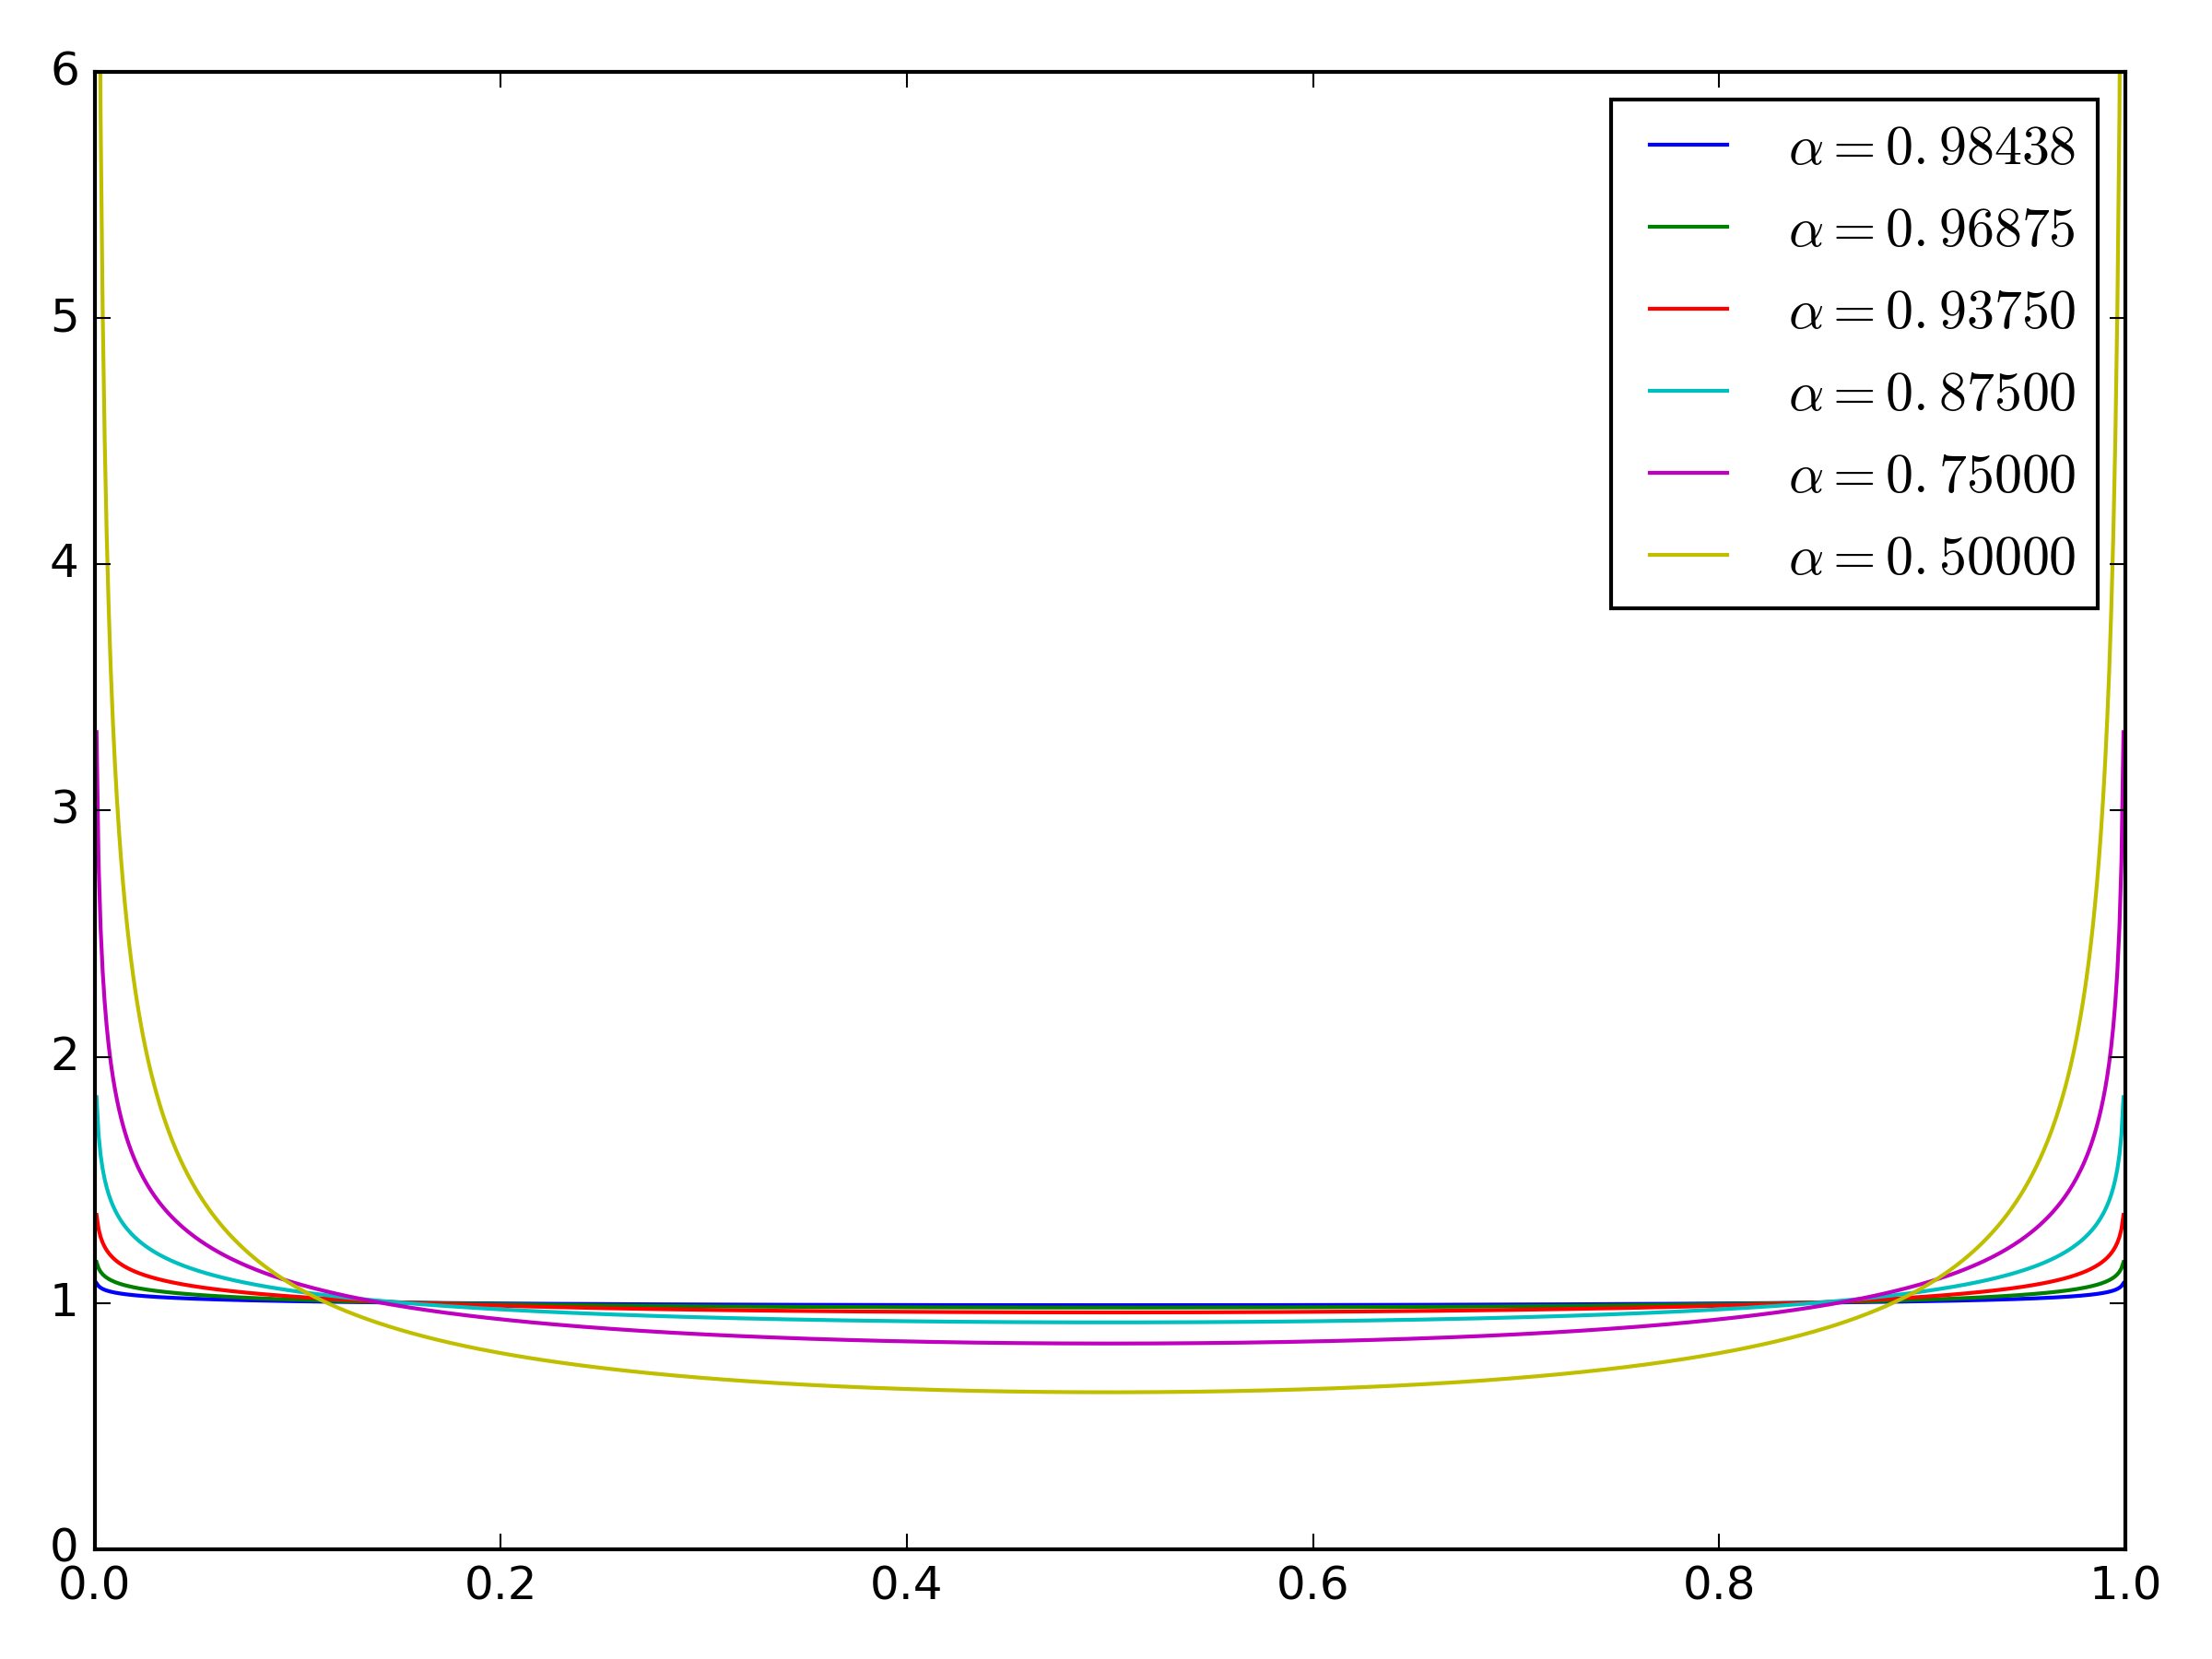
\includegraphics[width=0.65\columnwidth]{figures/beta.png}
	\caption{
		PDFs of Dirichlet distributions with 2D symmetric parameters $\alpha$. These can be used as a prior over the 2D PMFs. Note that this means there is $K-1 = 1$ degree of freedom, i.e. this is a prior for a Bernoulli random variable and this case is identical to a $\mathrm{Beta}(\alpha_0, \alpha_1)$ distribution. It is helpful imagine each of these curves as giving a distribution of probabilities for coins from an unfair coin factory, where the average over all coins looks fair, but (for large $\alpha \approx 0$) most individual coins are very unfair.
	}
	\label{fig:beta-pdf}

\end{figure}

It has mean $\boldsymbol{\alpha}_i / \sum_i \boldsymbol{\alpha}_i$ and when $\sum_i \boldsymbol{\alpha}_i < 1$ is said to be `sparse', meaning the pdf has most of its mass on the corners of the simplex, and typical samples have few non-zero entries. In the case of LDA, a symmetric Dirichlet prior is chosen, where $\boldsymbol{\alpha}_i = \boldsymbol{\alpha}_j ~~\forall i, j$, and the concentration, $\alpha = \sum_i \boldsymbol{\alpha}_i$, is considered as a hyperparameter. Fig.~\ref{fig:beta-pdf} illustrates the effect of varying $\alpha$. Choosing a symmetric, sparse Dirichlet prior for the topic-word distribution encodes the assumption that few words are strongly associated with a topic, some words are weakly associated with a topic, and most words are not at all associated with a topic without requiring any external information about which individual words are associated with which topics.

The posterior for $\theta$ given observations $z_i \sim Cat(\theta),~i = 1, \ldots n$ can be easily derived using Bayes' rule to be $P(\theta | \boldsymbol{N}) = Dir(\alpha + \boldsymbol{N})$, where $\boldsymbol{N}$ is the vector of counts for each of the $K$ possible values of $z$, and consequently the predictive distribution for $z_{n+1}$ is given by \citep{BishopCh2}:
\begin{equation}
\begin{split}
P(z_{n+1}=k | \alpha, \boldsymbol{z}) =& \int P(z_{n+1}=k | \theta) P(\theta | \alpha, \boldsymbol{z}) d\theta\\
=& \int \theta_k Dir(\alpha + \boldsymbol{N}) d\theta\\
=& \frac{N_k + \alpha}{\sum_{j=1}^K N_j + \alpha}
\end{split}
\end{equation}

Although exact inference of the full LDA posterior $P(\boldsymbol{z} | \boldsymbol{w})$ is intractable, the posterior for a single topic assignment $z_i$ can be estimated with a \todo{Double check we are collapsing variables} collapsed Gibbs sampler based on a the product of the predictive distributions due to $\theta$ and $\phi$ \citep{griffiths2004}. Given a set of observed words $\textbf{w}$, and topic assignments for all words except the current word, $w_i$, $\boldsymbol{z_{-i}}$ with counts $N^v_k$ being the number of times word $v$ was assigned topic $k$ and $N^k_d$ the number of times topic assignment $k$ has been used in document $d$
\begin{equation} \label{eqn:posterior}
P(z_i = k | \boldsymbol{z_{-i}}, \boldsymbol{w}) \propto \frac{N^k_d + \alpha}{\sum_{j=1}^K N^j_d + \alpha} \times
   \frac{N^{w_i}_k + \beta}{\sum_{v=1}^V N^v_k + \beta}
\end{equation}

Various other methods for approximate posterior inference for LDA have been explored, particularly variational methods and more recently stochastic gradient approximations to variational methods (For a comprehensive review, see \citep{geigle2016}). Despite the efficiency of these methods, they lack the appealing anytime, online aspect of a sampling based approach, and are much less flexible to modification of the model. For these reasons in this work we rely only on the Gibbs sampling based approach.

\section{Realtime Online Spatio-Temporal Topic Models}
\begin{figure}
\begin{center}

\subfloat[]{
\hspace{1.2cm}
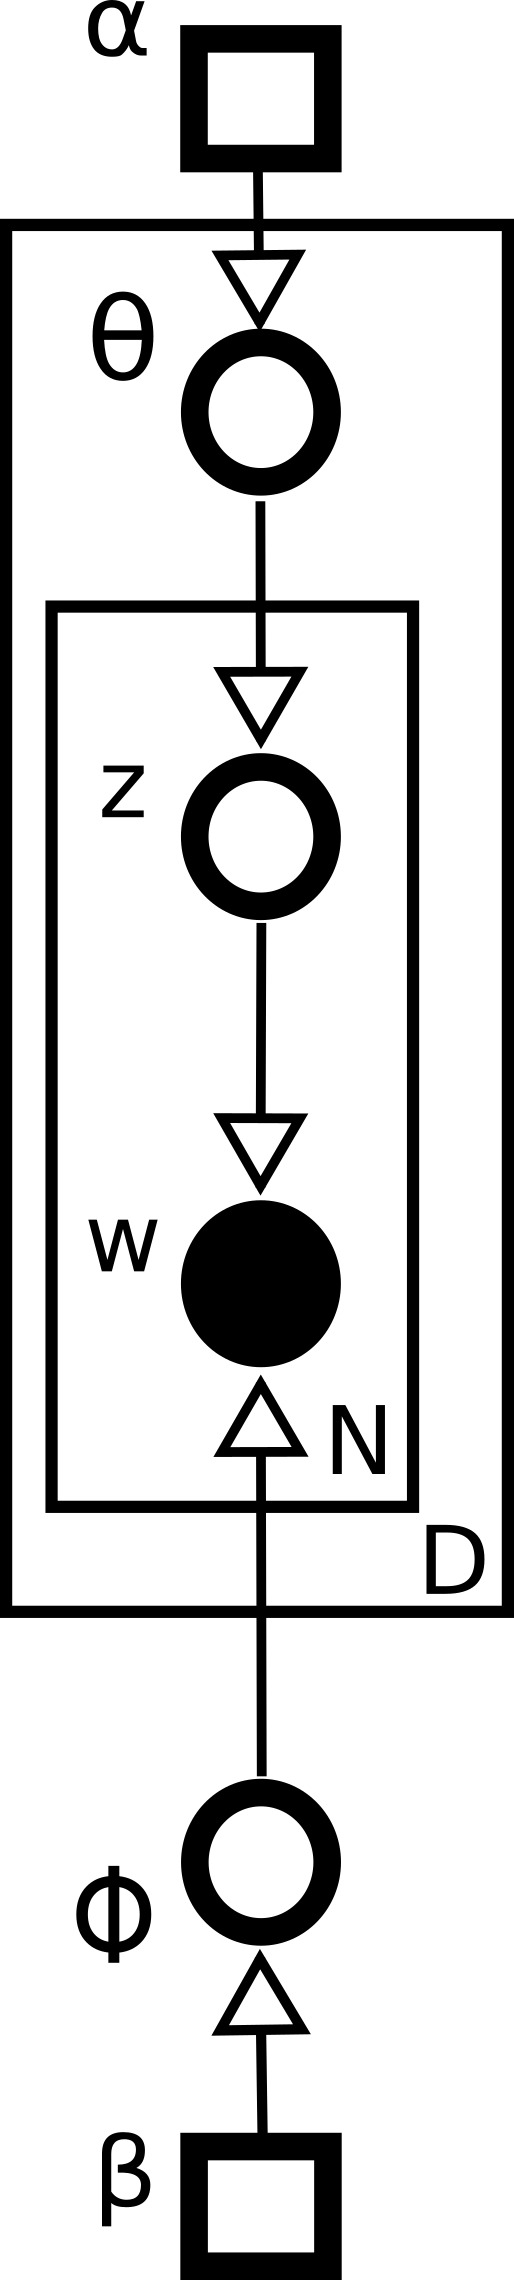
\includegraphics[width=0.13\columnwidth]{figures/lda_pgm.png}
\label{fig:lda-pgm}
} \hfill
\subfloat[]{
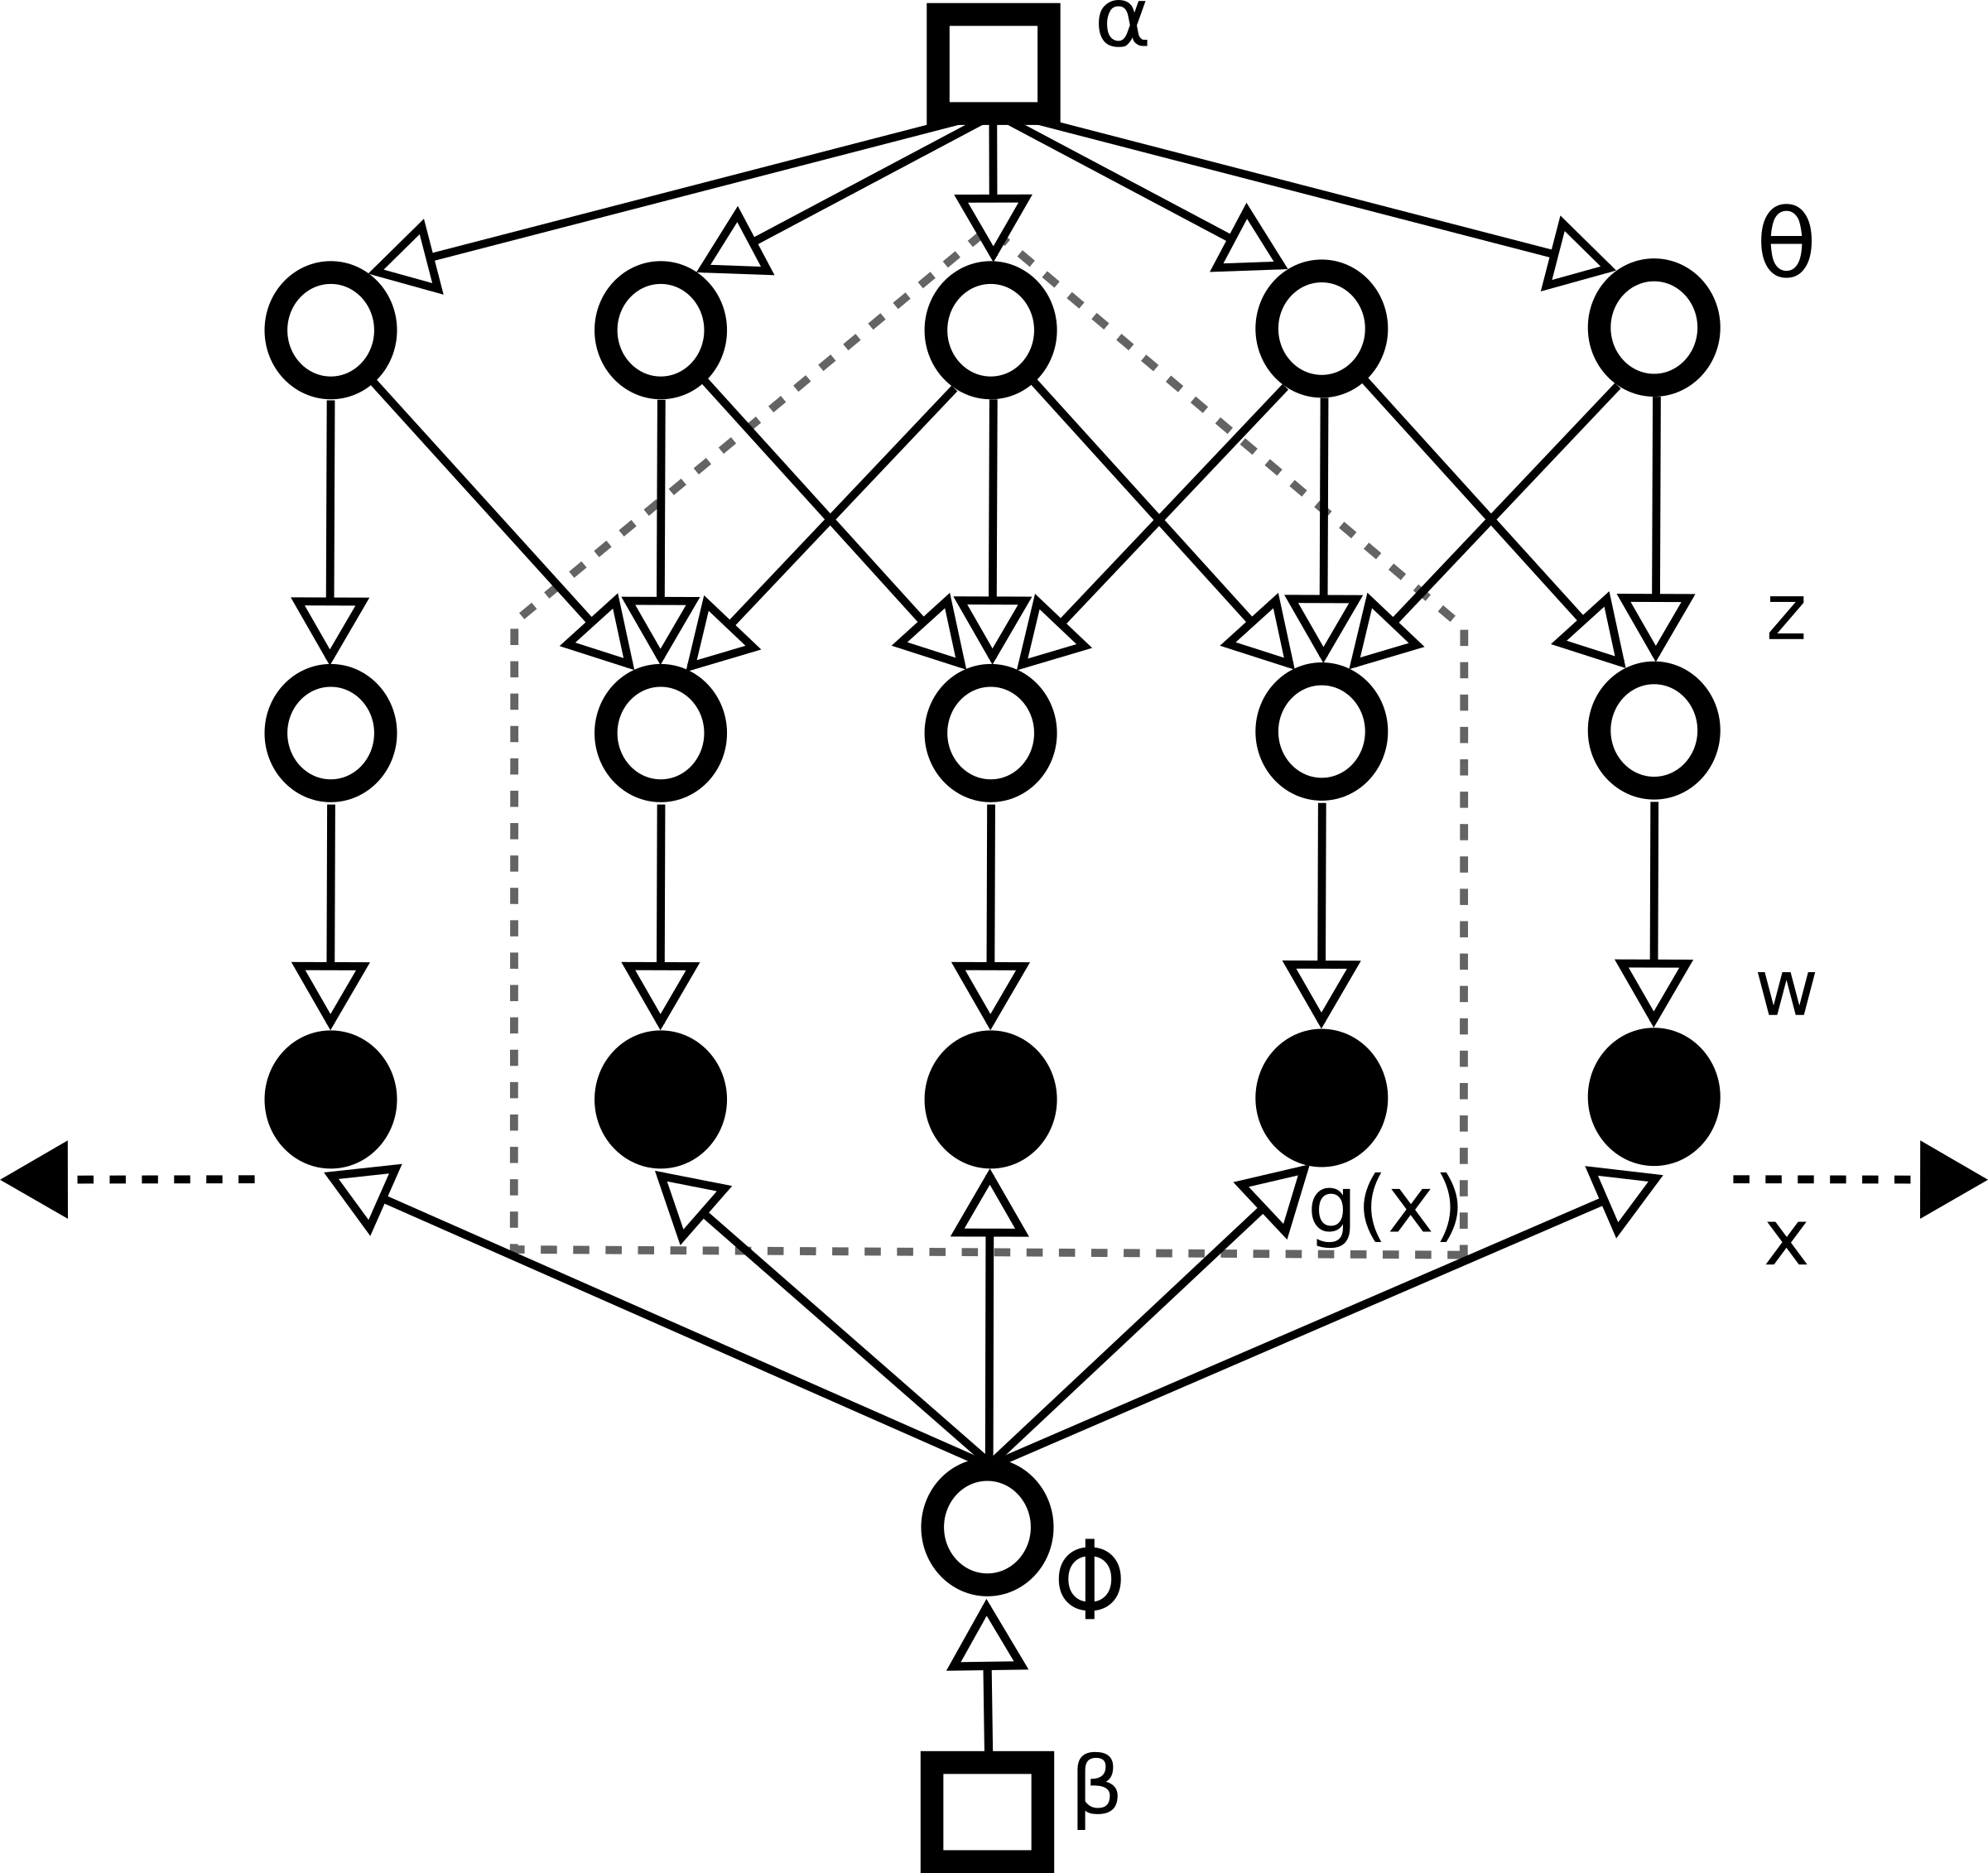
\includegraphics[width=0.6\columnwidth]{figures/rost_pgm.png}
\label{fig:rost-pgm}
}
\end{center}

\caption{
	\emph{Graphical models for topic models:}
	\protect\subref{fig:lda-pgm} Graphical model for Latent Dirichlet Allocation. Words within a document are conditionally independent given their topic assignments $z$ and the topics $\phi$, which in turn are conditionally independent given the topic prior $\theta$ for the associated document.
	\protect\subref{fig:rost-pgm} The graphical model for spatio-temporal topic models relaxes these independence assumptions, as the topic prior is shared by all topic assignments within overlapping spatio-temporal neighborhoods (represented by the dashed pentagon).
}
\label{fig:pgms}
\end{figure}

%%%%%%%%%%%%%%%%%%%%%%%%%%%%%%%%%%%%%%%%%%%%
%%% How has this been used for non-text? %%%
%%%%%%%%%%%%%%%%%%%%%%%%%%%%%%%%%%%%%%%%%%%%
Although LDA has been developed and used primarily in the context of modelling collections of text documents, its fundamental assumptions are compatible with an extremely wide range of applications. Virtually any feature function may be quantized or otherwise tweaked to produce discrete-valued pseudo `words' and collected into `documents'. Sparse, probabilistic `topics' are an attractive, interpretable form of dimensionality reduction for wide variety of domains. Non-textual descendents of LDA have most extensively been used in computer vision applications such as learning natural scene categories \citep{FeiFei2005}, taxonomies of images \citep{bart2011}, human action categories from video \citep{Niebles2008}, and image-caption pairing \citep{Blei2003Captions}. Further works illustrate how LDA can be used in bioinformatics, such as for learning genealogies (taxonomies of species) based on their collections of gene sequences \citep{Pritchard2000}. 

This body of literature hints that the LDA family of models is very general, and could be considered for a much broader set of applications where unsupervised representation learning is desired. One of the aims of this thesis is to demonstrate the breadth of this set. To clearly enumerate assumptions which must be met by an LDA application: (1) The data must be comprised of collections of discrete observations, (2) the observations within a collection must be conditionally independent given a set of topics and a prior over these topics, (3) the observations in separate collections must be conditionally independent given the topics and a symmetric Dirichlet prior, and (4) the topics must be conditionally independent given another symmetric Dirichlet prior.

%%%%%%%%%%%%%%%%%%%%%%%%%%%%%%
%%% What does ROST add? %%%
%%%%%%%%%%%%%%%%%%%%%%%%%%%%%%
Nevertheless, real-world data rarely meet these criteria exactly. In particular, observations associated with a particular place or time cannot usually be considered independent from nearby observations (Assumption 3). While we could accommodate this by simply increasing the size of our collections of observations, this choice would come at the cost of decreasing the spatio-temporal resolution of the learned document-topic priors. What we would like is to enforce smoothness rather than equality between nearby topic priors.

The Realtime Online Spatio-temporal Topic model ROST, implements exactly such a variant of Latent Dirichlet Allocation \citep{Girdhar2014}. With ROST, fully discrete \emph{documents} are replaced by \emph{neighborhoods}, each comprised of a topic prior and a collection of observations. We denote the neighborhood of a spatial, temporal or spatio-temporal location $x$ by $g(x)$. Crucially, neighborhoods may be overlapping, and consequently the priors for nearby neighborhoods are not independent -- instead they must describe an intersecting set of observations (see Fig.~\ref{fig:pgms}).

Formally, ROST includes the same 3 hyperparameters as LDA, namely $\alpha$, the Dirichlet prior concentration on each $\phi_z$, $\beta$, the Dirichlet prior concentration on $\theta_{g(x)}$ (with the neighborhood at $x$ replacing the document index $d$), $K$, the number of topics, as well as an additional hyperparameter, $g$, the spatio-temporal extent of a neighborhood. Increasing $g$ yields larger neighborhoods, where individual topic priors must account for more varied observations, are more overlapping with their neighbors, and therefore learning gives smoother document-topic distributions. Conversely, as $g$ decreases to 0, ROST becomes identical to LDA and the local topic priors have no tendency towards spatio-temporal smoothness. To implement posterior inference with the collapsed Gibbs sampler, the only change required to Eqn.~\ref{eqn:posterior} is to replace the document $d$ with the neighborhood $g(x)$ if word $w_i$ was observed at location $x$. \todo[inline]{Mention the kernel and $g_\sigma$?}

The authors have shown that the spatio-temporal smoothness assumption leads to more semantically relevant topics, in real-time computer vision problems as well as other domains \citep{Girdhar2012, Girdhar2014a, Girdhar2016}. The combination of smoothness and sparcity assumptions consistently leads the map of $\theta_x$ to contain regions with high probability of a single topic, with somewhat less-sparse boundaries between them. Because these assumptions are implemented as priors, precise knowledge of `how smooth' and `how sparse' is not required, in contrast to a harder or non-Bayesian approach. As a result, ROST produces remarkably natural, interpretable topic maps for a wide variety of datasets without an onerous hyperparameter tuning procedure.

\section{Topic Models in Practice} \label{sec:topic-models-inpractice}
Although topic models are a relatively robust modelling technique, recovering semantically meaningful topics still requires careful problem setup. This part of the process is often downplayed in the literature as less-than-generalizeable, nevertheless it is important to obtaining the desired data representation. The applications outlined in this thesis at least partially aim at exploring some of these issues, and how they can be systematized for varied applications and application domains.

%%%%%%%%%%%%%%%%%%%%%%%%%%%%%%%%
%%% Massaging the features   %%%
%%%%%%%%%%%%%%%%%%%%%%%%%%%%%%%%
The first issue encountered by an aspiring topic-modeller is how to obtain features which meet the assumptions of the model. Even in the text-modelling literature, where discrete-valued observations (words) and collections (documents) are readily available, significant pre-processing is common, including removing stop words and rare words, as well as stemming. These steps ensure a bag-of-words model is appropriate, ensuring that all the data is relevant to a semantic interpretation in addition to minimizing the importance of structure not captured by a histogram of words. These measures also have significant beneficial side-effects: stop words often comprise a significant portion of the dataset, so removing them significantly increases the variability between document-word distributions while greatly decreasing the total number of topic assignments to learn. In addition, stemming can greatly reduce the vocabulary, reducing the dimensionality of each word-topic distribution. In the context of natural language processing, these measures are acceptable -- the set of stop words in English is relatively small and can be easily listed, and reasonably performant stemming models are available.

Nevertheless, often the most difficult step in setting up a topic model is formulating a feature function with similar properties. In offline contexts, for a given feature function, filtering the most common and least common words is often a reasonable heuristic approximating removing stop words to enhance the variability between documents. In contrast, approximating stemming requires domain knowledge. Despite the challenge this entails, as we will describe in Sec.~\ref{sec:substrate}, it also presents an opportunity to insert a weak form of supervision beyond using purely pre-defined feature functions. By hand-coding or learning a relationship between raw features and data relevant to a semantic interpretation, the algorithm designer can refine the way in which the topic model will describe the data without resorting to the manual classifications that would be required for fully supervised techniques.

%%%%%%%%%%%%%%%%%%%%%%%%%%%%%%%%
%%% Choosing hyperparameters %%%
%%%%%%%%%%%%%%%%%%%%%%%%%%%%%%%%

Fortunately, although topic models are often used in situations where labelled classification data is impractical to collect, weak supervisory signals through cross-validation related to later, simpler, supervised learning problemsis are often enough to choose a model that captures the relevant insights. In the context of text-documents, this approach has been explored by Wallach et al. through a method to measure the semantic coherence of topics \citep{Wallach2009}. We take similar inspiration for non-text applications. Although this approach is expensive, requiring en exhaustive search of hyperparameter space, compared to DNN models, cross-validation is relatively cheap. This is firstly due to the hyperparameter space being much smaller, just 4 real-valued hyperparameters as opposed to the combinatorial space of DNN architectures. And is secondly due to the fact that topic model learning is much faster than fitting the most popular DNN architectures, on the order of just an hour on a consumer laptop for 1 million - 10 million word datasets.

The success of cross-validation through downstream tasks depends heavily on how we choose to interpret the topic model. Throughout the rest of this thesis each application will explore different ways of embedding the maximum-likelihood topic assignments, topic-word distributions, and document-topic distributions in tasks where providing ground truth is relatively easy. Many of these are focused on representations which are simultaneously simple to interpret yet still accurately capture the data. \todo{awkward last sentence}
%!TEX root = thesis.tex

\chapter{Soft, Unsupervised Classification with Spatio-Temporal Topic Models} \label{ch:topic-models-examples}
Our first two example applications explore the most direct connection to the existing topic modelling literature, performing unsupervised classification by defining a feature function, fitting a topic model, and grouping observations by their neighborhood's topic distribution. In Sec.~\ref{sec:substrate} we detail our work on deep-sea substrate classification from a challenging video dataset \citep{Kalmbach2016}. This application highlights the impressive closeness between the representation learned by our completely unsupervised technique and labels produced by a human expert which can be achieved by carefully designing a feature-function. Then in Sec.~\ref{sec:audio} we review our work on recognizing locations based on topic models of ambient audio \citep{Kalmbach2013}. This application highlights the suitability of spatio-temporal topic models for problems outside of computer vision, as well as the importance of spatio-temporal smoothness to representations learned in the absence of training targets.

\section{Substrate Classification from Repurposed Dive Videos} \label{sec:substrate}

\todo[inline]{Reduce the intro to this section?}\todo[inline]{I don't understand what you mean by "reduce", but this all ready pretty well to me as-is.}]
% \subsubsection{The need for soft substrate classifications from poor data}
% Paragraph: Why substrate classification matters
Substrate classification, the task of creating a spatial description of the nature of the seabed, is a fundamental factor in many aspects of ocean research.
Domain research in marine biology, physical oceanography and geology -- including classifying benthic \todo[inline]{say "(deep sea)" as well, this first time, for the CS person who doesn't recall what "benthic" means.} habitat, modelling deep-sea circulation and analyzing tectonic motion depends on accurate classification of substrate.

% Paragraph: Can't get enough hand labels
In the context of the deep sea, basic questions remain unanswered about what terrain can be found, particularly in geologically diverse mid-ocean ridge environments. High exploration cost and difficulty of sampling drive the need for remote sensing options for data acquisition, including visual and acoustic surveys, which in turn generate large volumes of data requiring analysis.
Manual analysis of substrate type is time consuming and requires geological expertise. Subjective factors, such as the choice of salient environmental features, make manual analysis for multidisciplinary use subject to observer bias.

% Paragraph: hard labels aren't really appropriate
Further, single-label classifications of substrate regions do not always adequately describe the complexity of types encoutered. In contrast, simple continuous valued substrate descriptors are sometimes used, such as the Udden-Wentworth Scale which proposes to describe the substrate by $-log_2(d)$ where d is average grain diameter in mm \citep{Krumbein1937}. Nevertheless, such descriptors are often impractical to evaluate with remote sensing, fail to capture the shape of the terrain, and do not account for the fact that terrain types, and therefore grain diameters, are rarely uniform within even a small region. Adding further dimensions to a substrate descriptor could account for some of these issues, at the cost of losing interpretability, and complicating the work of further domain research relying on this data. In this work we explore using soft classifications to add generality to the single-label paradigm, and seek to maintain interpretability by imposing a prior towards sparse label distributions. This approach can be seen as trying to maintain the best parts of both single label and higher dimensional substrate descriptors.

\begin{figure}
    \centering
    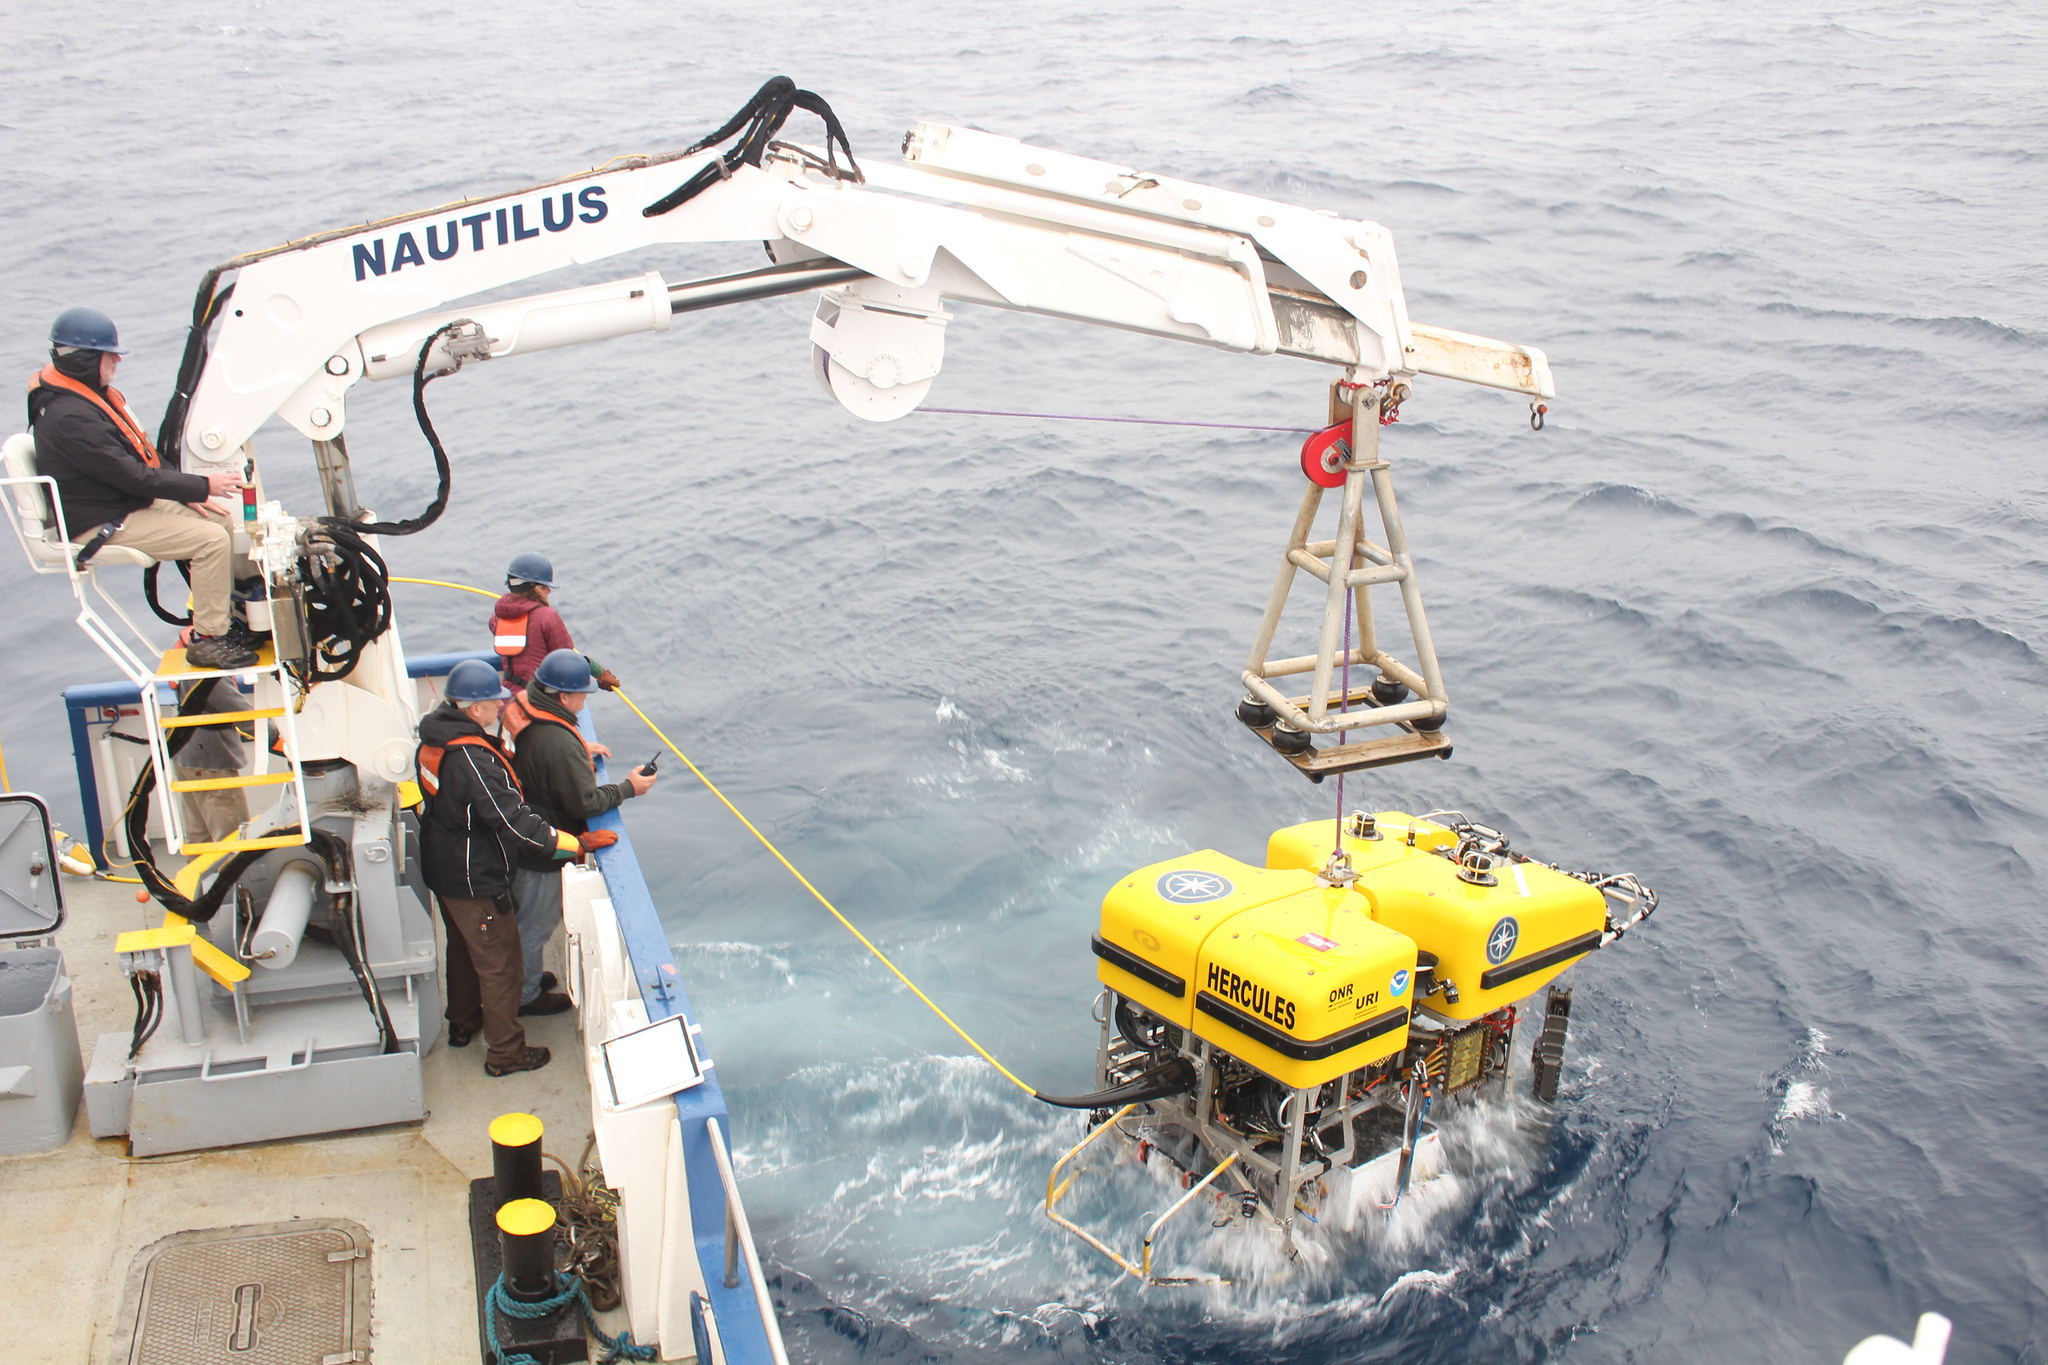
\includegraphics[width=0.65\textwidth]{figures/wacv/hercules}
    \caption{ROV Hercules returning to surface after a deep-sea cable route survey near Endeavour Ridge.}
    \label{fig:substrate-hercules}
\end{figure}
% 2-3 Paragraph: Can't just go get fresh data. Have to repurpose cable route surveys. Snow, lighting, and perspective.
Organizations such as Ocean Networks Canada (ONC), who operate cabled remote sub-sea observatories, regularly conduct manual visual cable route surveys in the deep-sea using Remotely Operated underwater Vehicles (ROVs). Collecting purpose-built deep-sea substrate measurements at high-spatial resolution is prohibitively expensive. In their absence, the historic video logs of these surveys contain extensive close-up video of the substrate, presenting the opportunity to train a substrate classification model.

Unfortunately, deep-sea ROV video contains significant artifacts due to a variety of factors. For instance hard, directional lighting is typical because sunlight does not reach the depths which interest us. Further, regions with the most interesting substrate such as hydro-geothermal regions, canyons, and seamounts all also feature challenging terrain for the ROV pilot. This leads to a wide variety of perspectives on the substrate. Finally, sediment and marine snow cloud the water column in the deep-sea, reducing contrast when the substrate is not very close to the camera, and filling images with particulate noise which confuses unmodified terrestrial computer vision techniques. Developing techniques to `see through' these artifacts to the substrate is necessary component of any system aiming to perform substrate classification using this data.

% Paragraph: ROST prior on classes is a reasonable assumption. So we just need to come up with a feature function that fits.
The spatio-temporal topic model's prior on neighborhood distributions is a good fit for this problem. It explicitly aims to capture the distribution of labels at each spatial location, rather than applying a single label like many techniques. Further, the sparse Dirichlet prior allows the modeller to ensure that the output distributions are more interpretable than a uniform or Gaussian prior when the meaning of the feature function is not well defined or understood with respect to the categories of interest. Finally, the smoothness component of the prior implemented by overlapping neighborhoods ensures that the topics reflect our intuition that labels at adjacent locations should be similar to one-another. By encouraging our model to capture our intuitions about the labels, we make the most of the large quantities of available unlabelled data so that with a highly restricted amount of labelled data we can learn to predict expert annotations.

\subsection{Using domain knowledge to define a feature function}

% 3 Paragraph: Feature extraction
As discussed in Ch.~\ref{sec:topic-models-inpractice}, one of the chief challenges of applying spatio-temporal topic models to a new domain is defining a feature function. In this work, we chose between standard, off the shelf, features combined with careful pre-processing steps to ensure that they encode the relevant information for substrate classification. Specifically we considered two feature functions: SIFT codebook and historgram of Improved Local Binary Patterns (ILBPs).

Based on the literature of topic models in computer vision, the most obvious choice of feature function is a codebook of Scale-Invariant Feature transform (SIFT) descriptors. SIFT is an extremely popular keypoint-based image feature, introduced by Lowe et. al as a scale and rotation invariant descriptor and detector for distinctive (i.e. easy to re-identify) points within an image \citep{Lowe2004}. SIFT has been remarkably successful in object recognition, image stitching, visual mapping, and many other computer vision tasks. We take SIFT as a reasonable surrogate for a variety of similar keypoint descriptors such as SURF and ORB. While SIFT features are 128-dimensional vectors, our topic models require discrete-valued features (words). Before running our algorithm, we produce a codebook of SIFT features. That is, using ROV logs from other dives, we compute the keypoints and descriptors for each frame. Then, choosing a vocabulary size (i.e. $V = 3000$), we compute the $V$ k-means centroids. At training time for our topic model we then extract keypoints for each new frame and compute the descriptors for each, replacing the descriptor with the index of the nearest neighbor centroid.

In contrast, Local Binary Patterns represent textures by encoding the local brightness variations in 9-pixel squares as 8-bit codes representing the relationship between each edge pixel and the center. Typically, these codes are computed for every pixel in an image, and grouped together into 256-bin histograms for non-overlapping windows. These histograms are then used as a descriptor for the textures in their windows. ILBP, originally introduced under the name MultiBlock LBP in \citep{Liao2007}, extends LBP, firstly by accommodating scaled pixel areas, and secondly by adding information about the center pixel. In ILBP, each pixel, including the center pixel, is compared to the mean value over an $N \times N$ pixel region. Liao et al. have shown that this improves the robustness of LBP as well as the ability to encode larger image structures. We use the multi-channel, multi-scale, windowed ILBP implementation described in \citep{Paris2012}. In contrast to descriptors such like SIFT, ILBPs are usually collected directly as histograms, and therefore no codebook is necessary. We concatenate the histograms for each window, scale, and color channel of an image, and treat each bin of the resulting histogram as a discrete feature when running our model.

% 2 Paragraph: Frame-rejection and resampling
In order to ensure that our model learns to distinguish substrate types, and not some other aspect of the dataset, it is important to carefully choose what data we will model.
A typical cable route survey creates 6-12 hours of continuous dive video, of which at least a few hours are usually irrelevant. For instance, surveys often contain extensive video of the ROV descending or ascending, sections with minutes to hours of video where the ROV is parked on the sea-floor, and yet more sections where the substrate is not in view due to challenging navitational conditions and sediments disturbed by the ROV itself.
Further, it is atypical for surveys to be conducted at constant speed, as the video is designed for live, manual analysis. To counter these effects, we first train a substrate detector, and then select a set of training images that are uniformly distributed in space.

We implement a substrate detector with a support vecor machine (SVM) on the spatial envelopes of relevant and irrelevant frames.
By spatial envelope, we refer to the holistic representation of the shape of a scene implemented as the GIST
descriptor described in \citep{oliva2001GIST}. GIST descriptors have been shown to encode high-level perceptual dimensions of the
spatial envelope such as ‘naturalness’, ‘openness’, ‘roughness’ etc. This descriptor is computed using a method based on Gabor filter responses in multiple orientations and scales, and in a grid of image windows across the image. GIST descriptors are appropriate as the local appearance of images with substrate varies dramatically, and the spatial envelope is more important that any local features.

We manually labelled 2000 randomly selected frames as either relevant or irrelevant (i.e. with or without substrate) for our subsequent classification problem. We trained an SVM using 1000 frames randomly selected from these 2000 labelled examples, and evaluated its performance on the other 1000. Table~\ref{tab:GIST-svm-performance} shows the precision and recall computed over all frames in the test set.

\begin{table}[t]
    \begin{center}
      \begin{tabular}{|c|cc|}
      \hline
         & Substrate & No Substrate \\
        \hline\hline
        Train Set (True)         & 564  & 436 \\
        Test Set (True)          & 589  & 411 \\
        Full Dataset (Estimated) & 6859 & 3141\\
        \hline
      \end{tabular}
      \caption{Numbers of relevant and irrelevant frames in our example video.}
      \label{tab:detection-statistics}
    \end{center}

    \begin{center}
      \begin{tabular}{|c|ccc|}
        \hline
         & Precision & Recall & F1-Score\\
        \hline\hline
        Train Set & 0.7942 & 0.9645 & 0.8711\\
        Test Set  & \textbf{0.8117} & \textbf{0.9440} & \textbf{0.8729}\\
        \hline
      \end{tabular}
      \caption{Performance of GIST SVM substrate detector.}
      \label{tab:GIST-svm-performance} 
    \end{center}
  \caption{GIST SVM performance}   
\end{table}

Dive logs contain navigation data collected by an ultra-short baseline (USBL) acoustic positioning device, in the form of Latitude, Longitude, and Depth measurements in addition to video. We converted Lat., Lon. into Eastings and Northings (meters East or North from start point), and time-synchronized the navigation and video logs. Next we ran our substrate detector on each frame from the video, discarding frames which did not contain substrate. Finally, we constructed a topic model training set by passing through the data in temporal order, and only keeping video frames which were more than a fixed radius away from all other points in the training set.

% 2 Paragraph: Image + feature filtering
In addition to ensuring that the training data comes only from potentially relevant locations, we must also ensure that the features encode the relevant aspects of the images.
Most images in the survey videos contain strong brightness variation at a low spatial frequency due to hard directional lighting and not the shape or texture of the substrate. Typical frames contain a well-lit foreground in the bottom middle and darker regions elsewhere. Due to marine snow and sediment, many images also contain particulate noise.
As perspective and other conditions change, these factors vary. To mitigate this,\todo[inline]{What is "this"}? we apply a 2D Gaussian bandpass filter with kernel
\todo{I suggest saying, to reduce the visual impact of the irrelevant, but ubiquitous, particular matter that is manifested as high-frequency image content, we use a bandpass filter"}
\begin{equation}
K = (1-e^{-(x^2+y^2)/2f_{low}^2}) \times e^{-(x^2+y^2)/2f_{high}^2}
\end{equation} 
where we set the frequency cutoff parameters $f_{low}$ and $f_{high}$ to be 4 and 100 cycles/image respectively based on the approximate minimum and maximum size of relevant substrate features. While particulate noise was a low spatial frequency detrimental factor, we found that the SIFT keypoints lost by smoothing over image details were more detrimental. To compensate, before extracting SIFT features we applied the highpass Guassian filter only. Finally, even with these preprocessing steps, not all features contain enough variation to help distinguish frames, and therefore only contribute noise to the modelling process. The concatenation of all the LBP histograms for an image results in a 10,752 dimensional histogram. We found that keeping only the $V = 3000$ bins with highest variance greatly reduced inference time for our topic model while slightly improving classification performance.

\begin{figure}
\begin{center}

\subfloat[]{
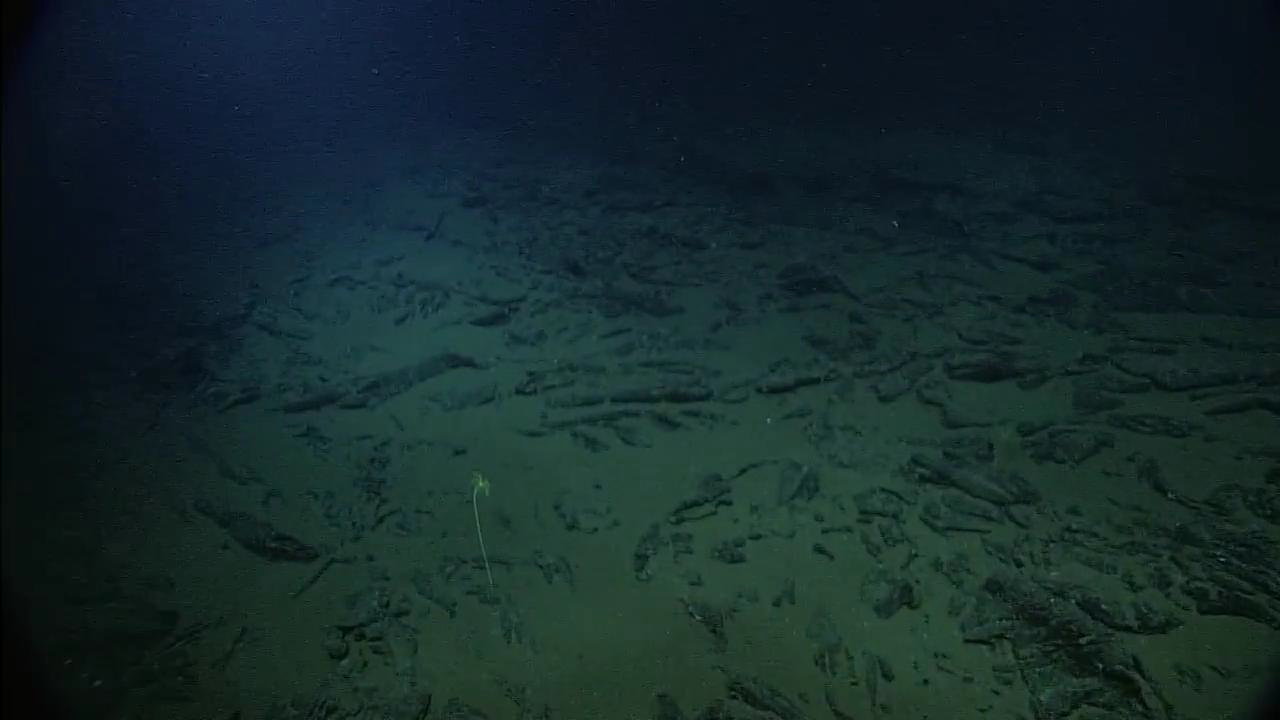
\includegraphics[width=0.48\columnwidth]{figures/wacv/r1218-beforefilter}
\label{fig:rov-eg-before}
}%
\subfloat[]{
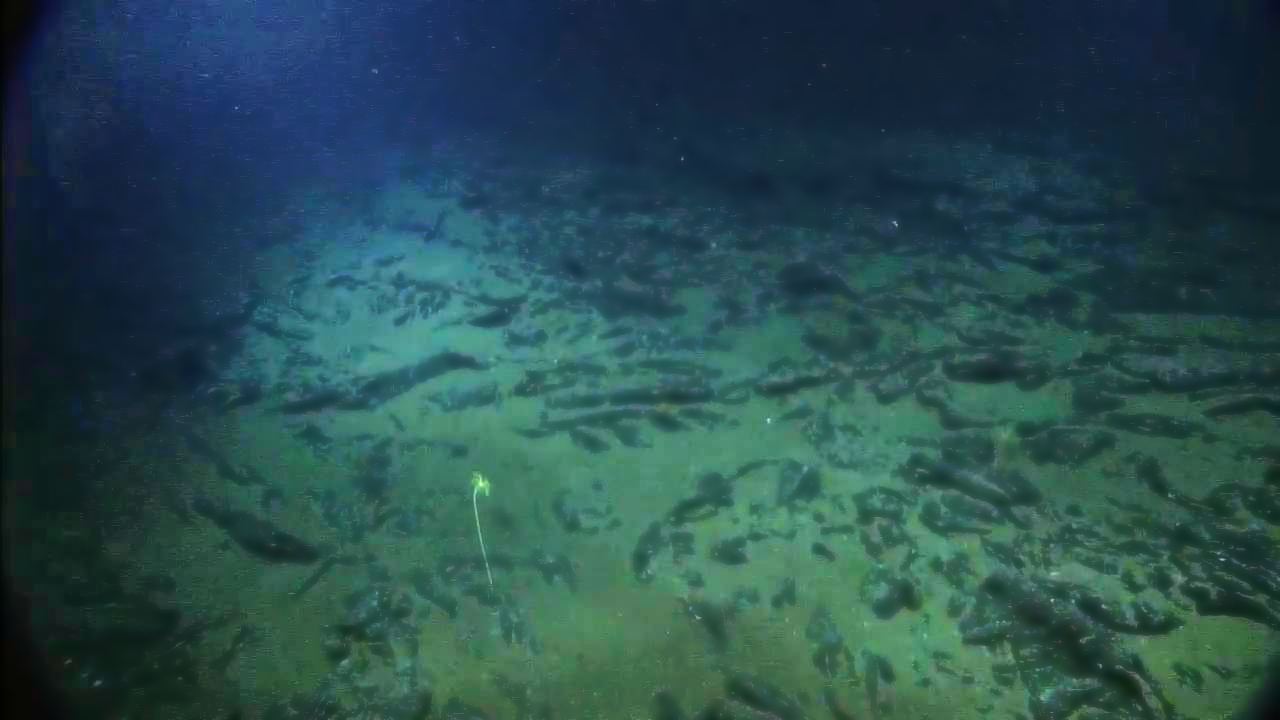
\includegraphics[width=0.48\columnwidth]{figures/wacv/r1218-afterfilter}
\label{fig:rov-eg-after}
}
\end{center}

\caption{
    \emph{Challenging ROV video data:}
	\protect\subref{fig:rov-eg-before} An example image collected by the ROV, before bandpass filtering and 
	\protect\subref{fig:rov-eg-after} after. 
}
\label{fig:rov-eg}
\end{figure}

\subsection{Evaluation}

% 2 Paragraph: Dataset description
We validate our method using data recorded at the Endeavour Segment of the Juan de Fuca Ridge, a midocean
ridge environment 300 km West of Vancouver Island, British Columbia, at approximately 2.2 km depth \citep{endeavourMPAPlan}. Specifically, our data is from the East Flank of Endeavour, a gently sloping area featuring a variety of substrate types. Mission objectives on this dive were to perform a visual survey for suitability of a scientific instrument installation -- much of the video shows substrate, but distance, angle, and speed are inconsistent throughout the recording.

The data consist of 30 fps HD video and 10 Hz USBL acoustic positioning. The ROV moved at an average rate of 0.5 knots (approx. 0.26 m/s), through two partially overlapping lawnmower patterns, one up and down a gentle slope, and one across the flat area at the base of the slope, with a total distance travelled of just over 5.6 km. We ran the substrate detector on every third frame (synchronized with the USBL data), and applied spatial subsampling with a minimum inter-frame distance of 1.5 m. This process resulted in a dataset of just over 3000 images.

Of these, we randomly selected 500 images, and with guidance from an expert in deep-sea geology, we defined seven categories that represent the types of substrate seen in the sample. These categories were ‘Sedimented’ (SED), ‘Interrupted Lava Flow’ (INT), Pillow Lava Flow’ (PIL), ‘Cliff or Wall’ (CLIFF), ‘Other Rock’ (O.RCK), ‘Turbid Water’ (TURB), and ‘Substrate out of Range’ (DARK). We labelled each image in this sample with proportions of these seven types, using a minimum increment of 0.25 for each category. Images exemplifying each category can be seen in Fig.~\ref{fig:substrate-best1gt}.

% 3 Paragraph: Pairing topics and classes
We generated the SIFT and LBP bag-of-words representations for each image in the full dataset, using the noise supression techniques described above. We used scale factor 2 for the ILBP region with a uniform 6x7 grid of non-overlapping windows. Initial experimentation showed that these values produced good results, and that additional scales did not cause significant improvement. We then fit the spatio-temporal topic model on each feature representation, choosing a neighborhood size of 15 m and 7 topics based on the estimated variation of the terrain and the number of true categories. We repeated this process for each pair of sparcity hyperparameters $\alpha, \beta \in \{0.01, 0.1, 0.2, 0.4, 0.8, 0.9, 0.99\}$. We chose the model with maximum log-probability on the held-out 500 image labelled set: $\alpha = 0.1, \beta = 0.1$ for SIFT and $\alpha = 0.1, \beta = 0.8$ for LBP. For these 500 datapoints, we infer topic assignments without updating the model. Although the most extreme values of $\alpha$ and $\beta$ tended to perform poorly, intermediate values had similar log-probabilities, and the exact hyperparameter choice did not seem to have a strong effect on the learned topics.

To evaluate the degree to which each ground-truth category was represented by some topic generated by our algorithm, we produced a one-to-one pairing between categories and topics. First, we calculated the Pearson $\rho$ correlation between each ground-truth category and each topic produced by our algorithm, using all 500 of the ground-truth frames. Then, we defined the cost of associating category $i$ with topic $j$ as $Cost(i, j) = 1 - \rho_{i,j}$, and used the well known Kuhn-Munkres (`Hungarian') Algorithm \citep{KuhnHungarian}, to find a minimal total cost assignment. In other words, we paired categories and topics so as to maximize the sum of correlations in the set of pairings. As the pairing is between topics and classes (a $7\times7$ matching problem), the cost of this process is negligeable.

We also computed 7 k-means centers for each image based on the distribution of each feature; SIFT, LBP, and top-3000-dimensions LBP. Then, we computed the cluster labels for test images, and applied the same optimal pairing algorithm for each. The results of these approaches offer insight into how well a method which does not take spatial smoothness into account might perform.

% 2 Paragraph: Describe tables. Impressive performance considering tiny amount of training data.
Fig.~\ref{fig:substrate-exout} shows the most representative frames for each topic. These images show the 7 frames that have the highest proportion of each topic throughout the dataset. Note that some topics were much more prevalent than others, so
an image may be among the best examples of a particular topic in the dataset without that topic being the top label for
the image. For instance, many of the strongest examples of interrupted lava flows contain more sediment than interrupted
lava flow. Comparison with the examples in Fig.~\ref{fig:substrate-best1gt} suggests that the topics assigned
to sediment, turbid water, and substrate out of range accurately recover their categories, and that the
other assignments are somewhat less accurate.

Tab.~\ref{tab:substrate-performance-7} reports the correlations between topics (or cluster labels) and ground-truth labels in the optimal pairing. Note that the topic model obtained the highest correlation of any method for every category, improving the strength of association by a mean of $3.58$ times over the best k-means approach (strength of association is defined as the absolute value of correlation). Strong positive correlations (i.e. near 1) indicate a linear relationship between variables, in this case indicating that the proportion of an image composed of a certain label can be predicted by a linear function of the weight of a single topic much more confidently than from its k-means cluster assignment. Also note that the LBP topic model outperformed the SIFT topic model for all classes except pillow lava, while at the same time the LBP k-means models also outperformed the SIFT k-means model for all classes except pillow lava. This suggests that the performance of a simplistic k-means model may be a reasonable simplistic surrogate for the full topic model when choosing which feature function to use for a topic model.

Note that for the LBP topic model, p-values were $ \lll 0.001 $, whereas for the other approaches, p-values varied, sometimes taking significantly higher values.
These p-values represent a strong rejection of the hypothesis that the topics were not correlated with the categories for our method, and a weaker one for the baseline strategies.

\begin{figure}
    \begin{minipage}{0.285\linewidth}
        \subfloat[][]{
            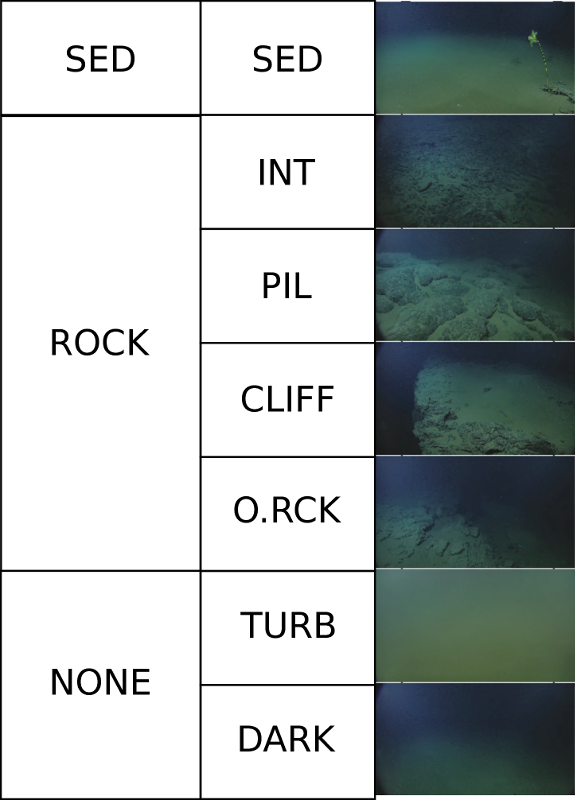
\includegraphics[width=0.979\textwidth]{figures/wacv/best1gt_table.png}
            \label{fig:substrate-best1gt}
        }
    \end{minipage}%
    \begin{minipage}{0.69\linewidth}
        \subfloat[][]{
            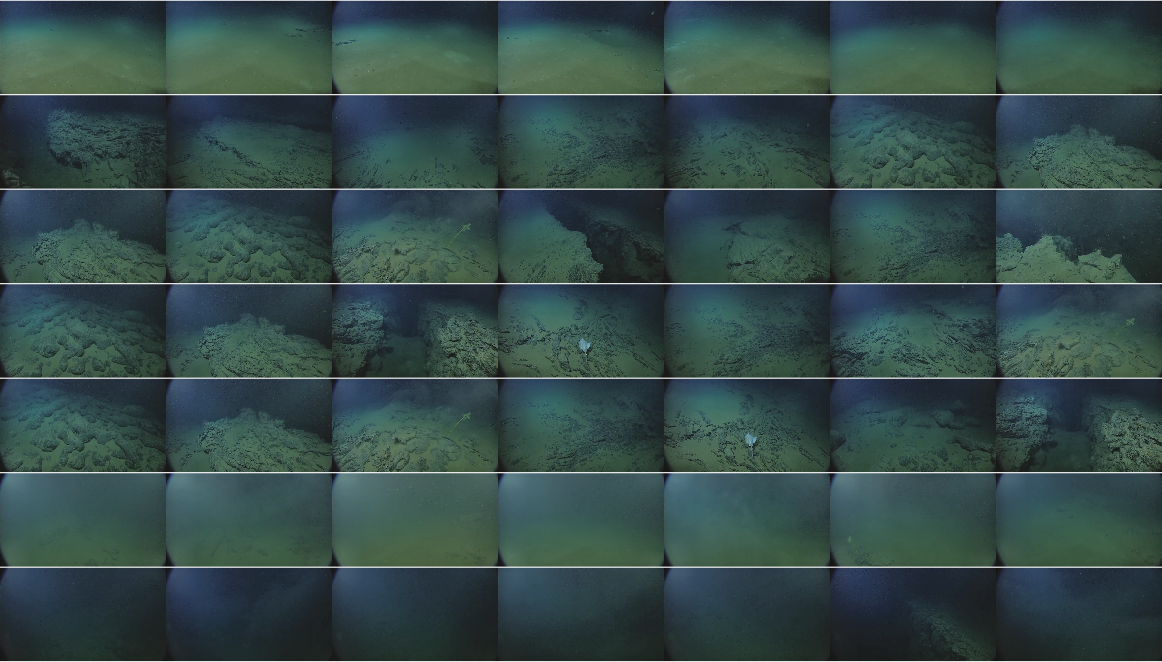
\includegraphics[width=0.98\textwidth]{figures/wacv/exout7.png}
            \label{fig:substrate-exout}
        }
    \end{minipage}
  \caption{
  	\emph{Example images of substrate types, and paired topics:}
    \protect\subref{fig:substrate-best1gt} Representative examples of the categories (top to bottom) `Sedimented', `Interrupted, 'Lava Flow'  `Pillow Lava Flow', `Cliff or Wall', `Other Rock', `Turbid Water', and `Substrate out of Range'.
	\protect\subref{fig:substrate-exout} Top 7 images paired with each category from
	\protect\subref{fig:substrate-best1gt}, based on the max-likelihood topic distribution, and the max-correlation pairing algorithm.
  }
  \label{fig:substrate-examples}
\end{figure}%

\begin{table}
    \centering
    \caption{\emph{Detailed substrate classification performance:}
    Pearson $\rho\left(498\right)$ for best-match topic with 7 ground truth categories (see \ref{fig:substrate-best1gt}). For ROST Filt. LBP p-value was $\ll 0.001$. Our method had the highest correlation for every category except PIL}
    \begin{tabular}{|c|ccccc|}
        \hline
              & K-M SIFT & K-M LBP & K-M Filt. LBP & ROST SIFT & \textbf{ROST Filt. LBP}\\
        \hline \hline
        SED   &  0.2898 &  0.3526 &  0.3661 & 0.5196 & \textbf{0.7489} \\
        INT   &  0.0718 &  0.0092 &  0.1116 & 0.3517 & \textbf{0.3899} \\
        PIL   &  0.4162 & -0.0029 &  0.0849 & \textbf{0.7024} & 0.3884 \\
        CLIFF &  0.1721 &  0.3474 &  0.2916 & 0.3601 & \textbf{0.4152} \\
        O.RCK & -0.0137 &  0.0508 & -0.0685 & 0.1901 & \textbf{0.2580} \\
        TURB  & -0.0271 &  0.6385 &  0.7509 & 0.1723 & \textbf{0.8153} \\
        DARK  &  0.3630 &  0.7509 &  0.3466 & 0.5454 & \textbf{0.5664} \\
        \hline
    \end{tabular}
    \label{tab:substrate-performance-7}

    \caption{\emph{High-level substrate classification performance:}
         Pearson $\rho\left(498\right)$ for best-match topic with 3 high-level categories. Our method had correlation coefficient above 0.7 for every category, with p-value $\ll 0.001$.}
    \begin{tabular}{|c|ccccc|}
        \hline
             & K-M SIFT & K-M LBP & K-M Filt. LBP & ROST SIFT & \textbf{ROST Filt. LBP}\\
        \hline \hline
        SED  &  0.4413 &  0.5059 &  0.5350 & 0.5196 & \textbf{0.7489} \\
        ROCK &  0.3492 &  0.3541 &  0.4930 & 0.6852 & \textbf{0.7156} \\
        NONE &  0.0459 &  0.4930 &  0.4601 & 0.3116 & \textbf{0.8015} \\
        \hline
    \end{tabular}
    \label{tab:substrate-performance-3}
    
\end{table}

In absolute terms, the values of the correlations reflect the intuition given by the best examples of each topic: The categories sediment, turbid water, and no substrate are each strongly correlated with their assigned topic, but the other categories are only weakly correlated with their assignment. Therefore, we additionally analyze our system's performance in classifying the high-level categories ‘Sediment’, ‘Rocky’, and ‘No Substrate’. These categories were constructed by combining the original categories, as seen in the leftmost column of Fig.~\ref{fig:substrate-examples}. We combined the groundtruth labels, topics, and labels for the three baseline methods by summing over the groups to be combined into each of the three categories. The performance of the resulting models is presented in Table~\ref{tab:substrate-performance-3}, showing that the LBP topics show strong predictive ability for the high-level class labels.

\begin{figure}
    \centering
    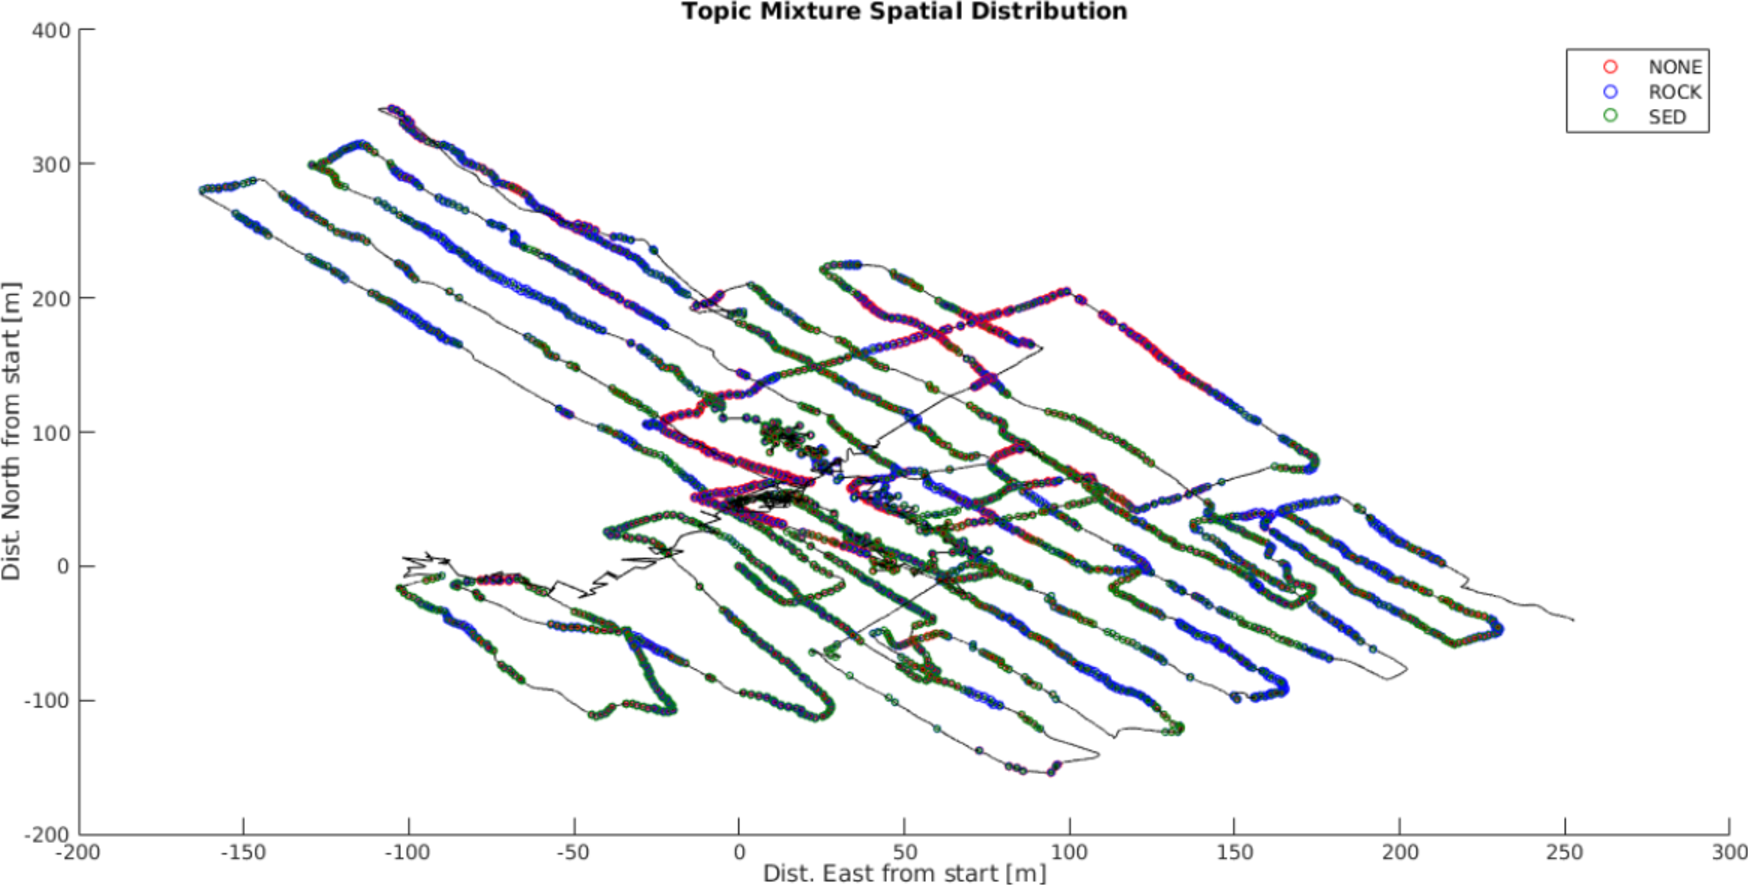
\includegraphics[width=0.9\textwidth]{figures/wacv/mixture-map2.pdf}
    \caption{\emph{Estimated substrate mixture map for Endeavour Ridge, BC:} ROV track with topic mixtures at each sample point. The line represents the path of the ROV, and each point is the location of a substrate sample image. At each point, there are circles for each of the three topics, with their sizes representing the mixture of the topics in that sample.}
    \label{fig:substrate-topic-map}
\end{figure}

Finally, in Fig.~\ref{fig:substrate-topic-map} we present the map of high-level substrate types produced by the LBP topic model. Maps of this type provide an interface between our method and biological or geological research which seeks to use information about substrate type. For instance, this map could be used in conjunction with a map of observations of a certain species to help answer questions about how habitat suitability is related to substrate type. Note that most points are described mainly by a single type, and that the substrate type assignments are spatially consistent. This outcome is crucial to an intuitive understanding of the map; it allows scientists to think naturally about regions of the substrate while still admitting that transitional areas which cannot be labelled as a single type exist. By choosing a spatial topic model to capture the visual data, we explicitly require our method to recover such an interpretable model. The automatic substrate classifications of our work are included in the GIS database for the Endeavour marine protected area, and are publicly available to researchers interested in the area \citep{Douglas2017} \footnote{An interactive version of this database is avilable online at \url{http://www.oceannetworks.ca/endeavour-hydrothermal-vents-marine-protected-area}}.

\section{Same-Place Recognition from Ambient Sound} \label{sec:audio}
%%% What happens when we try a very different feature function to text or bag-of-image-features? %%%
%%% How are semantic closeness, feature closeness, and topic closeness related? %%%
%%% 8 pg %%%

Our second example application of spatio-temporal topic models highlights the versatility of the model, operating on features from ambient audio. To the best of our knowledge, this is the first application of topic models to environmental audio that takes advantage of spatially coherent semantic regions. Our ability to consider temporal dependencies is crucial for this application as sound is fundamentally linked to temporal variation.

In this work we consider how to identify similar world regions by modelling the statistics of ambient sounds. We hypothesize that transitions in acoustic space correlate with transitions in other characteristic properties of the environment. Therefore, we aim to use the ambient sound to identify particular places and detect when we have returned to places we have already visited. In the context of robotics, we envision this system as one of many inputs to a filter-based probabilistic localization system. Common sensors such as range-finders and cameras often produce precise location hypotheses, but they are also susceptible to ambiguities which give rise to multi-modal beliefs. In contrast, an ambient-sound based localization system would give relatively imprecise hypotheses, only identifying the high-level region rather than an exact pose. However ambiguities in the soundscape of an environment are potentially very different from keypoint or corner ambiguities which confuse traditional sensing modalities. As a result, even such `weak' loop closures from sound could help improve the performance of localization systems.
\todo{Ambiguities... however ...}

Similar to the substrate classification example, in this work, an agent traverses the environment, makes observations along the way, and seeks to produce an intuitive description of these observations. As with substrate classification, an intuitive account is one that describes the world in terms of a few types, where neighboring locations should be assigned to the same type most of the time. Our spatio-temporal topic modelling framework aims to exploit this intuition to learn an appropriate representation without using any ground-truth labelling.

As we are interested in an input to a localization system, in this example the topic model features temporal smoothness rather than spatio-temporal, and observations are not accompanied by their position in the world. In addition, this system is designed to be fully unsupervised. That is, rather than matching topics with labels from a small training set, in this work we allow the topics to describe the data in whatever way represents it most accurately, and aim to extract information by comparing topic priors for different temporal neighborhoods to one-another directly.

\todo{Would be really nice to have a picture of the physical system (husky) and/or local region at ground level. Do you have either? Not critical, of course.} 

\subsection{Acoustic Features}
In the previous example we have seen the importance of carefully designing a feature function. For this example, we must take a short window of ambient audio and turn it into a discrete-valued feature. We extract such a feature using a k-means codebook of Mel Frequency Cepstral Coefficients (MFCC).

MFCCs are a compact representation of the timbre of an acoustic signal over a short time window. They have been commonly used to detect the source of a signal, especially in speaker and instrument recognition problems. Successive coefficients of a cepstrum represent the amount of the signal due to increasingly complex sinusoids. These are calculated using the inverse DFT of the log of squared DFT magnitude of a signal. MFCCs in particular use a re-weighting of the magnitude spectrum, so that lower frequencies are treated as more important than higher ones in order to achieve a more perceptually relevant cepstrum.

To be exact, MFCCs are computed using a filter bank with $L$ overlapping bands with triangular magnitude responses $\hat{h}_{l}[k]$ for $l=1, 2, ..., L$. The center frequency of band $l$ is given by $f_c(l) = 700 (e^{l/1127} - 1)$. The overlap percentage is constant and the centers are spaced further apart as frequency increases (see Fig.~\ref{fig:audio-melbank}), resulting in higher precision and weight on the lower frequency part of the signal. Given an input window $x$ the Mel-Frequency Cepstrum is given by
\begin{equation}
    cc(x) = \left| \mathcal{F}^{-1} \left( \log\left( \left|
    \sum_{l=0}^L
    \mathcal{F} \left(x\right) \hat{h}_l
    \right|^2 \right) \right) \right|^2
\end{equation}
The first $M$ coefficients can be computed efficiently using a DCT formulation where the filterbank is applied directly to the time-domain signal. In this domain, an interpretation where the $m$-th coefficient represents the part of the signal that can be described by the $m$-th cosine basis function arises.

\begin{figure}
    \centering
    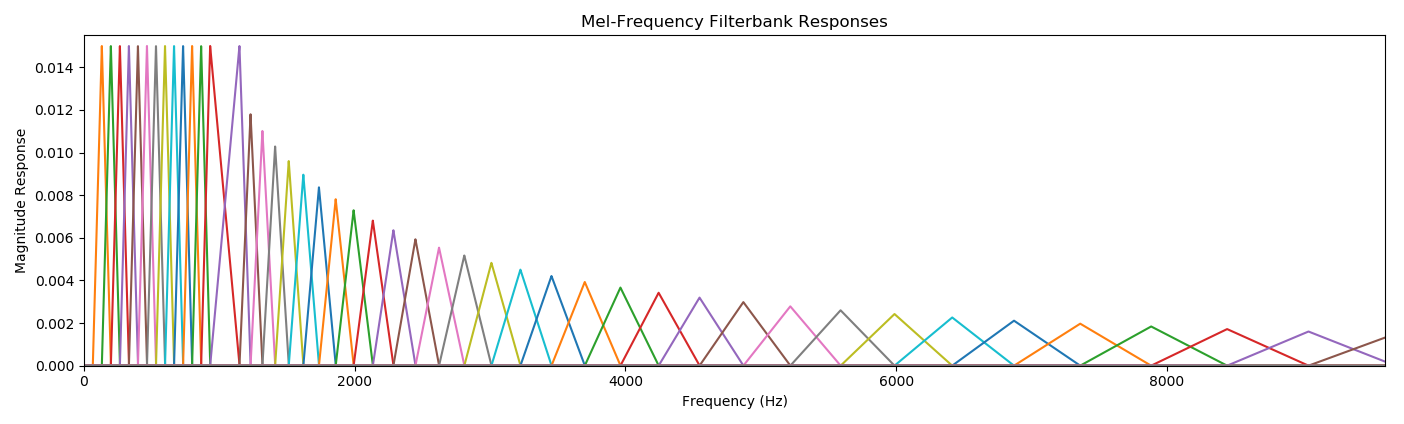
\includegraphics[width=\textwidth]{figures/audio/mel-responses.png}
    \caption{Mel- filterbank $h_l$ frequency responses for 48-bands and 50\% overlap. This filterbank implements perceptual reweighting of an audio signal.}
    \label{fig:audio-melbank}
\end{figure}

We consider the truncated cepstra, i.e. the first $M$ coefficients for short, overlapping windows of audio, as is typical for instrument and speaker identification problems which employ cepstral techniques. More detail on the construction of the filter bank and on choosing appropriate parameters for the window size and number of coefficients to calculate can be found in \citep{Sturm2010}.

\begin{figure}
    \centering
    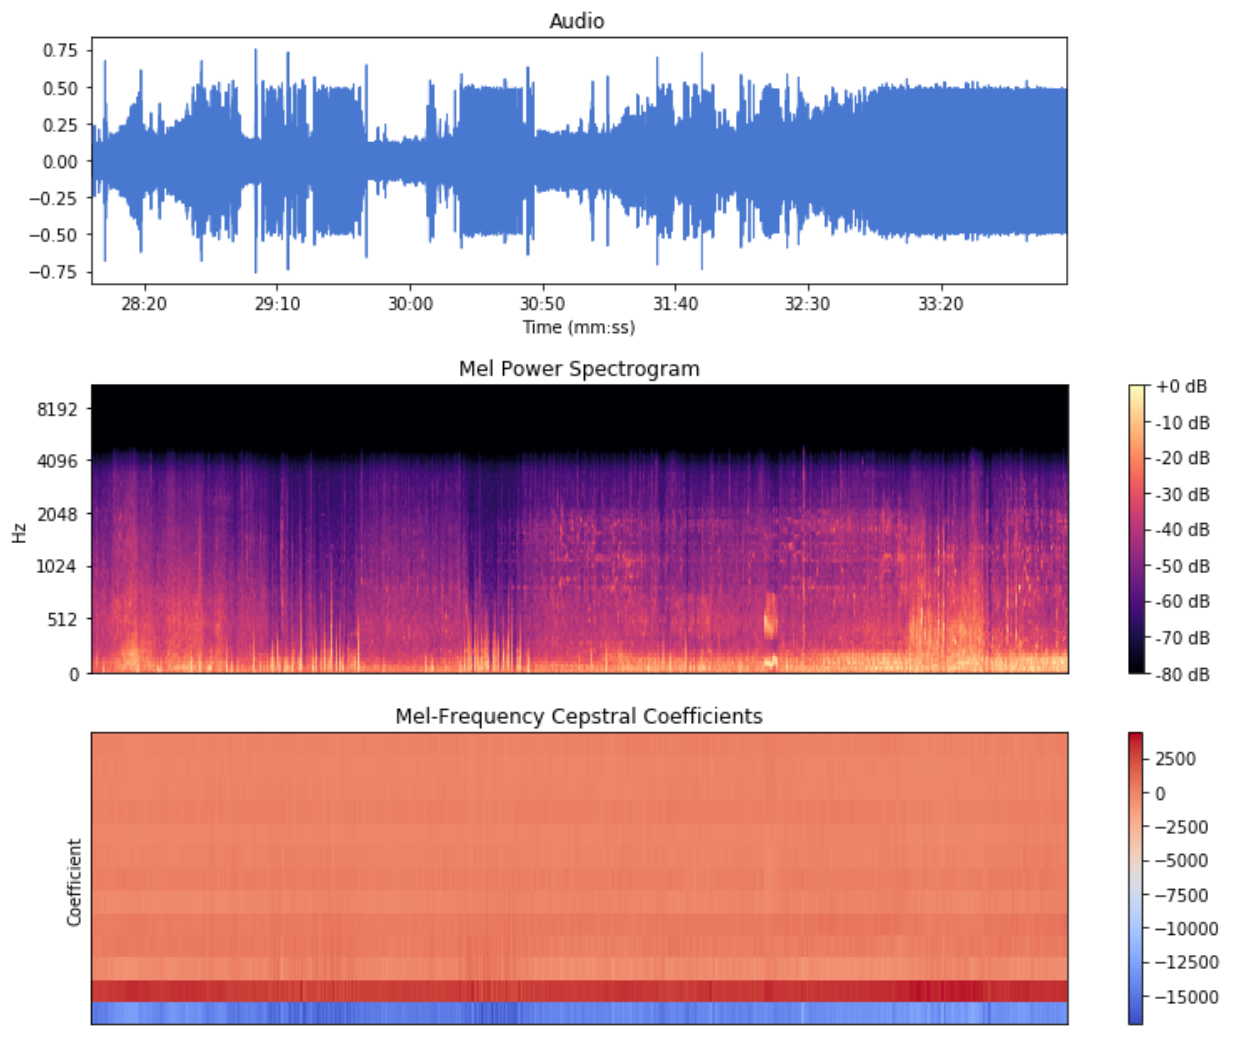
\includegraphics[width=\textwidth]{figures/audio/audio_processing.png}
    \caption{Segment of our audio processing pipeline corresponding to approximately 6 minutes from the `Campus' dataset detailed in \ref{fig:campus-map} (region labels 4,5,6,7). Compared to more traditional problems involving speech or music, obvious changes in the RMS amplitude and power spectrum are relatively subtle and infrequent.}
    \label{fig:audio-pipe}
\end{figure}

By only considering the first $M$ coefficients, we discard the most complex parts of the signal, and preserve only the `spectral envelope', i.e. the general shape of the sound. The higher order coefficients encode more ephemeral aspects of the sound, which in the case of matching ambiences would be detrimental to robustness.
Although the decomposition of an ambient sound's spectrum into envelope and noise (which coefficient is the appropriate boundary for a fundamentally noisy signal?) is much more obscure than that of an instrument or voice, we hypothesize that consistent noise sources such as air conditioners, passing vehicles, and distant vocal chatter are sufficiently distinct to be captured (for example, see Fig.~\ref{fig:audio-pipe}).  The final stage of our feature extractor is quantization via a k-means codebook, similar to the quantized SIFT features in the previous example. With reasonable window size and overlap parameters, this method produces dozens of feature observations per second.

\subsection{Evaluation}

We recorded audio datasets from two trajectories through the McGill campus and surrounding downtown area of Montreal, 51 and 43 minutes long respectively. The audio was recorded in stereo from a commodity hand-held video camera at a 44.1 kHZ sample rate while walking at approximately constant speed, and later combined into a single channel. The trajectories were chosen to contain varied sound environments, and contain both indoor and outdoor sounds, as well as sounds from busy and quiet environments. The maps of these trajectories are shown in Figs.~\ref{fig:campus-map} and~\ref{fig:figure8-map}. The dotted paths segments correspond to indoor environments. The \emph{Four-loops} dataset consists of four loops through the trajectory shown in the map, while \emph{Figure-8} is a trajectory which is topologically equivalent to figure `8', and is looped twice.  

We graphically represent when the trajectory returns to the same place with similarity matrices, where element $(i,j)$ is colored (non-black) if the agent was labelled to be in the same region at time $i$ and $j$, i.e., region labels $r_i = r_j$. For each trajectory, we hand-labelled the region for each temporal window according to the segments shown in Figs.~\ref{fig:campus-map} and~\ref{fig:figure8-map}, giving the similarity matrices seen in Fig.~\ref{fig:campus-groundtruth} and~\ref{fig:figure8-groundtruth}. Thus, colored blocks in the ground truth similarity matrices correspond to sets of locations that belong to a single spatial region with a consistent acoustic profile. For example, the red squares in Fig. \ref{fig:campus-groundtruth} correspond to sets of pairs of points along the trajectory that all have acoustic profiles produced at the roadway marked as region 1 in Fig. \ref{fig:campus-map}. 


\begin{figure}
    \begin{minipage}{0.45\textwidth}
        \subfloat[][]{
            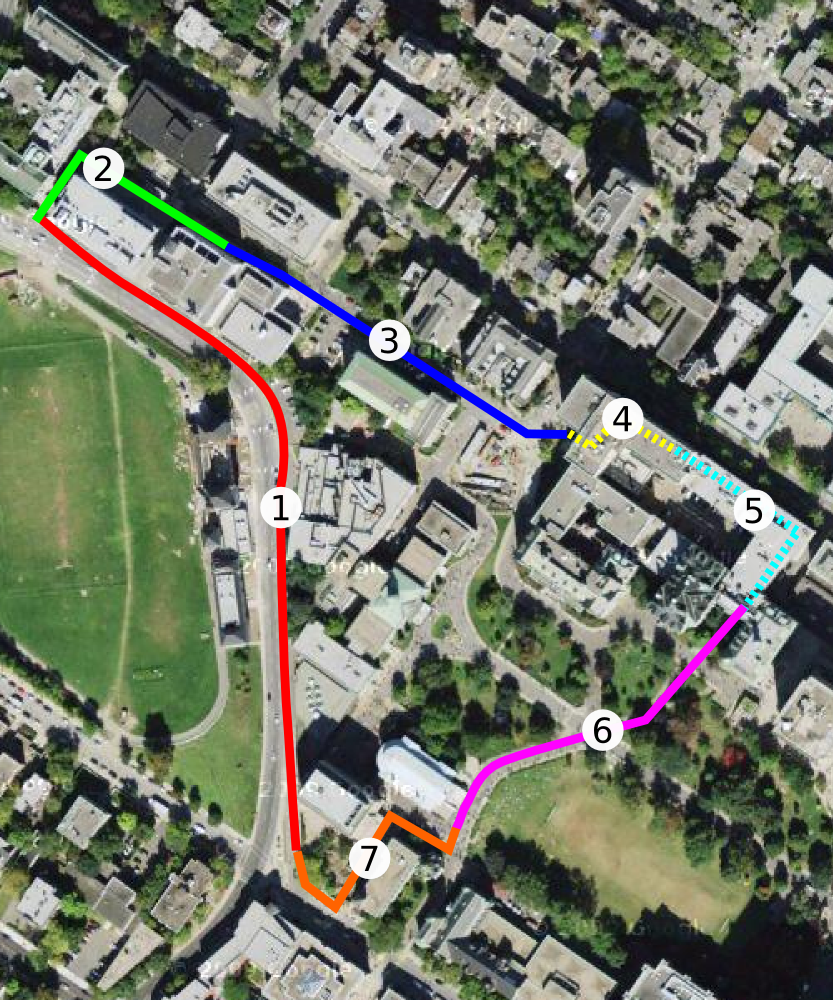
\includegraphics[width=\columnwidth]{figures/audio/campus/campus-map.png}
            \label{fig:campus-map}
        }
    \end{minipage} \hfill
    \begin{minipage}{0.48\textwidth}
        \subfloat[][]{
            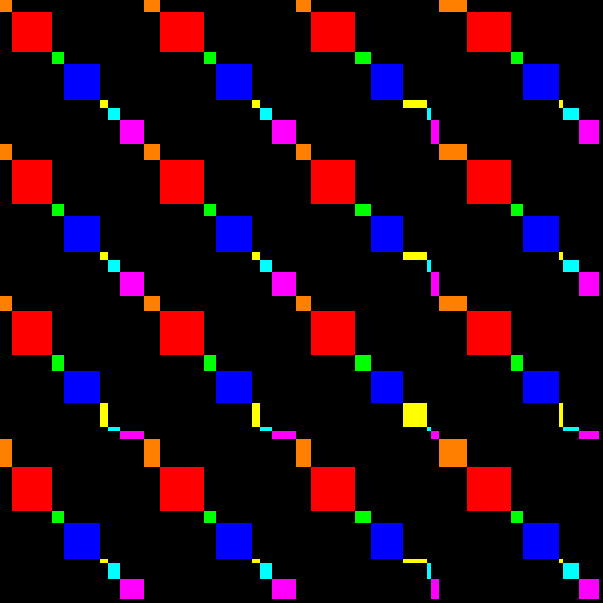
\includegraphics[width=0.45\columnwidth]{figures/audio/campus/groundtruth_color.pdf}
            \label{fig:campus-groundtruth}
        } %
        \subfloat[][]{
            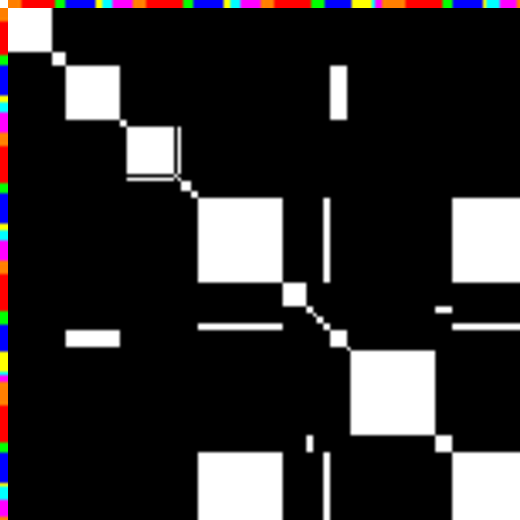
\includegraphics[width=0.45\columnwidth]{figures/audio/campus/dmat_words_campus+margin.pdf}
            \label{fig:campus-words}
        } \\
        \subfloat[][]{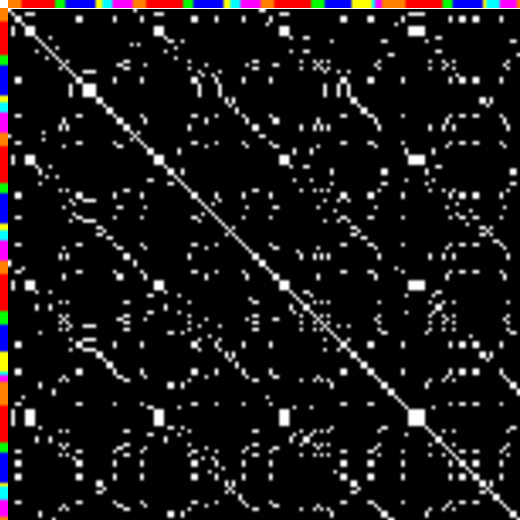
\includegraphics[width=0.455\columnwidth]{figures/audio/campus/dmat_regions_g0_campus+margin.pdf}
        \label{fig:campus-topicsg0}
        } %
        \subfloat[][]{
            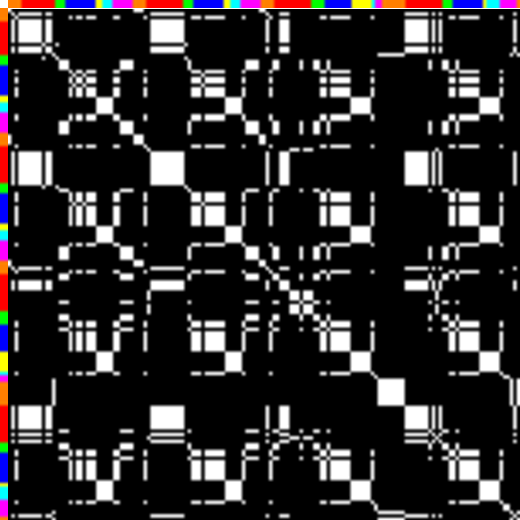
\includegraphics[width=0.455\columnwidth]{figures/audio/campus/dmat_regions_g4_campus+margin.pdf}
            \label{fig:campus-topicsg4}
        }%
    \end{minipage}
    
    \caption{\emph{Four-loops dataset:} 
        \protect\subref{fig:campus-map} Map showing the path traversed while recording the dataset.
        \protect\subref{fig:campus-groundtruth} Ground truth similarity matrix.
        \protect\subref{fig:campus-words} Similarity matrix for feature-based region labelling ($g=12$).
        \protect\subref{fig:campus-topicsg0} Similarity matrix for LDA-topics based region labelling ($g=0$).
        \protect\subref{fig:campus-topicsg4} Similarity matrix for temporally smoothed LDA region labelling ($g=4$).
    }
    \label{fig:dataset-campus}
\end{figure}

\begin{figure}
    \begin{minipage}{0.52\textwidth}
        \subfloat[][]{
            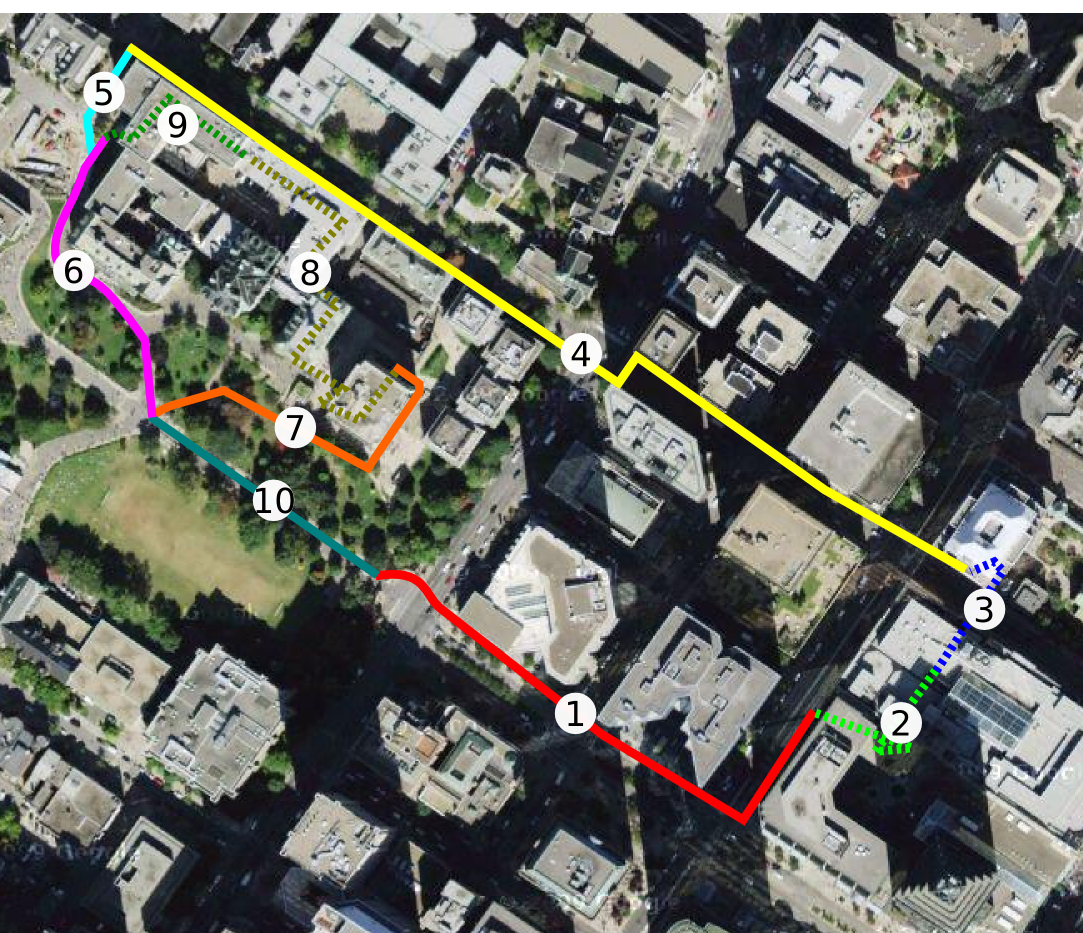
\includegraphics[width=\columnwidth]{figures/audio/figure8/figure8-map.png}
            \label{fig:figure8-map}
        }
    \end{minipage} \hfill
    \begin{minipage}{0.45\textwidth}
        \subfloat[][]{
            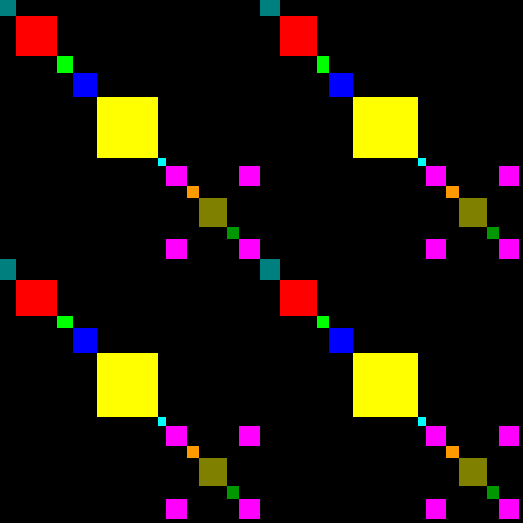
\includegraphics[width=0.46\columnwidth]{figures/audio/figure8/groundtruth_color.pdf}
            \label{fig:figure8-groundtruth}
        } %
        \subfloat[][]{
            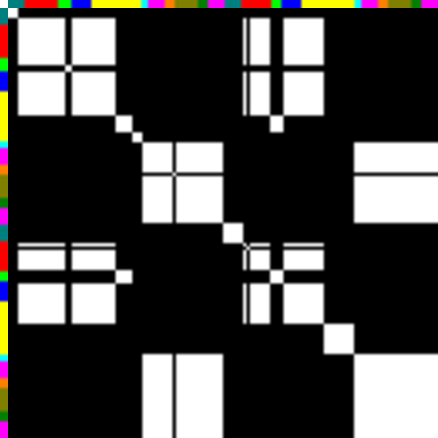
\includegraphics[width=0.46\columnwidth]{figures/audio/figure8/dmat_words_figure8+margin.pdf}
            \label{fig:figure8-words}
        } \\
        \subfloat[][]{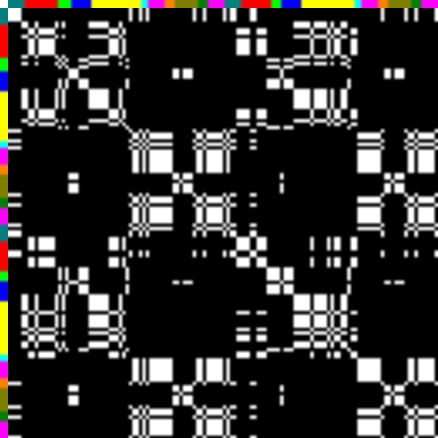
\includegraphics[width=0.46\columnwidth]{figures/audio/figure8/dmat_regions_g0_figure8+margin.pdf}
        \label{fig:figure8-topicsg0}
        } %
        \subfloat[][]{
            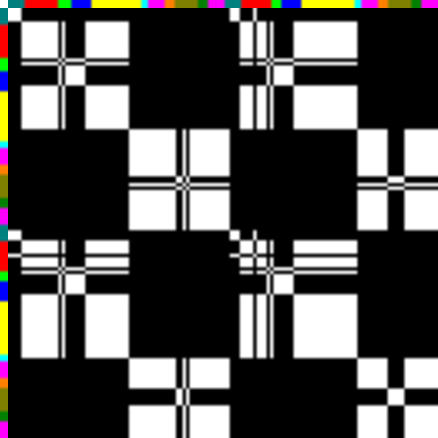
\includegraphics[width=0.46\columnwidth]{figures/audio/figure8/dmat_regions_g2_figure8+margin.pdf}
            \label{fig:figure8-topicsg2}
        }%
    \end{minipage}
    
    \caption{\emph{Figure-8 dataset:} 
        \protect\subref{fig:figure8-map} Map showing the path traversed while recording the dataset.
        \protect\subref{fig:figure8-groundtruth} Ground truth similarity matrix.
        \protect\subref{fig:figure8-words} Similarity matrix for feature-based region labelling ($g=14$).
        \protect\subref{fig:figure8-topicsg0} Similarity matrix for LDA-topics based region labelling ($g=0$).
        \protect\subref{fig:figure8-topicsg2} Similarity matrix for temporally smoothed LDA region labelling ($g=2$).
    }
    \label{fig:dataset-f8}
\end{figure}

The regions were produced by identifying points on the map where environment transitions occur, and were chosen to be geographically relevant rather than acoustically relevant in order to test the hypothesis that these two types of transitions often align. Doorways for entering and exiting buildings as well as the edges of campus were the main landmarks. Some gradual environment transitions occur in the datasets, for instance going from quiet outdoors parts of campus to busy ones. We do not try to capture these gradual transitions in the ground-truth, and instead just pick a single point where this transition occurs, as is in the transition from region 2 to 3 in Fig.~\ref{fig:campus-map}.

We first generated two vocabularies of size 1500 by clustering MFCC features from the two datasets, and then used the vocabulary from the first dataset to generate MFCC words for the second, and vice versa. Each MFCC word corresponds to a 92 millisecond window of the sound, with a 50\% overlap with the previous window. We then grouped these words into windows each representing 20 seconds of sound, with no overlap. The \emph{Four-loops} dataset has 151 such windows, and the \emph{Figure-8} dataset has 128 windows. We ran the temporally smoothed LDA on these datasets, varying the neighborhood size $g$, in number of 20-second windows.

For each window, we then compute the region label $r_t$ by counting the most popular topic label in that window. Then, for each pair of windows, we compare the corresponding region labels, and mark the corresponding times to belong to the same region if the region labels match. 

We experimented with neighborhoods of $g=0 \ldots 10$ windows, and computed the true positive rates (TPR) and false positive rates (FPR) resulting from comparison with the ground truth matrix. TPR refers to the fraction of true positive similarity matches out of all positive results returned by the algorithm. Similarly, FPR refers to the fraction of false positive similarity matches out of all negative matches returned by the algorithm. An ideal algorithm has TPR of 1.0 and FPR of 0.0. The resulting plots of TPR vs FPR (known as a Receiver Operating Characteristic, or ROC, curve) are shown in Fig.~\ref{fig:audio-roc-top1}. Figs.~\ref{fig:campus-topicsg4} and~\ref{fig:figure8-topicsg2} show the similarity matrices with the best performance, chosen by their distance from the baseline performance on the ROC curve.  Fig.~\ref{fig:campus-topicsg0}, \ref{fig:figure8-topicsg0} show the similarity matrix for neighborhood size $g=0$, which is equivalent to a standard LDA topic model, where windows are assumed to be independent. This case is the leftmost point on the ``topics'' ROC curve. 

In addition to computing the region assignment through our topic model, we also computed generated region labels directly from the window feature distributions. This model assigns the region label to be the index of the most common feature in that window's neighborhood. We varied neighborhood sizes for the direct region labelling approach, using the same set of neighborhood sizes as we did for the topic model. The similarity matrices for the best performing neighborhood size setting are shown in Figs.~\ref{fig:campus-words} and~\ref{fig:figure8-words}.

\begin{figure}
\begin{center}

\subfloat[]{
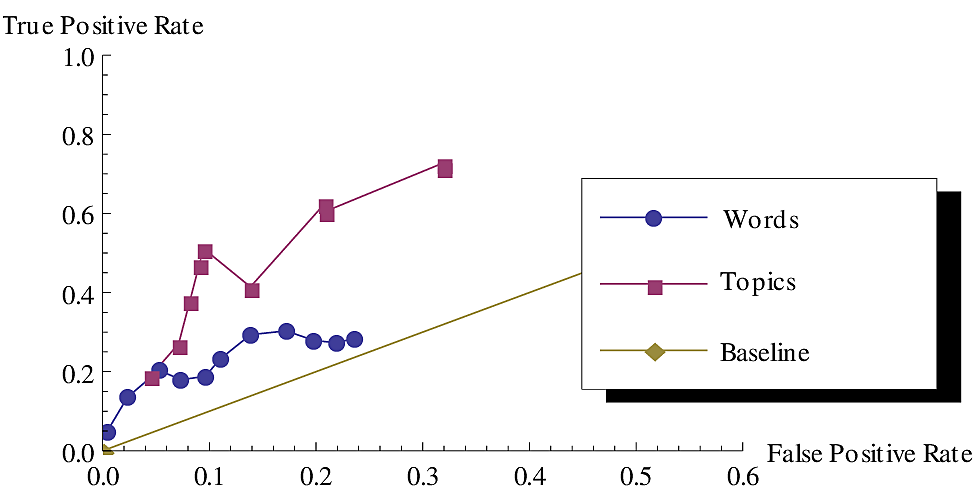
\includegraphics[width=0.48\linewidth]{figures/audio/campus/roc_top1_words_topics}
\label{fig:audio-roc-top1-campus}
}
\subfloat[]{
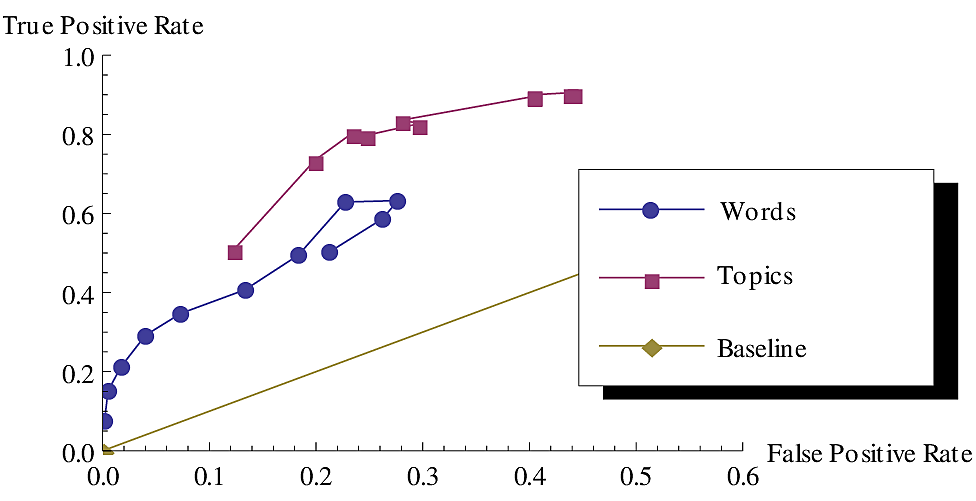
\includegraphics[width=0.48\linewidth]{figures/audio/figure8/roc_top1_words_topics}
\label{fig:audio-roc-top1-figure8}
}

\caption{ \emph{ROC curves for same-place recognition based on ambient sound:}
\protect\subref{fig:audio-roc-top1-campus} Four-loops dataset.
\protect\subref{fig:audio-roc-top1-figure8} Figure 8 dataset.
}
\label{fig:audio-roc-top1}
\end{center}
\end{figure}

Our experiments indicate that the temporal topic model finds a representation where a simple region assignment is much more meaningful than directly considering the features or using a topic model without any temporal considerations. Fixing the false positive rate to be less than 0.25, Table \ref{tab:audio-results-summary} shows the best detection accuracy for each algorithm for both the datasets. It should be noted that the reported false positive rate is probably higher than the actual false positive rate because similar sounding regions at physically different locations were marked as distinct in our ground truth. For example, regions (1) and (4) from the \emph{Figure-8} dataset are both recorded from busy streets, and sound the same, and as result are detected to be the same region by the proposed algorithm (Fig. \ref{fig:figure8-topicsg2}). From the similarity matrices produced by the system for the two datasets (Fig. \ref{fig:campus-topicsg4}, \ref{fig:figure8-topicsg2}), we can see that the algorithm is successfully able to detect loop closure at many, but not all locations.

In both datasets, the temporally smoothed topic-based region labels outperformed the top-word-based region labels. Further, the topic model with temporal independence of windows (the leftmost point in the topics line) does not significantly outperform the naive feature-based approach. This indicates how critical it is to explicitly model the dependencies between adjacent observations. To reiterate, we do not require topics to explicitly correspond to particular real-world regions. Yet in order to find a self-consistent region labelling where returning to the same location means our model will produce the same label we still must consider the temporal smoothness of region labels.

\begin{table}
    \centering
    \begin{tabular}{|c|c|c|c|c|c|c|}
    \hline
    Dataset & \multicolumn{6}{|c|}{Best Detection Accuracy}\\
    & \multicolumn{6}{|c|}{(False positive rate $<$ 0.25)}\\ \cline{2-7}
    &\multicolumn{2}{|c|}{MFCC-words}& \multicolumn{2}{|c|}{LDA}&\multicolumn{2}{|c|}{Temp. Smooth. LDA}\\
    \hline
    &TPR& FPR&TPR& FPR&~~ TPR ~~& FPR\\
    \hline
    Four-loops & 0.29 &0.15 & 0.19 & 0.04 & 0.61 & 0.21\\
    \hline
    Figure-8 & 0.63 & 0.23 & 0.50 & 0.12 & 0.80 & 0.23\\
    \hline
    \end{tabular}
    
    \caption{Best accuracy of unsupervised same place recognition from ambient sound.}
    \label{tab:audio-results-summary}
\end{table}

\todo{really nice. bravo!}
%!TEX root = thesis.tex

\chapter{Combining topics and domain expertise to develop insight into plankton ecology} \label{ch:plankton}

As we have seen, the spatio-temporal topic model is a powerful model for unsupervised classification of location specific data, and by carefully defining a feature function, we can achieve intuitive classifications that match human semantic annotations. However, our interpretation of the model's outputs has thus far been somewhat straightforward. In this chapter, we delve deeper into how topic models can be used for tasks beyond classification.

A key feature of the spatio-temporal topic model is that it excels at finding co-occurrences in data that can be explained by the region in which each observation occurred. In addition to leading to appealing maps, this property means that topic distributions are often easier to predict accurately than other non-smooth representations of a dataset. Further, given a predicted topic distribution and the topics themselves, the maximum likelihood feature distribution is trivial to produce.

In this chapter, we explore two approaches that take this approach to predict unobserved feature distributions. Our motivation is to develop methods that provide intuitive insight into scientific data. In these applications, it is important for models to act in concert with domain knowledge, and therefore, it is crucial that insights be in terms of observable data, rather than abstract topic representations. As we will show, by predicting the data through the spatio-temporal topic model we enable representations that make intuitive trends in the data evident, and thus directly suggest questions for further study.

\section{Phytoplankton community model}
In addition to contributions to the machine learning literature, in the work presented in this chapter, we aim to contribute to domain research in phytoplankton ecology. Phytoplankton are microscopic organisms that form the base of marine food webs. They produce chlorophyll and other pigments to harvest sunlight and fuel photosynthesis, so they can utilize $\mathrm{CO}_2$ and other nutrients to produce $\mathrm{O}_2$ and new organic matter. As such, they play critical roles in global biogeochemical cycles and in structuring marine ecosystems.  
Marine scientists have long used techniques to measure the amount of chlorophyll in a water sample as a proxy for phytoplankton biomass \citep{Lorenzen1966}. These methods are coarse and give only bulk indices, with no information about which species of phytoplankton are present. Phytoplankton are extremely diverse, however, and their community structure plays a major role in shaping ecosystems and their functions. As an extreme example, particular species are known to cause toxic blooms that can threaten wildlife as well as human health.

\begin{figure}
\begin{center}

\subfloat[]{
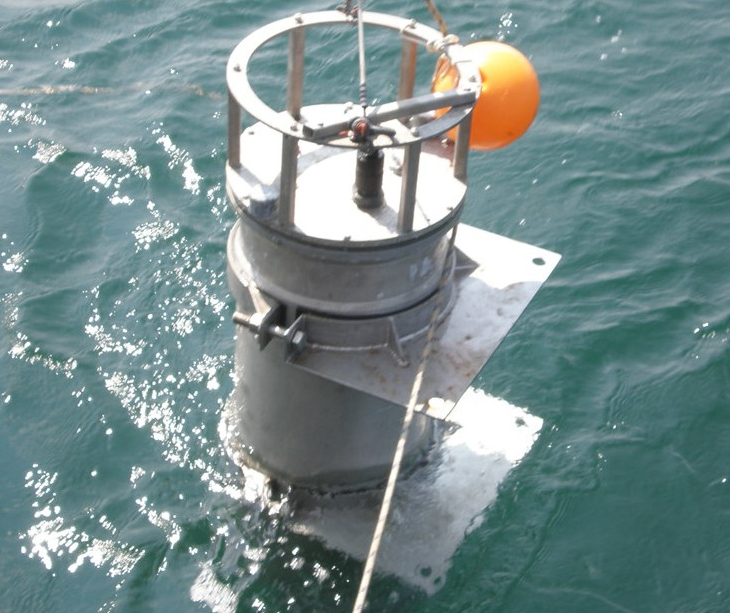
\includegraphics[width=0.45\columnwidth]{figures/oceans/IFCB.jpg}
\label{fig:ifcb-device}
}%
\subfloat[]{
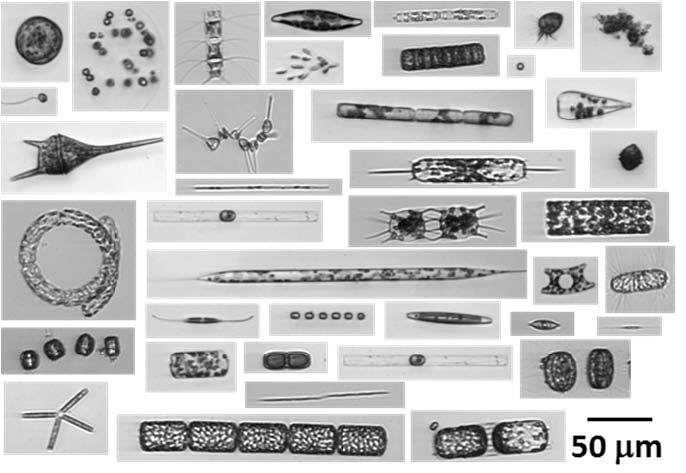
\includegraphics[width=0.54\columnwidth]{figures/icra_plankton/IFCB_collage.jpg}
\label{fig:ifcb-collage}
}
\end{center}
\caption{
\protect\subref{fig:ifcb-device} Imaging FlowCyto Bot (IFCB) being deployed at Martha's Vineyard, MA.
\protect\subref{fig:ifcb-collage} Example phytoplankton detections from IFCB.
}
\label{fig:ifcb}
\end{figure}

To meet the gap in observational capability that includes taxonomic resolution, Sosik and Olson have developed the automated, submersible Imaging FlowCytobot (IFCB, Fig.~\ref{fig:ifcb-device})~\citep{Olson2007a}. IFCB acts as an autonomous underwater microscope, collecting water samples and imaging small droplets at high resolution ($\sim$\SI{1}{\micro\meter}). The coupled analysis system \citep{Sosik2007} is able to detect and crop phytoplankton within these images (See Fig.~\ref{fig:ifcb-collage}). Many of these contain sufficient detail to be automatically classified to the genus or species level by a random-forest based system \citep{Sosik2016}. IFCB is designed to serially sample ocean water and perform detection and classification for long periods of time (weeks to years) with minimal manual intervention.

Sosik, Olson, and other IFCB users have collected impressively detailed datasets of plankton taxon (\emph{ie.} species or genus) abundance, both with long-term fixed location IFCB deployments, and over large areas by deploying IFCB underway on a ship.\footnote{Available online at \url{http://ifcb-data.whoi.edu/mvco/}}
Nevertheless, this detail comes at the price of intuitive, comprehensive models using classic statistical techniques. To our knowledge, no other work has attempted to derive understanding about the interactions between multiple taxa in this dataset, nonetheless all of them considered at once.

We hypothesize that by taking sparsity and spatio-temporal smoothness into account, a spatio-temporal topic model will be able to produce such an account without sacrificing interpretability. Specifically, the topic model's discrete-valued feature function is taken to be the occurrence of each taxon, and neighborhoods are taken to be the temporal or spatio-temporal windows in which the observations were made by IFCB. We interpret the resulting word-topic distributions as `communities' -- probabilistic groupings of plankton taxa that tend to co-occur. Under this interpretation, the topic-neighborhood distributions describe the mixture of communities found in a given location.

Similar to previous examples in this thesis, we expect that each community should be mainly comprised of only a few taxa, that for any location few communities should be present, and that within some neighborhood the distribution of communities should be similar. By applying priors which prefer models that respect these conditions, we ensure that our community model will be not only accurate, but also easy to interpret.  As we have seen, the (spatio-) temporal topic model can be used to estimate the posterior probability of topic assignments $P(\boldsymbol{z} | \boldsymbol{w})$ via the collapsed Gibbs sampler update (in Eqn.~\ref{eqn:posterior}), and further that given a set of topic assignments, the posterior distributions for $\Theta$ and $\Phi$ are given by $Dir(\alpha + \boldsymbol{N}_{g(x)}^{1:K})$ and $Dir(\beta + \boldsymbol{N}_k^{1:V})$ respectively. The mean of a Dirichlet distribution is its parameter normalized, so the maximum likelihood values, denoted $\hat{\Theta}$ and $\hat{\Phi}$ are trivial to recover

\begin{equation} \label{eqn:mle_thetaphi}
\hat{\Theta}_{g(x), k} = \frac{N^k_{g(x)} + \alpha}{\sum_{j=1}^K N^j_{g(x)} + \alpha}, \quad
\hat{\Phi}_{k,w_i} = \frac{N^{w_i}_k + \beta}{\sum_{v=1}^V N^v_k + \beta},
\end{equation}

To tie our communities back to the domain of phytoplankton observations, we consider learning the community model, but also additional means of estimating the MLE community distributions when the phytoplankton observations themselves are not available. Supposing we have some method to estimate of these community distributions $\check{\theta} \approx \hat{\theta}$, we can in turn estimate the distribution of phytoplankton taxa
\begin{equation} \label{eqn:word-estimate}
P(w = v | \theta, \Phi) = \sum_{k=0}^K \theta_k \Phi_{k,v} \approx \sum_{k=0}^K \check{\theta}_k \hat{\Phi}_{k,v}
\end{equation}

A final issue in the formulation of our phytoplankton community model is that because these datasets are so unique, to our knowledge no domain research has attempted to define phytoplankton communities, and therefore we do not have strong information about how to set the number of topics $K$. For this reason, instead of fixing $K$ ahead of time, we apply a Dirichlet process (DP) prior on $\theta$ and learn the number of topics from data following the Bayesian non-parametric approach of \citep{Girdhar2016}, (BNP-ROST).

The DP is an infinite-dimensional generalization of the Dirchlet distribution, often used as a prior for infinite mixture models, where the number of components is not known \emph{a priori}. It is parameterized by a probability distribution $G$ with support set $A$, and a positive, real-valued scale parameter $\eta$. It is defined by the property that any finite partition of $A$ (a disjoint, covering set of subsets) is jointly Dirichlet distributed, \emph{ie} for all finite partitions $\{A_0, \ldots, A_r\}$ \citep{Teh2010}
\begin{equation}
H \sim DP(\eta, G) \Rightarrow (H(A_0), \ldots, H(A_r)) \sim Dir(\eta G(A_0),\ldots,\eta G(A_r))
\end{equation}
In the Bayesian non-parametric topic model, a DP prior is placed on $\theta$. $A$ is considered to be the set of possible topic assignments for a word, with no limit on the maximum possible value. The key insight is that for any number of topics currently in use, $K$, the distribution over the partition with an element for each of the $K$ topics, plus another for any other possible topic assignment, \emph{ie.} the partition $\{z = 0, z = 1, \ldots, z = K - 1, z \geq K\}$, is a (finite) Dirichlet. We can view this in terms of the `Chinese Restaurant Process' construction, reparameterizing $G$ and $\eta$ in terms of our original symmetric Dirichlet parameter $\alpha$ and the probability $\gamma$ of incrementing the number of topics \citep{jordan2005}. This interpretation leads to a predictive distribution which is only a minor modification from the Dirichlet predictive distribution (Eqn.~\ref{eqn:posterior}):
\begin{equation}
\begin{aligned}
P(z_i = k | \boldsymbol{z_{-i}}) =
\begin{cases}
\frac{(N^k_{g(x)} + \alpha)}{\gamma + \sum_{j=1}^K N^j_{g(x)} + \alpha} & \mathrm{if}~k < K\\
\frac{\gamma}{\gamma + \sum_{j=1}^K N^j_{g(x)} + \alpha} & \mathrm{if}~k = K
\end{cases}
\end{aligned}
\end{equation}

\section{Learning communities that are explained by the environment} \label{sec:plankton-seasonal}
Our first study involving IFCB plankton data aims at learning an interpretable community model for a fixed-location deployment at Martha's Vineyard Coastal Observatory (MVCO), one mile off the south-shore of Martha's Vineyard, MA \citep{Kalmbach2017}. In addition to an IFCB, MVCO has a suite of other sensors, enabling inquiry into the relationships between phytoplankton abundance and environment variables including oceanographic and meteorological factors such as dissolved $\mathrm{0}_2$ content, salinity, air and water temperature, and rainfall. While the combination of these two data sources could be used as the basis to learn intricate models of the precise relationship between each taxon and the environment, in this work we show that by first accounting for the associations between taxa, our method can capture most of the same information while requiring minimal domain knowledge.

We propose to use a simple simple linear-ridge regressor to predict the distribution of phytoplankton taxa from environment variables. We first train the community model and compute the MLE estimates $\hat{\Theta}$ and $\hat{\Phi}$. Because of the prior imposed by our model, $\hat{\Theta}$ is relatively low-dimensional, sparse, and temporally smooth in comparison to the full phytoplankton distributions. Therefore, we hypothesize that estimating the communities and predicting the phytoplankton taxa by Eqn.~\ref{eqn:word-estimate} will produce more reliable predictions than a direct regression technique.

 In addition, this regression task provides complementary feedback to the topic model, ensuring that the final community model is interpretable in addition to accurate. For this application, instead of using the probability of held-out data as the cross-validation metric, we propose to use the agreement ($1/D_{KL}$) between the predicted taxon distributions and the ground-truth taxon distribution. By doing so, we ensure that the maximum likelihood taxon distributions given the topics closely resemble the true taxon distributions, but also that the topic distributions themselves can be explained simply in terms of the chosen environment variables. For this reason, rather than choosing a complex regression model, which may have better overall performance on the final predictions, we take an unsophisticated linear ridge approach to regression.

\subsection{Martha's Vineyard multi-year timeseries experiment}
We demonstrate our method on a dataset recorded continuously from Jan. 2009 to Jul. 2016 at MVCO. IFCB was configured to automatically sample from 5 ml of surface seawater approximately every 20 min. The classification system generated an average of over 1100 observations per day, distributed over 47 taxa (Fig.~\ref{fig:plankton-mvco-gt}).

We aggregated the observations to produce the taxon distribution for each day during the 7.5 year period, and used this as input to our method. For the regression model, we chose a suite of 18 environment variables from the MVCO ocean data and meteorological data summaries (Fig.~\ref{fig:plankton-mvco-regression-inputs}). In addition to being naively chosen, the environment data features significant gaps and systematic noise due to the practical challenges of long-term ocean sensor deployments. Much of the systematic noise was suppressed by rejecting outliers based on the median absolute deviation of each variable, yet the regression task remains extremely challenging.

% \begin{figure}
%     \centering
%     \begin{subfloat}
%         \centering
%         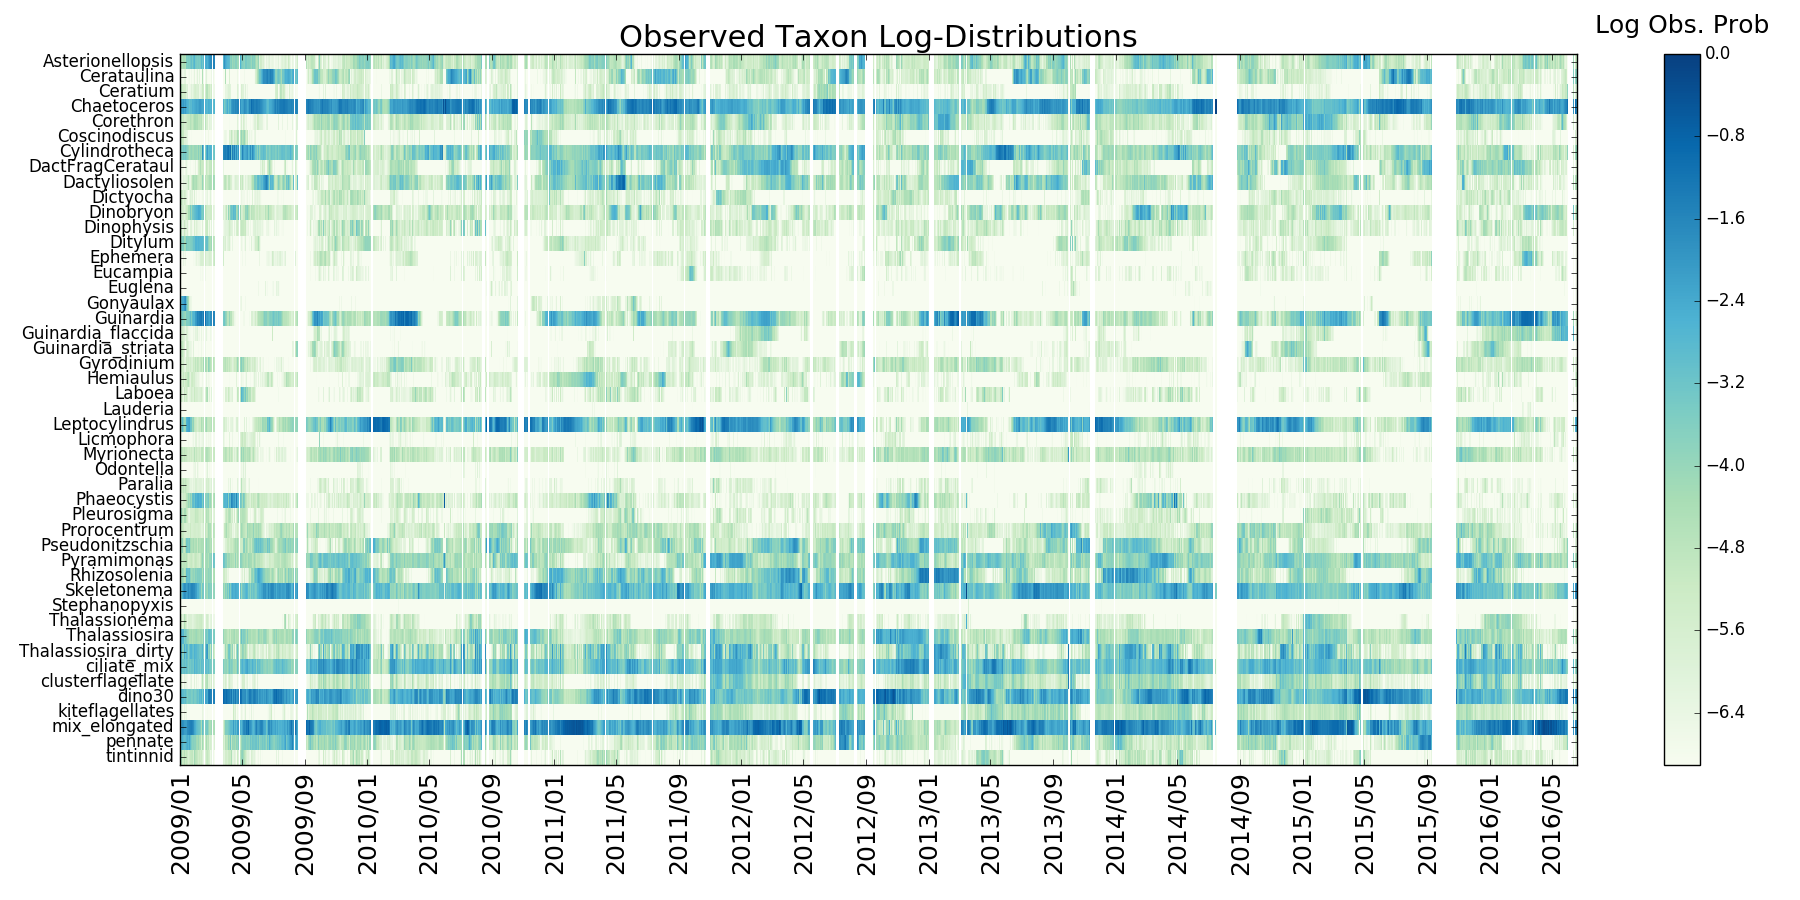
\includegraphics[width=1.\textwidth]{figures/oceans/taxa_distros_gt.png}
%         \caption{Observed daily taxon log-distributions at Martha's Vineyard Coastal Observatory over 7.5 years.}
%         \label{fig:plankton-mvco-gt}
%     \end{subfloat}%
%     \begin{subfloat}
%         \centering
%         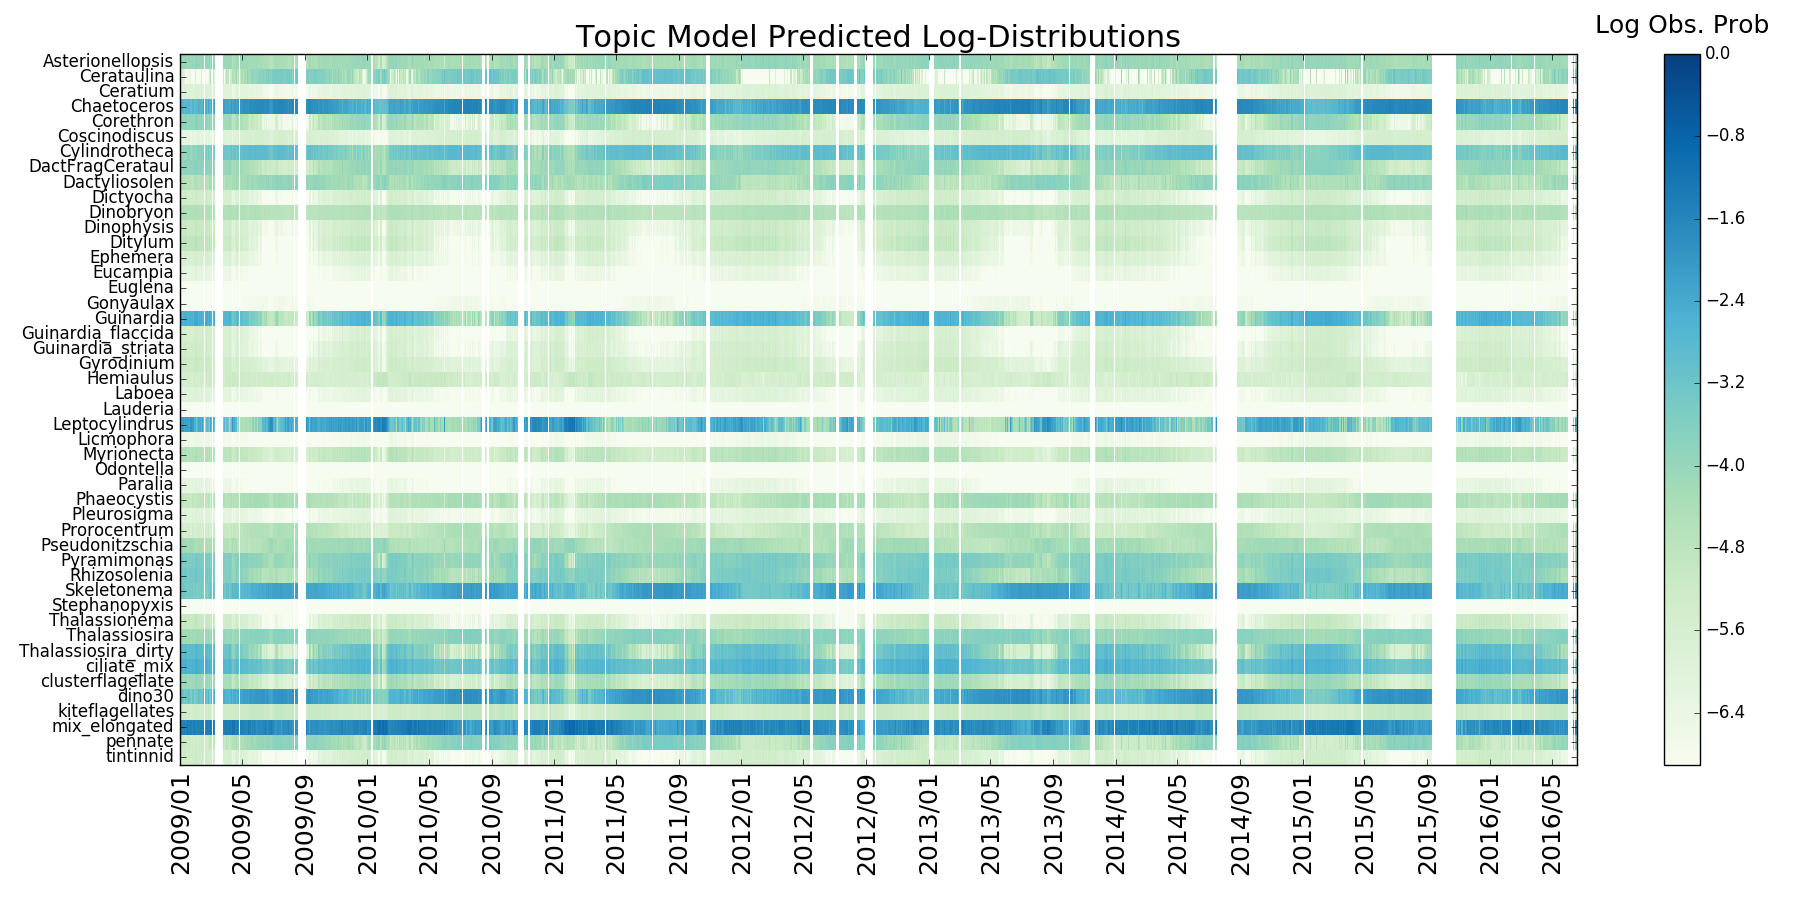
\includegraphics[width=1.\textwidth]{figures/oceans/taxa_distros_hat_topics.png}
%         \caption{Predicted taxon log-distributions using our community model and regression system.}
%         \label{fig:plankton-mvco-topic-est}
%     \end{subfloat}%
% \end{figure}
% \begin{figure}
% 	\ContinuedFloat
%     \begin{subfloat}
%         \centering
%         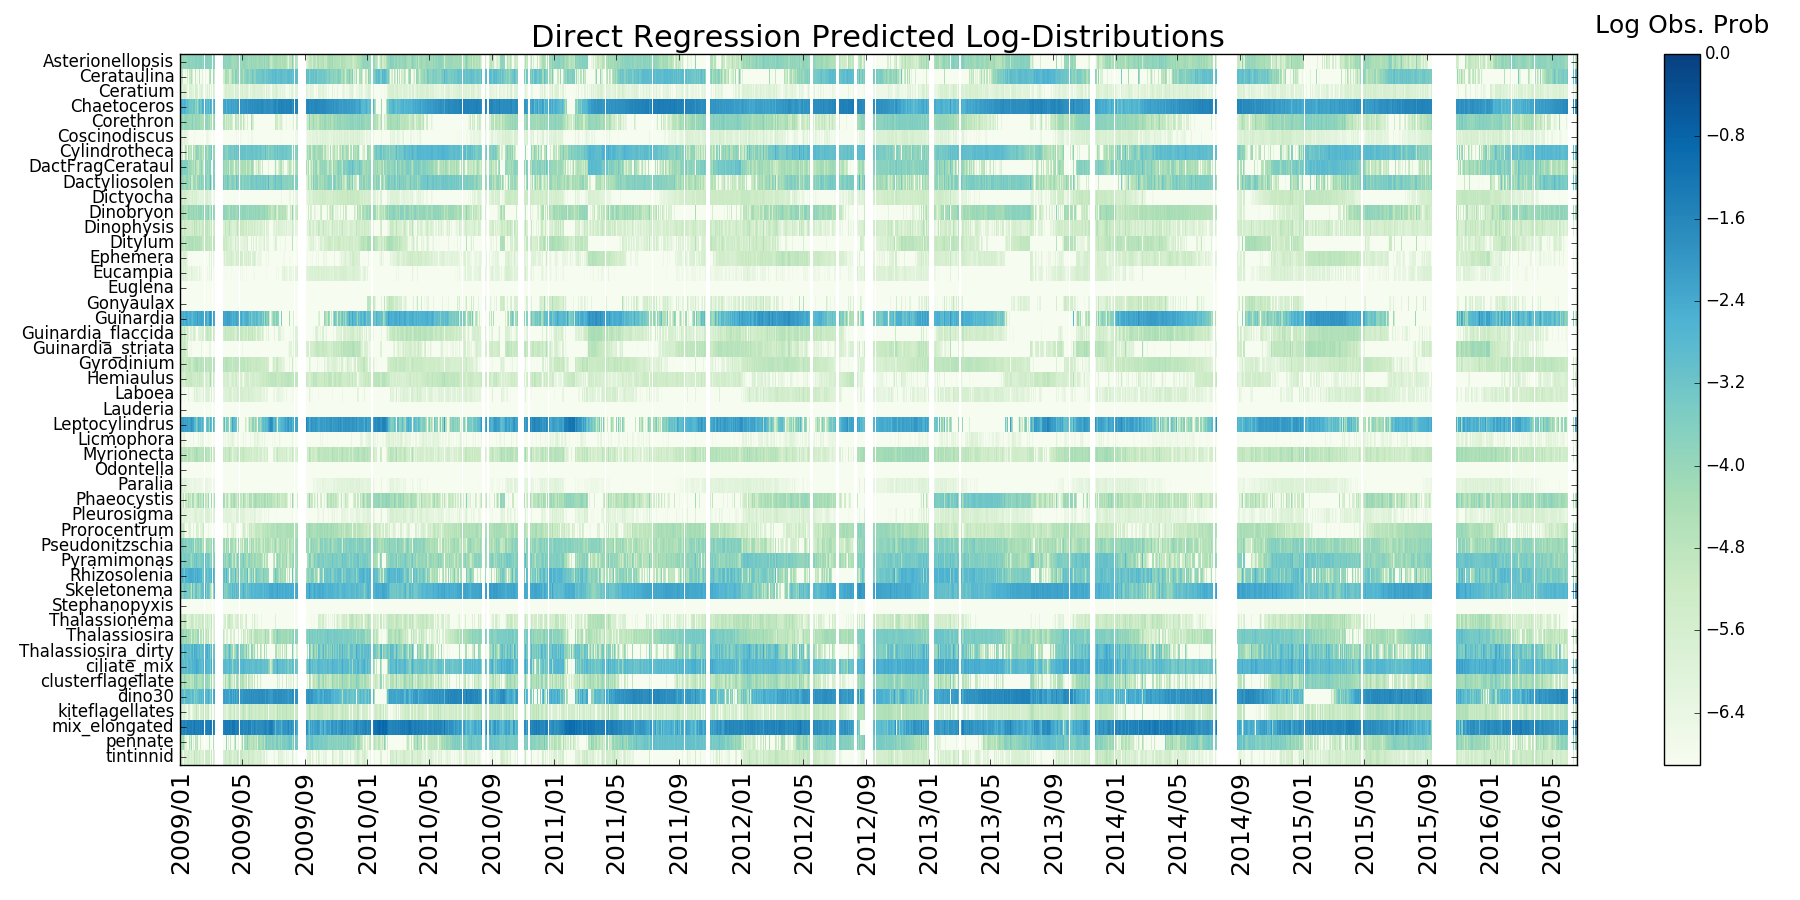
\includegraphics[width=1.\textwidth]{figures/oceans/taxa_distros_hat_words.png}
%         \caption{Predicted taxon log-distributions using direct regression on taxon distributions.}
%         \label{fig:plankton-mvco-word-est}
%     \end{subfloat}
%     \caption{}
%     \label{fig:plankton-mvco}
% \end{figure}

\begin{figure}
    \centering
    \subfloat[][]{
        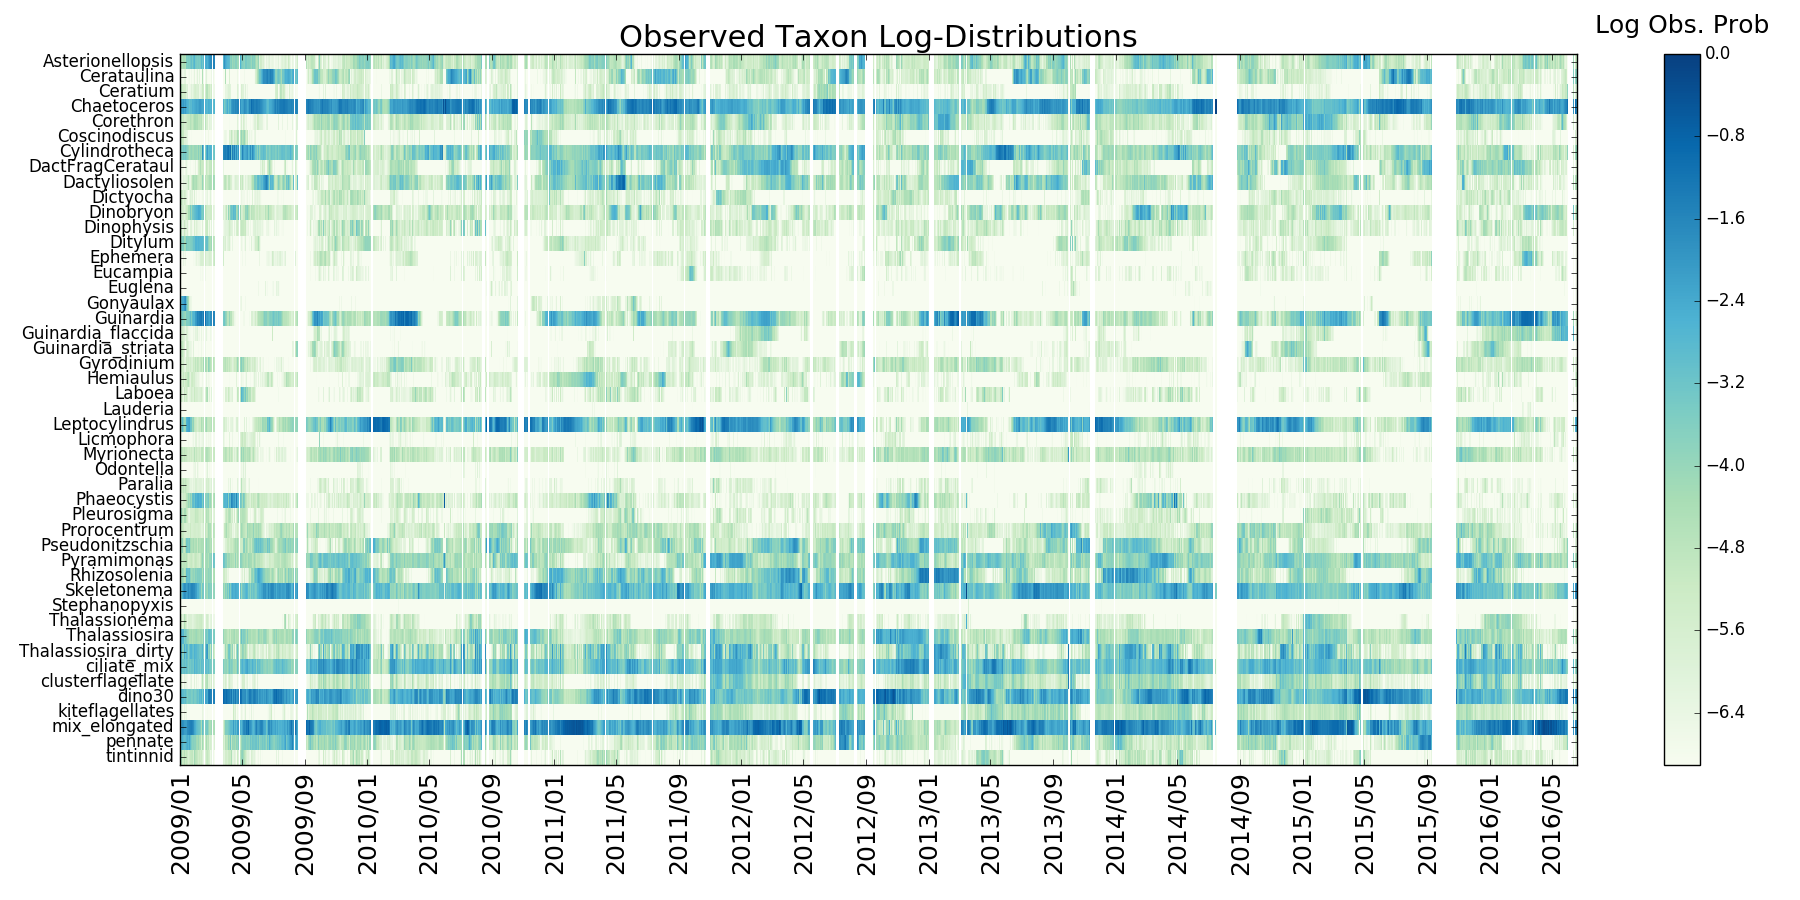
\includegraphics[width=0.8\textwidth]{figures/oceans/taxa_distros_gt.png}
        \label{fig:plankton-mvco-gt}
    }\\
    \subfloat[][]{
        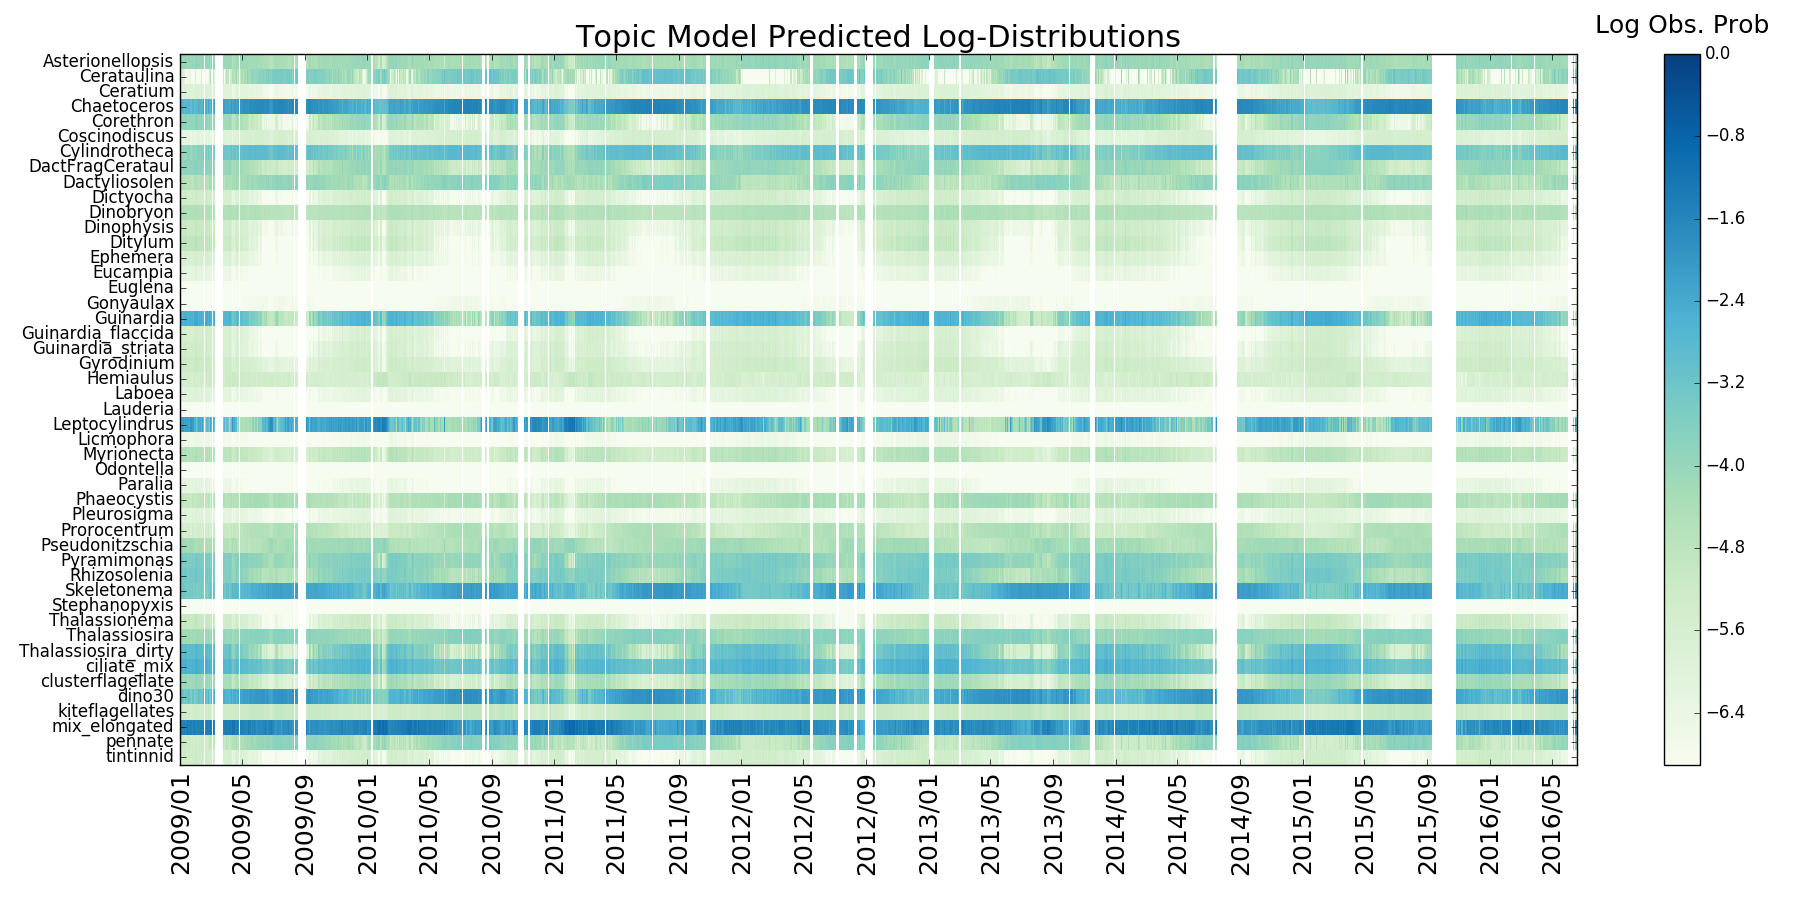
\includegraphics[width=0.8\textwidth]{figures/oceans/taxa_distros_hat_topics.png}
        \label{fig:plankton-mvco-word-est}
    }\\
    \ContinuedFloat
    \subfloat[][]{
        \centering
        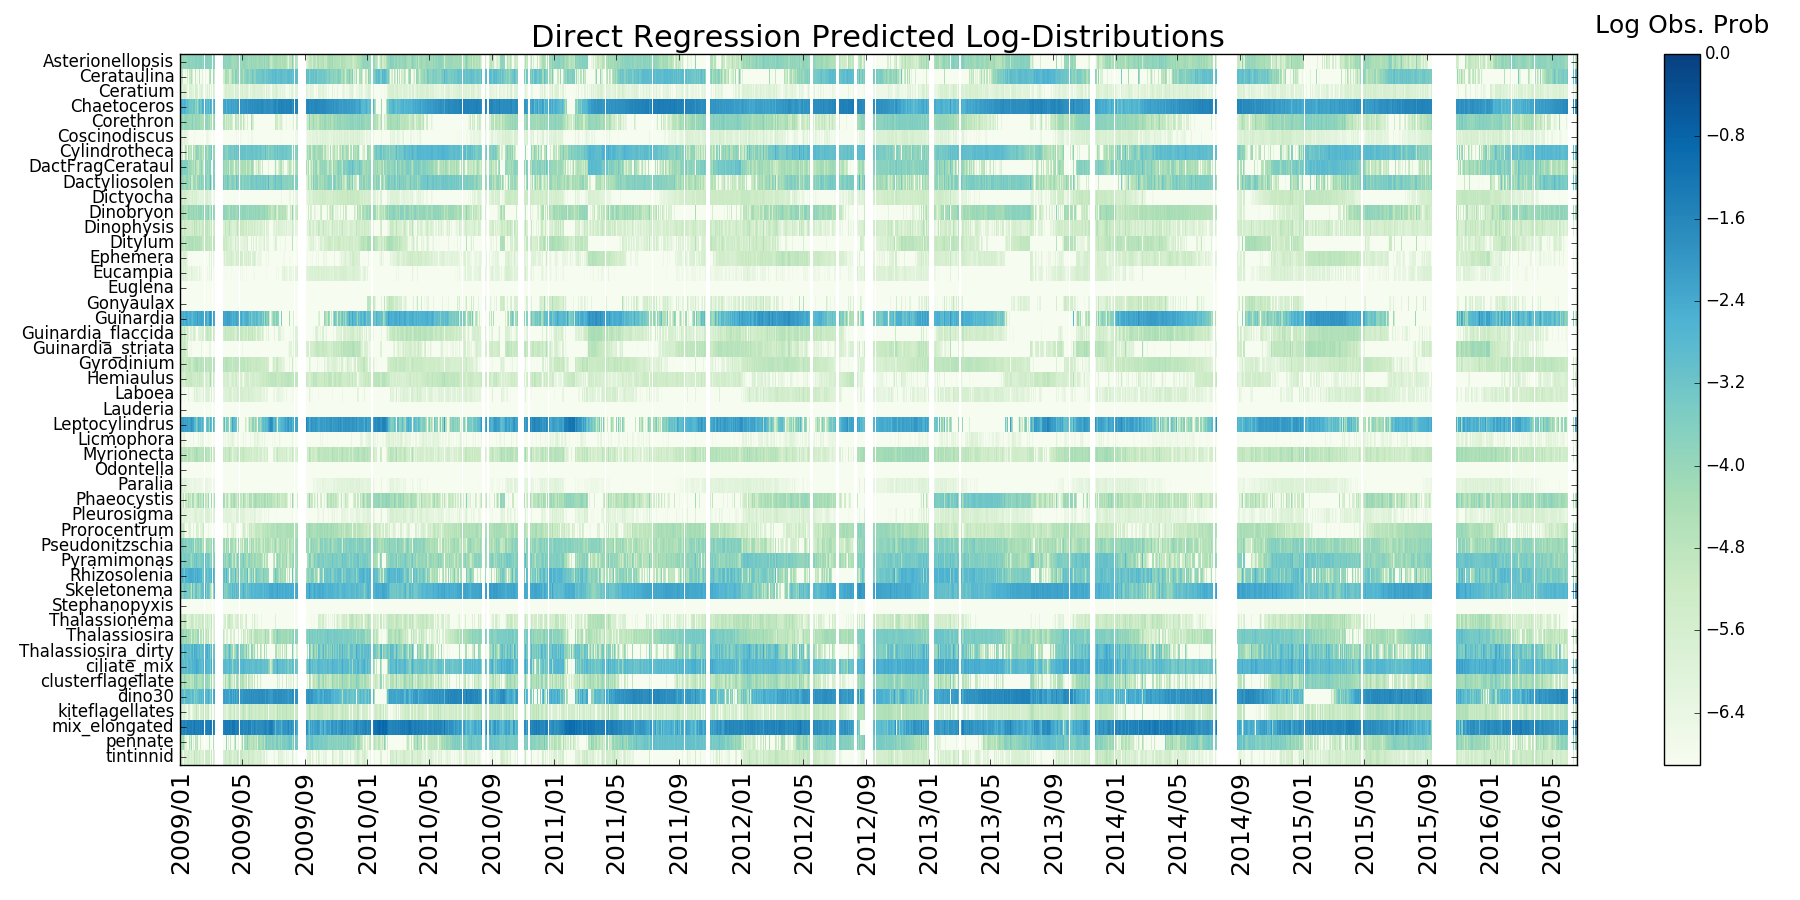
\includegraphics[width=0.8\textwidth]{figures/oceans/taxa_distros_hat_words.png}
        \label{fig:plankton-mvco-topic-est}
    }
    \caption{Taxon log-distributions at Martha's Vineyard Coastal Observatory over 7.5 years.
            \protect\subref{fig:plankton-mvco-gt} Measured.
            \protect\subref{fig:plankton-mvco-word-est} Predicted based on observed maximum likelihood communities.
            \protect\subref{fig:plankton-mvco-topic-est} Predicted based on environmental conditions using our communities-based regression system.
    }
    \label{fig:plankton-mvco}
\end{figure}

\begin{figure}
    \centering
    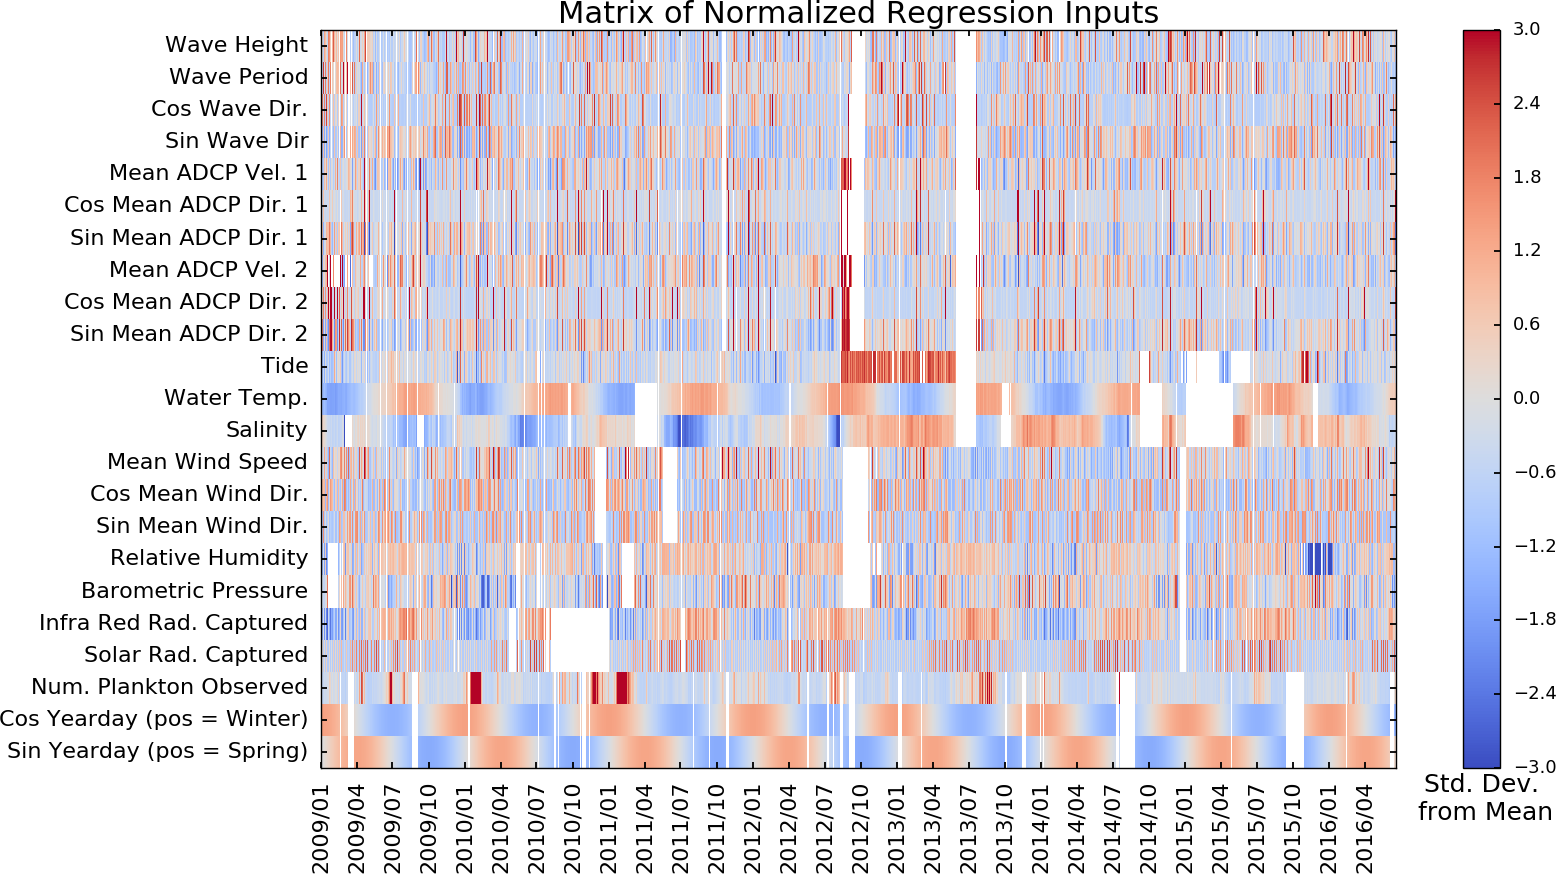
\includegraphics[width=0.9\textwidth]{figures/oceans/RegressionInputsNorm.png}
    \caption{\emph{Environment variables used to predict phytoplankton distributions}:
    Oceanographic and meteorological factors potentially related to phytoplankton life-cycles, centered and scaled to a normal distribution as our regression system receives them. White spaces indicate gaps in the data or where outlier data was removed.}
    \label{fig:plankton-mvco-regression-inputs}
\end{figure}

We trained our community model on the taxon distributions over the entire period multiple times for different hyperparameter settings, varying the topic concentration $\alpha$, the topic-prior concentration $\beta$, the DP prior parameter $\gamma$, and the neighborhood size $g$. For each community model corresponding to a different combination of choices of these hyperparameters, we trained the regression model 8 times, once using each year as the test set and the other 6.5 years for training. Within each training set, we chose the regularization parameter for ridge regression using hold-one-out cross validation. Finally, we used the resulting regressors to predict the respective held-out community distributions for each year, and used the respective community models to predict the taxon distributions.

We demonstrate the utility of our method in comparison to two more standard regression techniques. The first is to predict the taxon distributions directly with a similar ridge regression model and training procedure. The second is to first take a PCA decomposition of the taxon count data, using the first $K$ principle components, where $K$ is the same as the number of communities used by our model, and then use the same ridge regression model and training procedure to predict the PCA weights, and finally project the weights back to predict the taxon distributions.

\begin{figure}
    \centering
    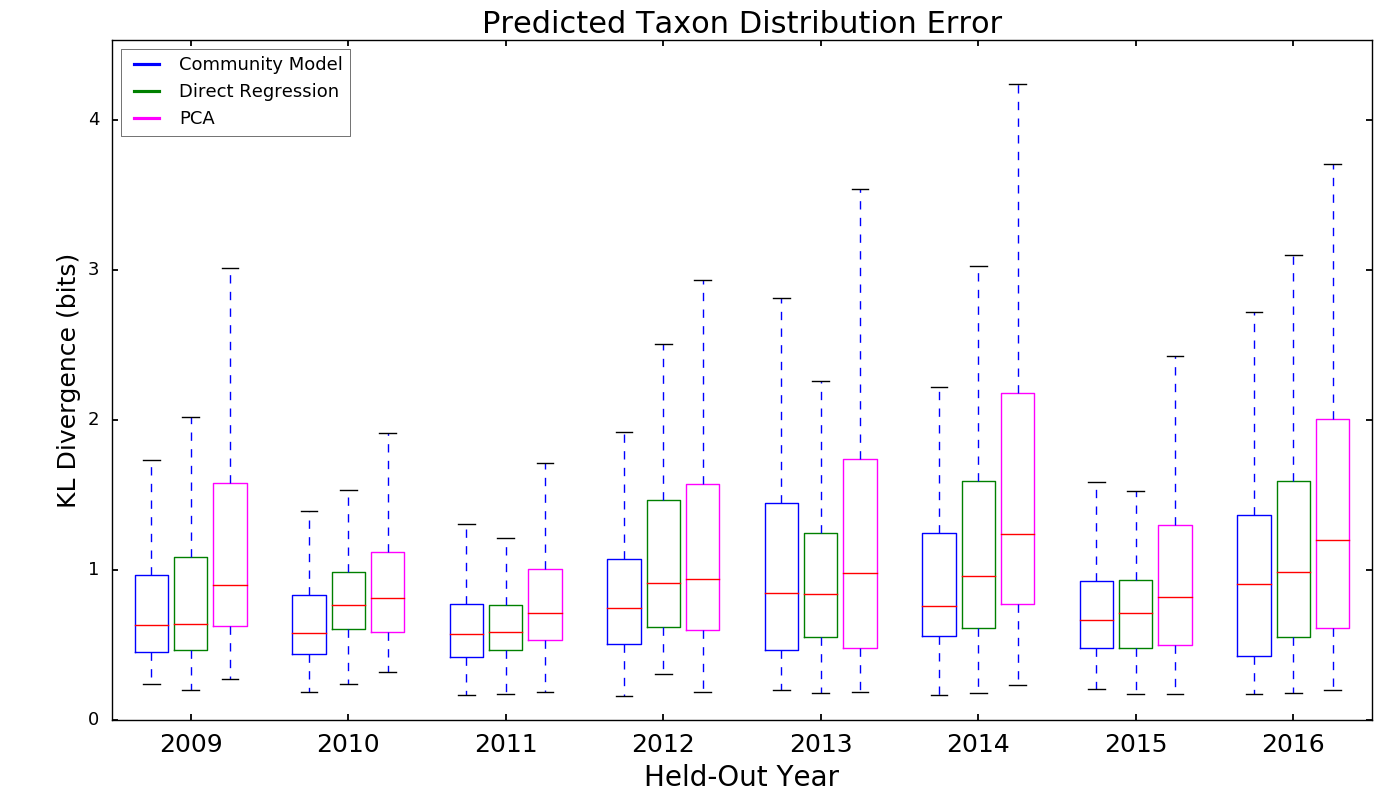
\includegraphics[width=0.8\linewidth]{figures/oceans/KLDivergenceBoxplot-C.png}
    \caption{Comparison of daily taxon distribution prediction divergences for each of the three regression methods and each of the years in the dataset. For each year, the other 6.5 years were used as training data. The community based regression method (ours, left) shows the lowest median KL-Divergence for all years.}
    \label{fig:plankton-mvco-kl-boxplot}
\end{figure}

We evaluated the resulting regression systems for all hyperparameter settings as well as the two baseline methods by comparing the predicted taxon distributions to the true distributions on each day in the dataset. Our error measure is the KL-Divergence between the predictions and the held-out distributons. We chose the community model with the lowest average KL-Divergence over all the days in the dataset, ultimately picking a model with 6 active communities. The predicted taxon distributions for this model are shown in Fig.~\ref{fig:plankton-mvco-word-est}.

Fig.~\ref{fig:plankton-mvco-kl-boxplot} shows the taxon distribution prediction errors for this community model and our two baseline models, broken out by year. The boxes represent the distribution of prediction errors for nearly 365 days in 2009 through 2015, and 172 days in 2016 (nearly 365 because of some small gaps in the taxon count data). Our community model (leftmost for each year) achieved the lowest median error on every year in the dataset. We found that by optimizing the hyperparameters for the regression task, we were able to choose an interpretable representation of the community structure. In contrast, PCA does not feature any prior for temporal smoothness. As a result although its prediction error is on average only a little less accurate than our model's, the sequences of predictions it makes are sometimes implausible, featuring taxon distributions which change much more rapidly than the observed data. We found that both baselines were extremely susceptible to noise in the environment data, on average performing better than expected, but occasionally making extremely poor predictions (Fig.~\ref{fig:plankton-mvco-timeseries}). With our model, the regression problem is of a lower dimensionality than for direct regression, and therefore less susceptible to overfitting. For this reason when both models are presented with the same small amount of training data, our model is more able to avoid large errors for new inputs unlike the training data.

\begin{figure}
    \centering
    \subfloat[]{
        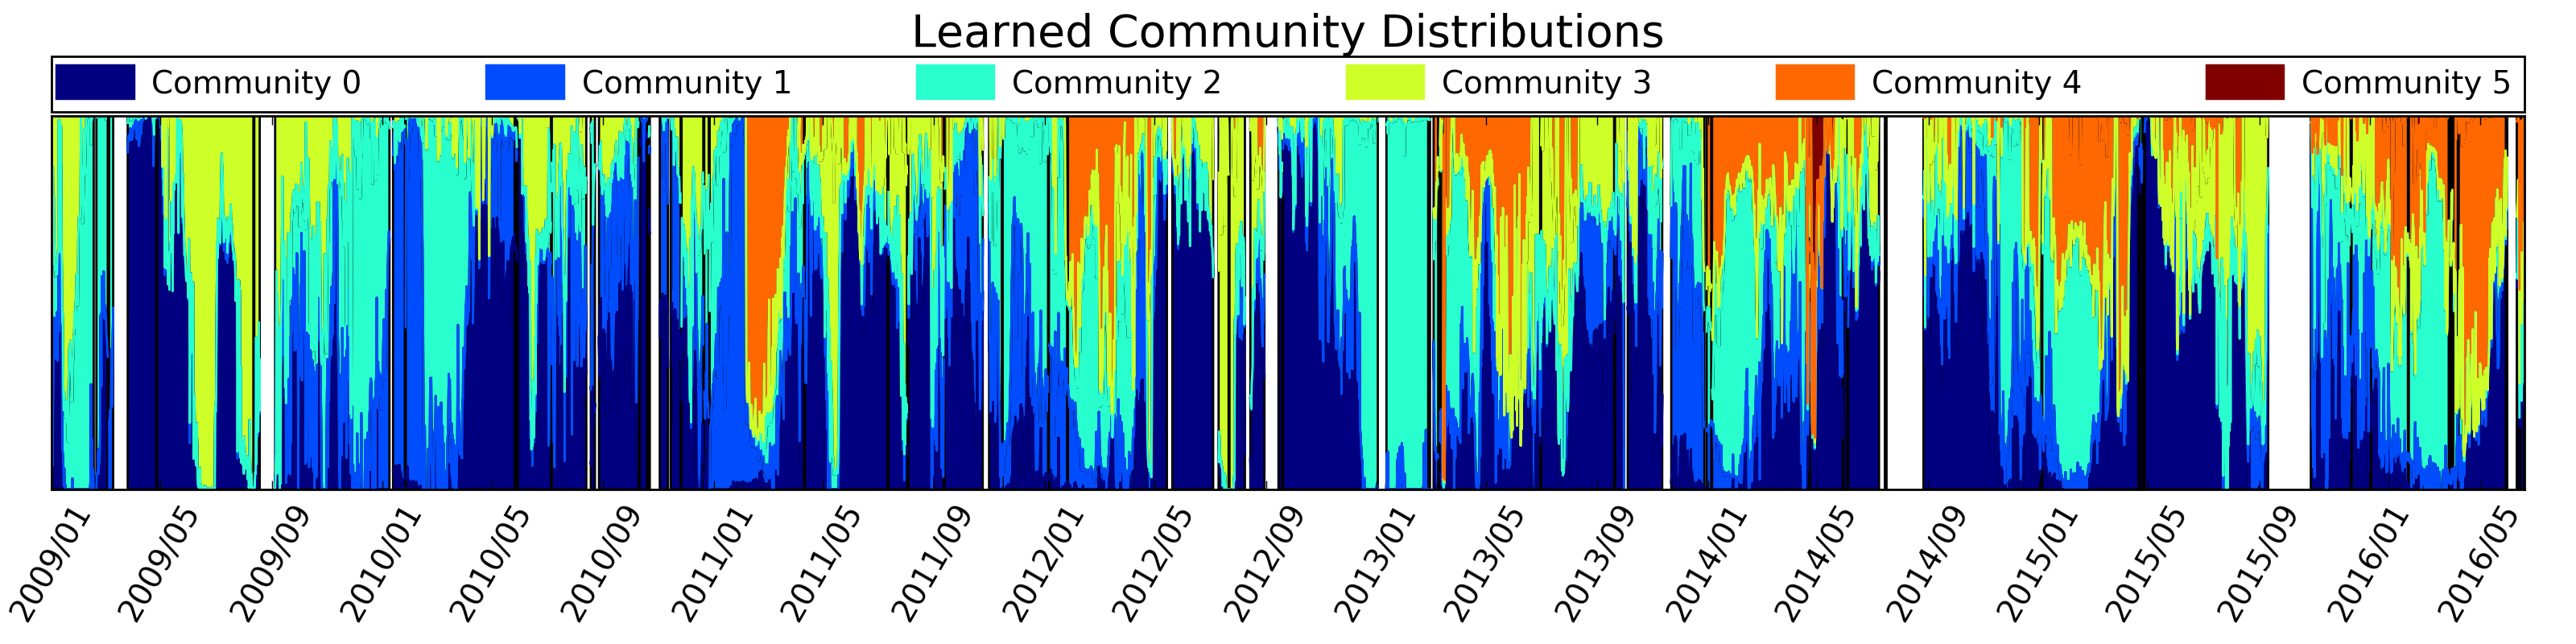
\includegraphics[width=\textwidth]{figures/oceans/theta_stacked.png}
        \label{fig:plankton-mvco-theta-stacked}
    }\\
    \subfloat[]{
        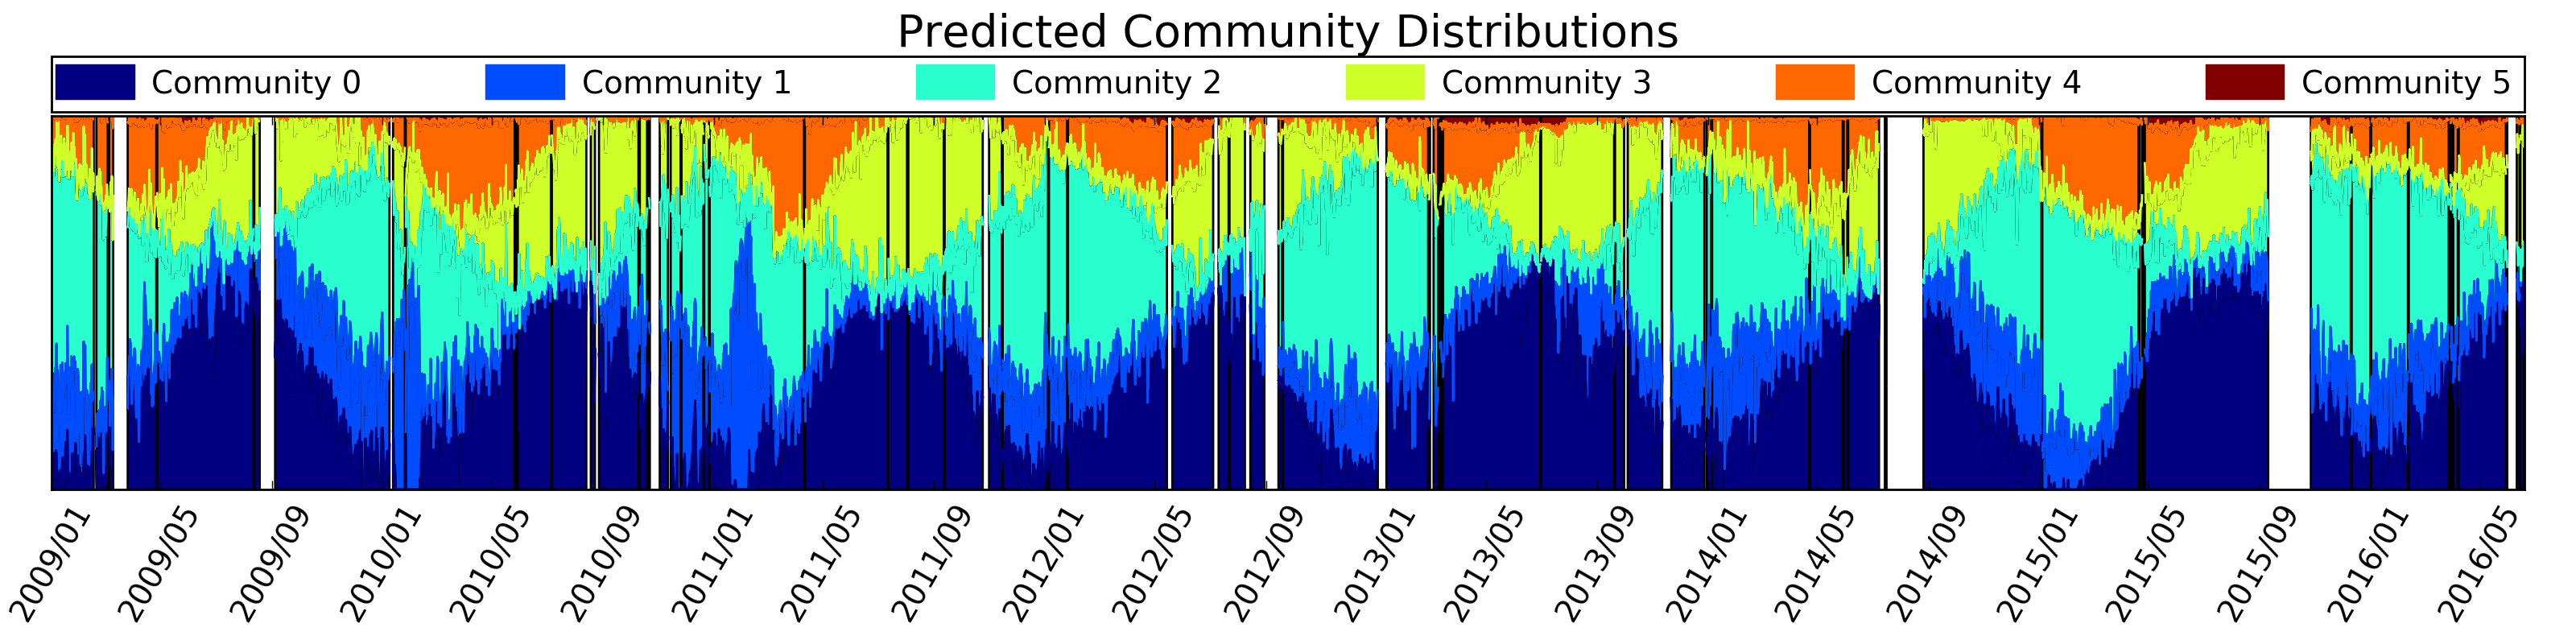
\includegraphics[width=\textwidth]{figures/oceans/theta_hat_stacked.png}
        \label{fig:plankton-mvco-theta-hat-stacked}
    }\\
    \subfloat[]{
        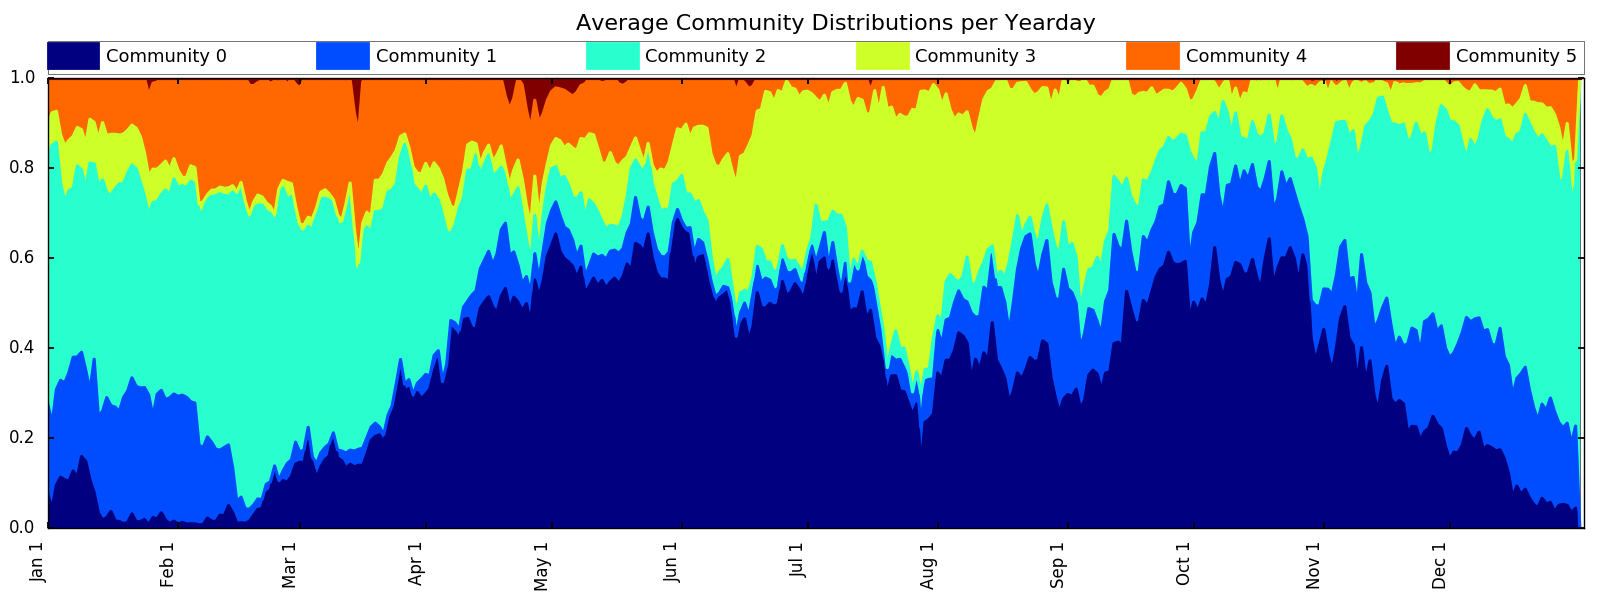
\includegraphics[width=\textwidth]{figures/oceans/theta_mod.png}
        \label{fig:plankton-mvco-theta-mod}
    }

    \caption{The learned and predicted community distributions. The horizontal axis represents time, and each community is represented by a color. The fraction of observations on a day belonging to a particular community are shown by the size of the colored area (totalling 1 for each day). Our model finds strong seasonal structure in the data without having such an assumption built-in.
    \protect\subref{fig:plankton-mvco-theta-stacked} Daily community distributions over 7.5 years for the best performing community model on the regression task.
    \protect\subref{fig:plankton-mvco-theta-hat-stacked} Daily community distributions predicted from environment data.
    \protect\subref{fig:plankton-mvco-theta-mod} Average community distribution for each day of the year over the entire dataset.
    }
    \label{fig:plankton-mvco-theta}
\end{figure}

An intriguing result of our community regression model is that nearly all of the magnitude in the weights of the learned regression parameters is either on the day of the year, the water temperature, or the number of plankton classified for a given day (Fig.~\ref{fig:plankton-mvco-weights}). 
From our regression matrix, we can see that each of the 5 communities has a seasonal niche with which most stongly predicts its presence. We found that the best performing community models showed strong seasonal structure, rather than relying on other variables. This is made evident by the average community distribution for each day of the year over the entire dataset before regression (Fig.~\ref{fig:plankton-mvco-theta-mod}). Note that there are many possible community decompositions, and although our model makes weak assumptions about the temporal smoothness of the communities, it does not have any prior knowledge of the seasonal nature of the data. By performing hyperparameter optimization over the downstream regression task, we were able to select a model with just the right level of sparsity and temporal smoothness to emphasize this seasonal aspect and describe the data in an interpretable way.

\begin{figure}
	\centering
	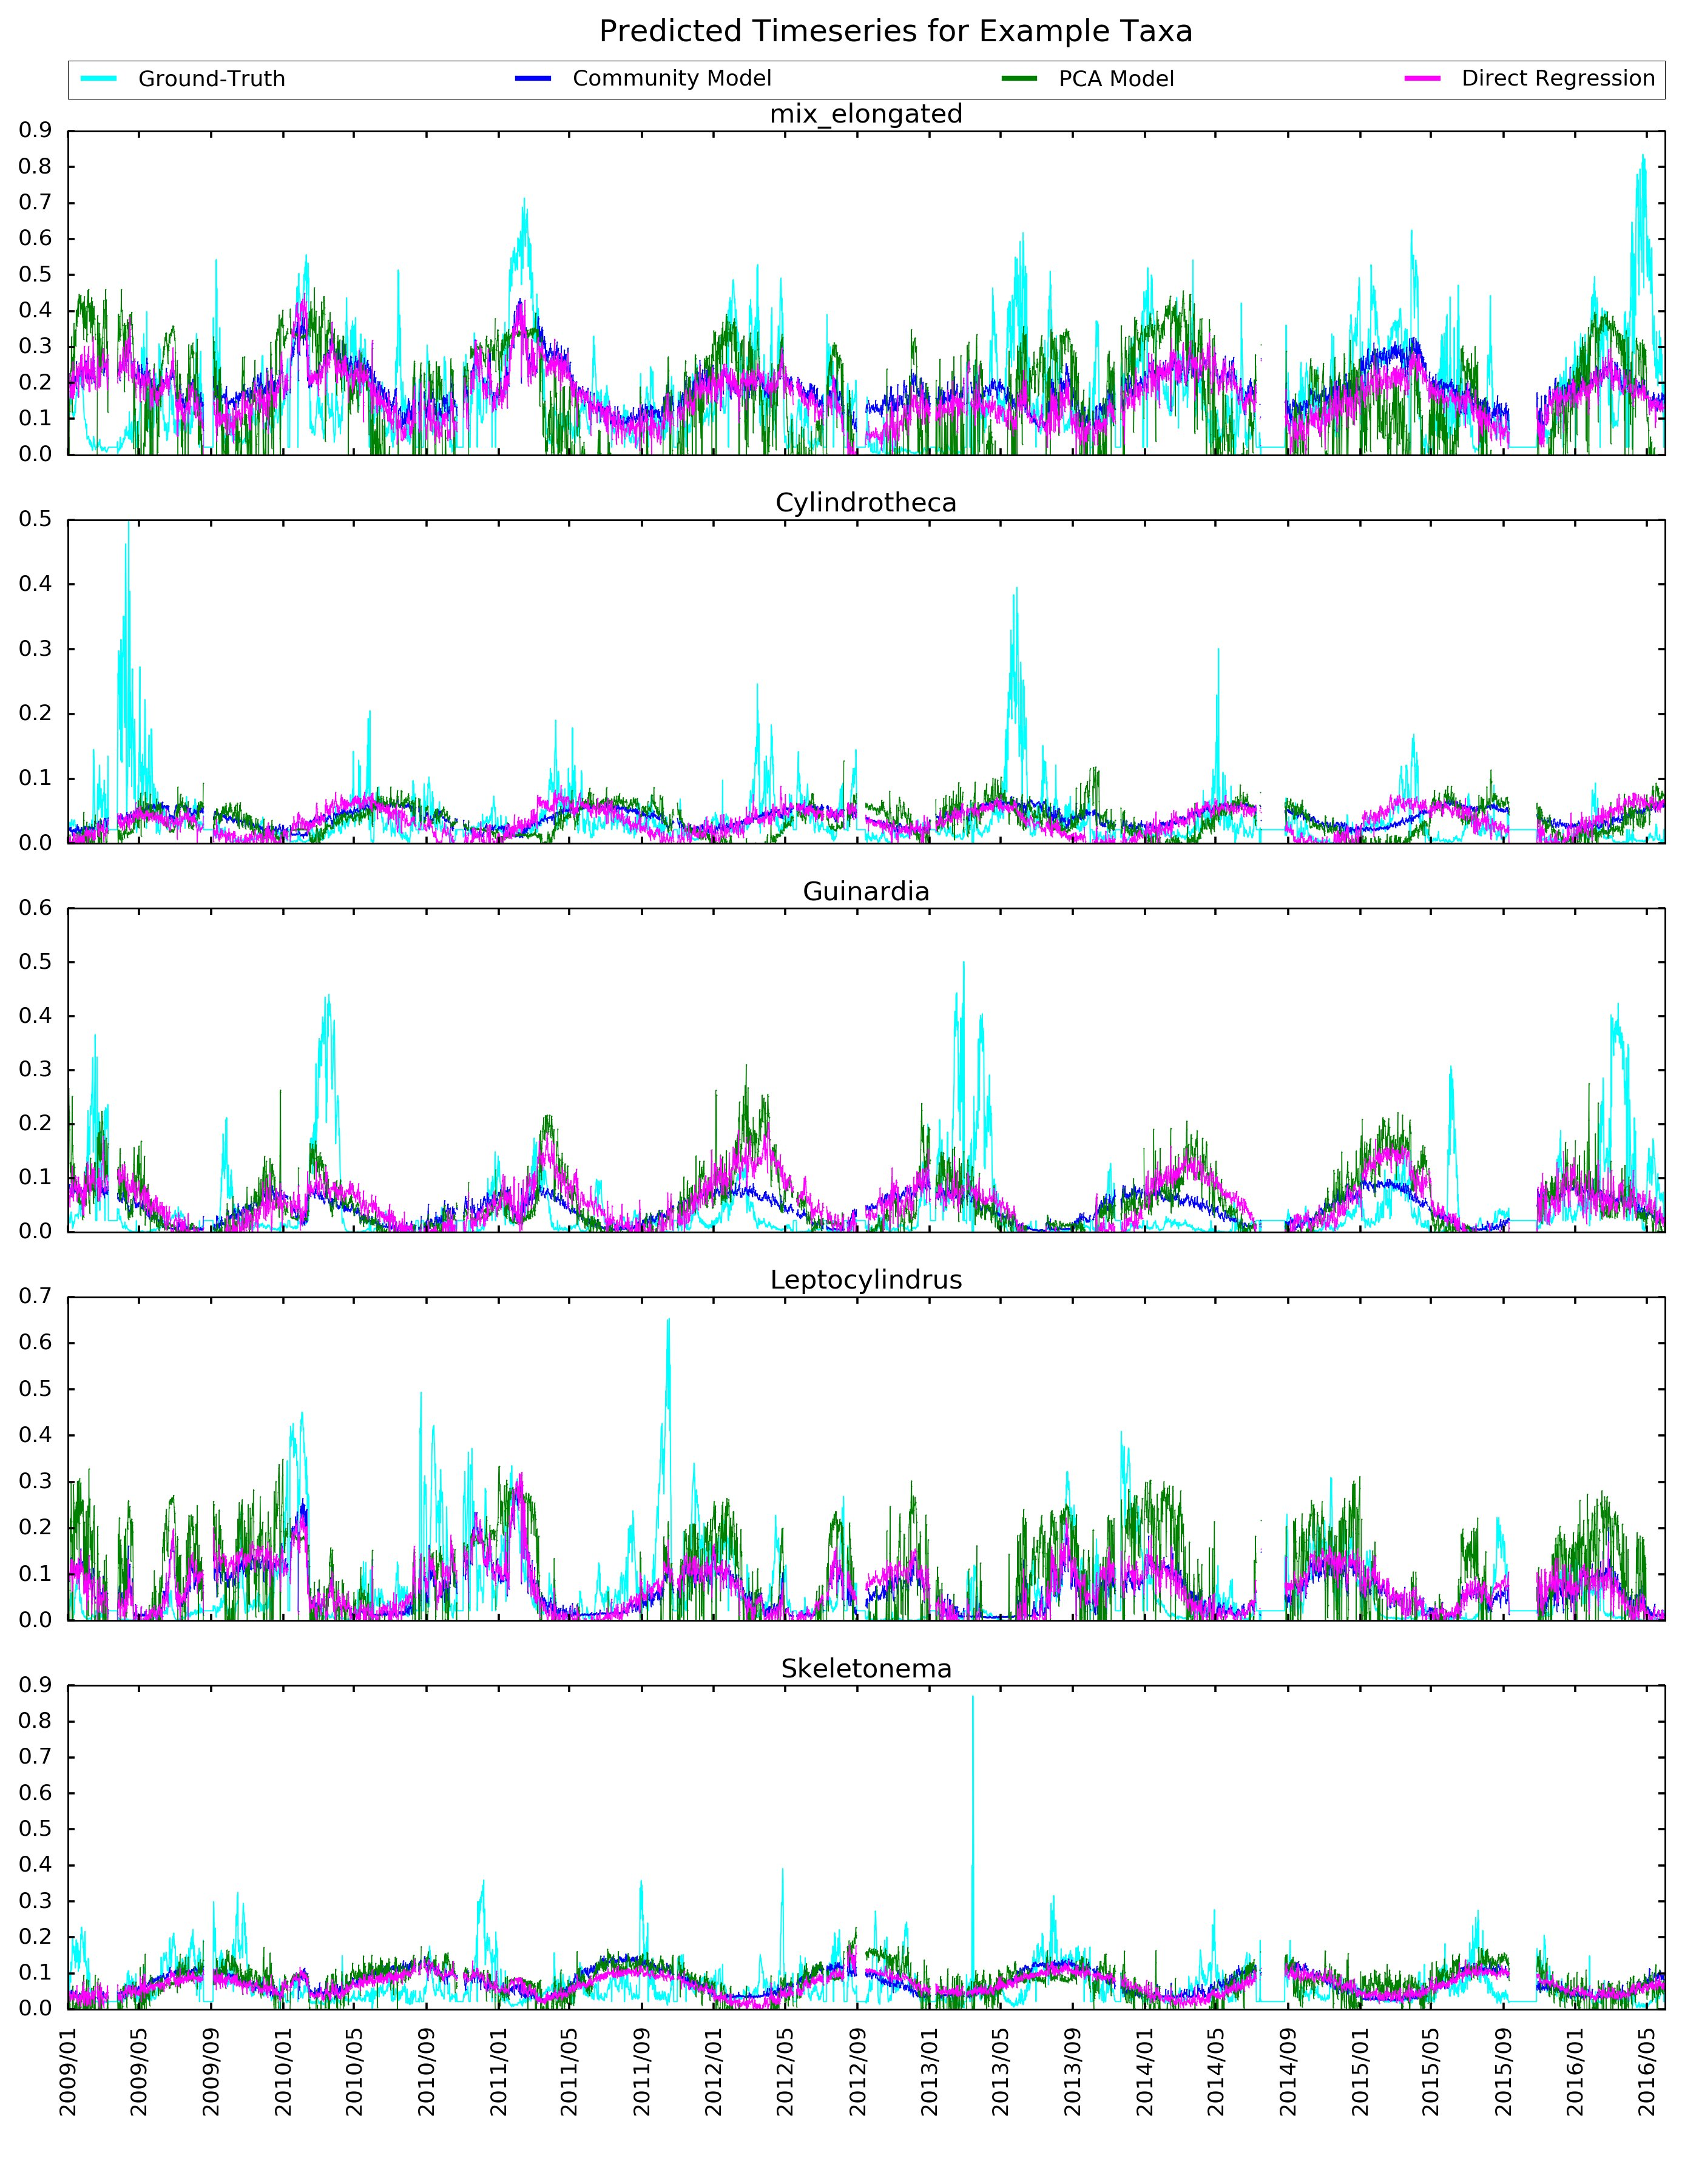
\includegraphics[width=0.95\textwidth]{figures/oceans/timeseries.jpg}
	\caption{Timeseries representation of individual probability of observing 5 common taxa on each day in the dataset. Note that the community model's predictions are less susceptible to noise that the other two strategies.}
	\label{fig:plankton-mvco-timeseries}
\end{figure}

Another outcome of our experiment is the communities themselves learned by our model (Fig.~\ref{fig:plankton-mvco-phi}). We found that across different hyperparameter choices, the top few most active communities were relatively similar to those presented here. Some associations based on our model have ready explanations. For instance community 1 is dominated by the taxa ``mix\_elongated'', representing miscellaneous centric diatiom chains, and ``leptocylindrus'', which both exhibit elongated morphologies and easily confuse the IFCB's vision-based classification system. As a more exciting example, communities 2 and 4 are the only communities with significant probability of observing the taxon ``Guinardia'', and are predicted by warm water temperatures, while \emph{Guinardia delicatula} populations have been noted to be negatively associated with parasites that do not survive during cold winters \citep{peacock2014parasitic}.

\begin{figure}
    \begin{center}
        \subfloat[]{
            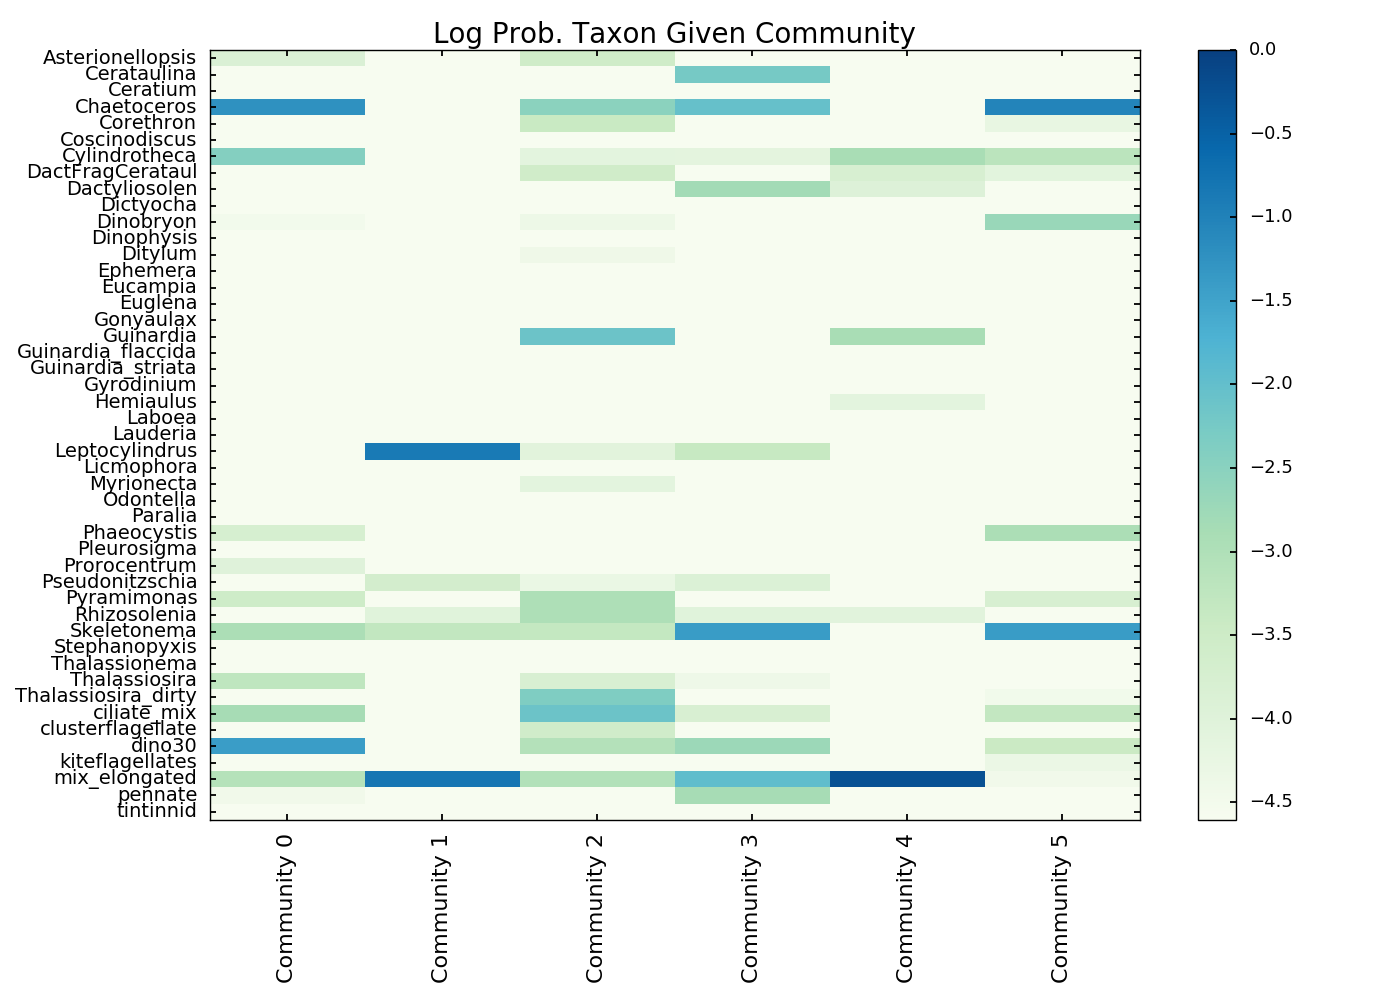
\includegraphics[width=0.49\columnwidth]{figures/oceans/LogPhi.png}
            \label{fig:plankton-mvco-phi}
        }%
        \subfloat[]{
            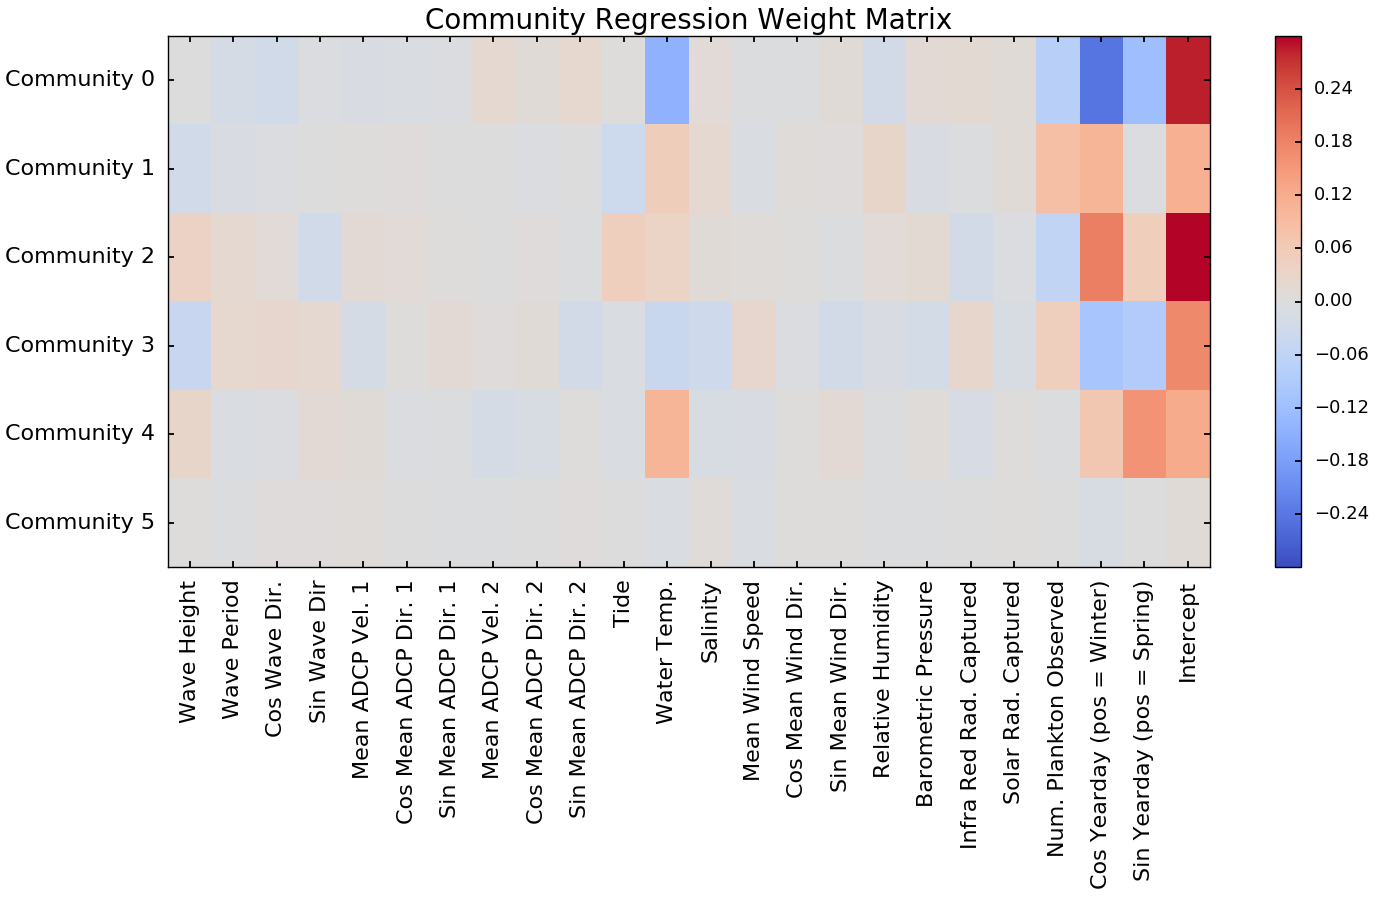
\includegraphics[width=0.49\columnwidth]{figures/oceans/weights.png}
            \label{fig:plankton-mvco-weights}
        }
    \end{center}

    \caption{
        \protect\subref{fig:plankton-mvco-phi} Log-probability of each taxon for each community.
        \protect\subref{fig:plankton-mvco-weights} Linear regression weight matrix for top-performing community model.
    }
    \label{fig:plankton-mvco-supplemental}
\end{figure}

Our community model takes a complex, high-dimensional population dataset, and offers immediate questions to pursue related to the ecology of specific taxa near MVCO. For instance, in Fig.~\ref{fig:plankton-mvco-theta-stacked} we see that community 4 begins to appear a little earlier each year from 2011, at first appearing only in the spring, and by 2015 persisting throughout the Winter. If we were to only look at the timeseries for the individual taxa, ``mix\_elongated'', ``Guinardia'', and ``Cylindrotheca'' which dominate community 4, this pattern is not obvious at all (See Ground-Truth, Fig.~\ref{fig:plankton-mvco-timeseries}). However, our model highlights that these taxa often co-occur, and that the pattern of co-occurrence shifts over the years.

\section{Predicting presence of missing phytoplankton by their associates} \label{sec:plankton-spatial-search}
In our second study of IFCB plankton data, we ground our community model by its ability to predict the presence of an artificially held-out plankton taxon from the others, rather than predicting the full distribution from auxillary data \citep{Kalmbach2017a}. Further, in this application we explore spatial phytoplankton classification data, demonstrating our model's ability to capture both the temporal and spatial smoothness aspects of community structure. This work is motivated by a scenario where a plankton ecologist is searching for a particular plankton taxon. If the ecologist deploys IFCB on a ship and periodically collects samples, but never observes the taxon of interest, she requires further information to decide whether to move on or keep collecting samples in the same location. Because IFCB samples are a small volume of water, yet ecologists would like to describe large volumes of ocean that have complex ecosystems, it is very likely that samples will sometimes be deficient in taxa that are, in fact, found near the sample location. Therefore, we propose to model the associations between taxa in such a way that if we disregard the target taxon we can still estimate the community mixture for a location accurately, and consequently predict the presence or absence of the target from its known assocaites.

We would like to estimate the probability of observing a falsely-missing target taxon $v^\star$, based on the observed distribution of the $V-1$ other taxa.
We assume that the taxon is not systematically missing, in other words that we can collect a training set at some other locations comprised of all $V$ taxa.
Then given this training set, we learn the topic assignments and MLE priors $\hat{\Theta}$ and $\hat{\Phi}$. At test-time we disregard the target taxon, assuming it is falsely-missing. To address this we consider the topics excluding $v^\star$ as the maximum likelihood of the Dirichlet over the other $V-1$ taxa. In other words, at test time we use topics which ignore the missing taxon:
\begin{equation}
P(w = v | z = k, \boldsymbol{w}) \approx \hat{\Phi}_k^{-v^\star} \triangleq \frac{N^{w_i}_k + \beta}{\sum_{u \neq v^\star} N^u_k + \beta},
\end{equation}

Next, we obtain topic assignments $\boldsymbol{z_{- v^\star}}$ by substituting $\hat{\Phi}_k^{- v^\star}$ for $\Phi$ in the predictive distribution Eqn.~\ref{eqn:posterior}. In the iterative process of sampling topic assignments, we fix $\hat{\Phi}_k^{-v^\star}$, and only update topic assignments for new observations based using the `target defficient' topic assignment counts. These define the approximate MLE topic priors $\check{\Theta}_{g(x)}$. Finally, we estimate the proportion of the data which would have been made of the target class using the original MLE topic matrix
\begin{equation}
P(w_x = v^\star) = \sum_{k=0}^K \check{\Theta}_{g(x),k} \hat{\Phi}_{k,v^\star}
\end{equation}

\subsection{US Atlantic coast hotspot prediction experiment}

We demonstrate this approach with IFCB classification results from NOAA's Fall 2014 EcoMon Survey aboard the Research Vessel Pisces (Cruise PC 14-05). The IFCB was configured to automatically sample from underway flowing surface seawater during the period 4-19 November 2014. The classification system generated over 140,000 individual phytoplankton observations from these water samples. Classification results comprise a dataset with 47 taxa at 852 locations spanning the US Atlantic coast from North Carolina to Maine (See Fig.~\ref{fig:plankton-pisces-summary-in}).

\begin{figure}
	\centering
	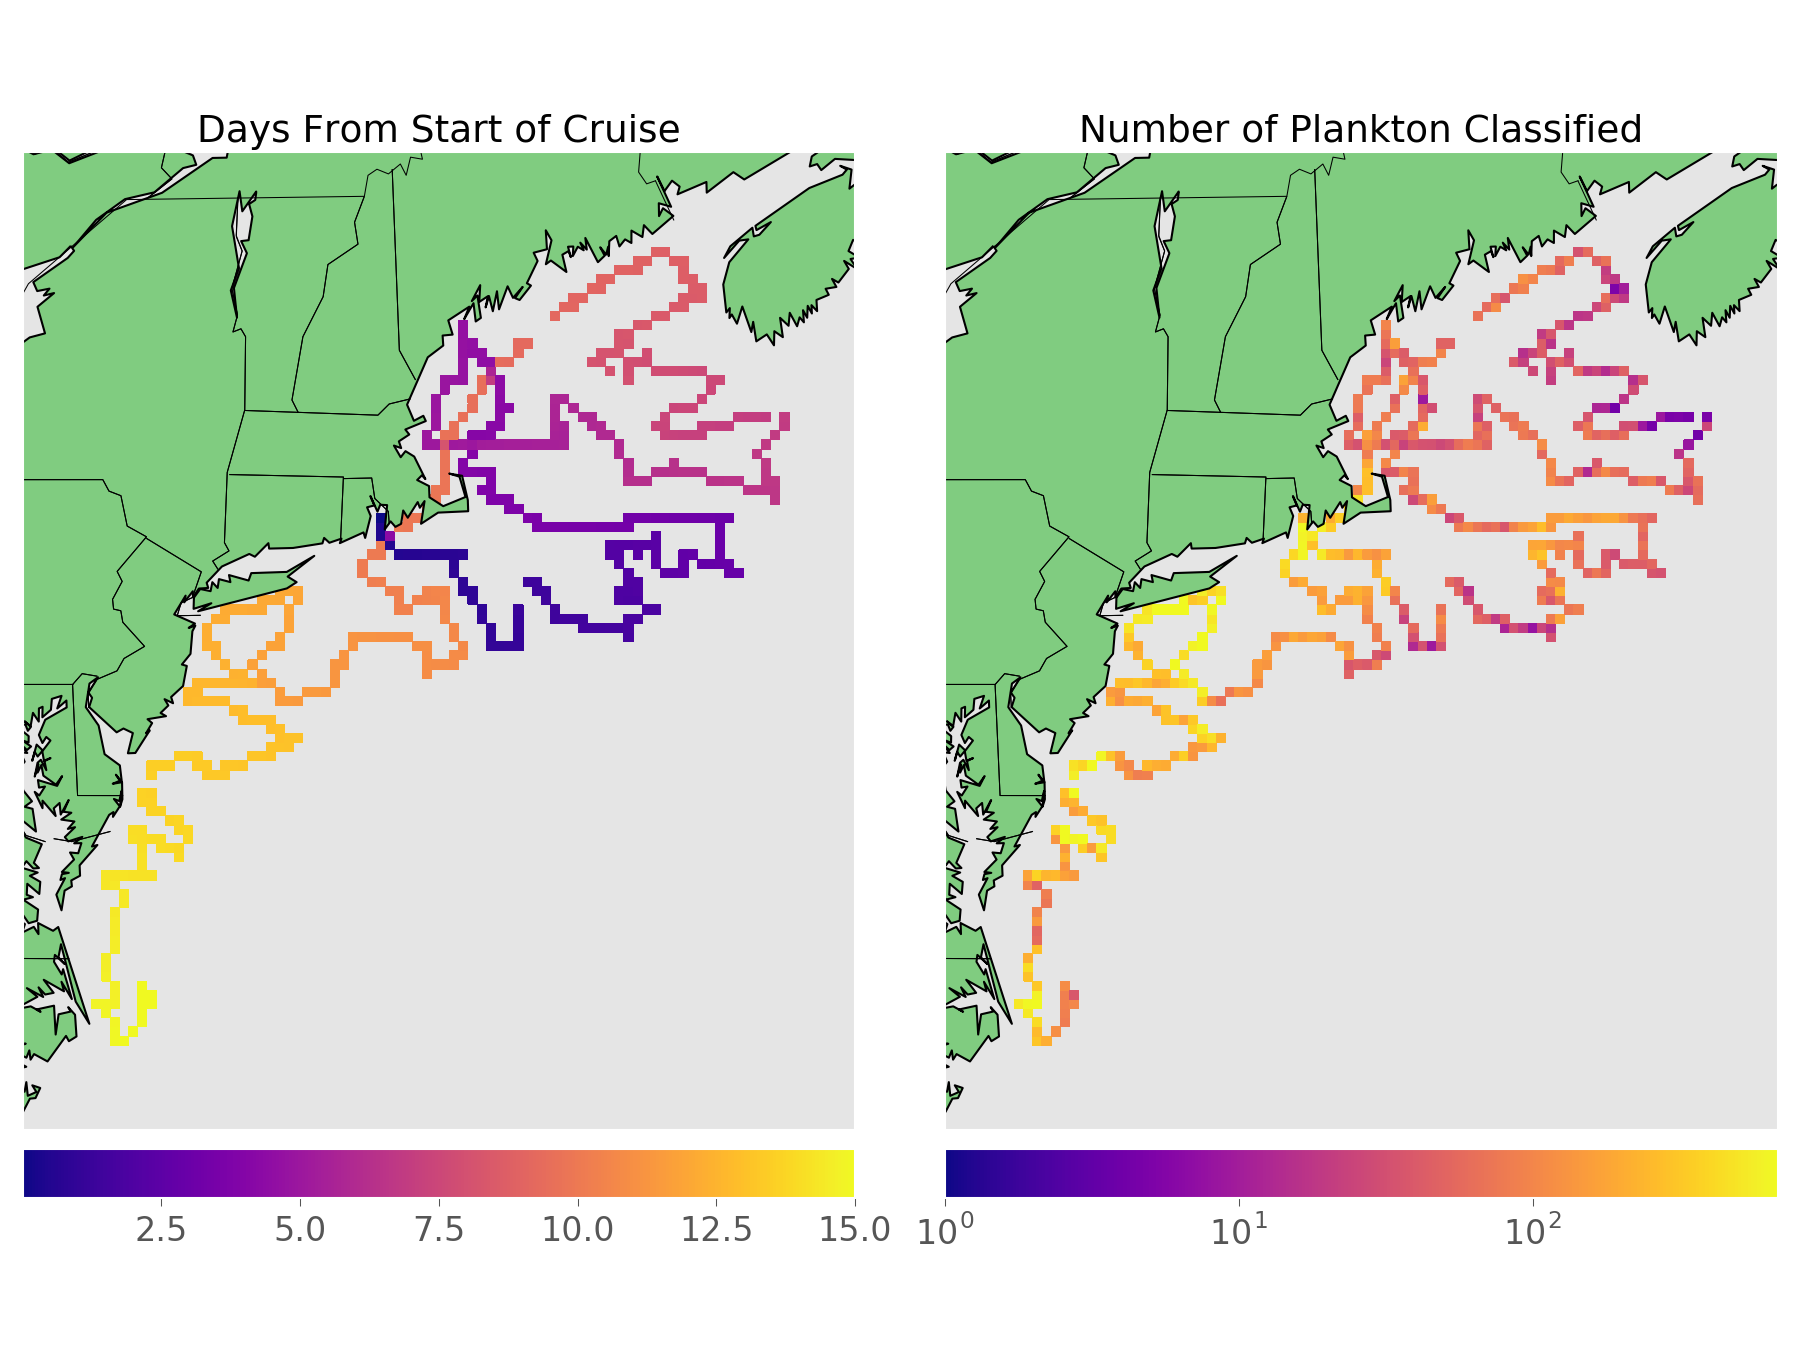
\includegraphics[width=0.75\textwidth]{figures/icra_plankton/n_plankton.png}
	\caption{Summary of data recorded during the Pisces 14-05 cruise. Left, color shows progress in time. Right, color shows the number of plankton observed at each sample location.}
	\label{fig:plankton-pisces-summary-in}
\end{figure}

We divide the sample locations into equal-sized parts, representing the training and test phases of the simulated mission. The counts of all 47 taxa were kept in the training set and used to learn the topic model. For the test set, we held out each of the 8 most-frequently observed phytoplankton taxa one at a time. We define the hotspots of
a taxon to be the top 50 sample locations in the test data, where the relative abundance of the taxon to all other taxa was highest. The 8 tested taxa make up just over 81\% of all the observations in the dataset. The most common taxa are miscellaneous centric diatom chains (``mix\_elongated''), mixed species of pennate diatoms, \emph{Thalassiosira} spp., \emph{Guinardia delicatula, Guinardia striata, Dictyocha} spp., \emph{Ephemera} spp., and \emph{Phaeocystis} spp. While our method accounts for the sparsity of taxon distributions, this dataset also features sparsity in terms of the locations of observations. To address this separate issue, we resort to a 2D spatial median filter. Finally, we apply a threshold to identify the hotspot locations.

We compared our method to an exhaustive search strategy and a k-means search strategy. For each sample in the test set, exhaustive search estimates the probability of observing $v^\star$ by looking up the sample in the training set with the most similar distribution to the observed data. This represents the strategy which makes the most use of all the data available for every test sample, at the cost of a linear computational complexity in the number of sample locations in the dataset. In the k-means strategy, we fix a constant test-time complexity by reducing the search space to the $K$ centroids returned by a standard k-means clustering implementation. These centroids are defined such that if each class distribution in the training set were replaced by the nearest of the $K$ centroids, the sum of squared error is approximately minimized, however it does not take into account the sparsity or spatial smoothness of the underlying distributions.

We carried out experiments for two different train/test regimes. First, we used every second sample location for training (see Fig.~\ref{fig:plankton-pisces-maps-8}, column 1). This regime simulates a mission where the classifier frequently fails to identify examples of a class, for instance because its classifier was poorly tuned. Because nearby sample locations tend to have similar distributions, this regime tests the ability of a model to interpolate over small distances. Second, we used the first half of the sample locations as training (Fig.~\ref{fig:plankton-pisces-maps-1}, column 1), and the second half for testing. This latter case simulates a mission where the capabilities of the classifier have changed from the first half to the second half. It tests the ability of a model to predict in a new location that is not likely to have any spatially linked correlation with the training data.

\begin{figure}
    \centering
    \resizebox{0.9\textwidth}{!}{%
        \begin{tabular}{c}
        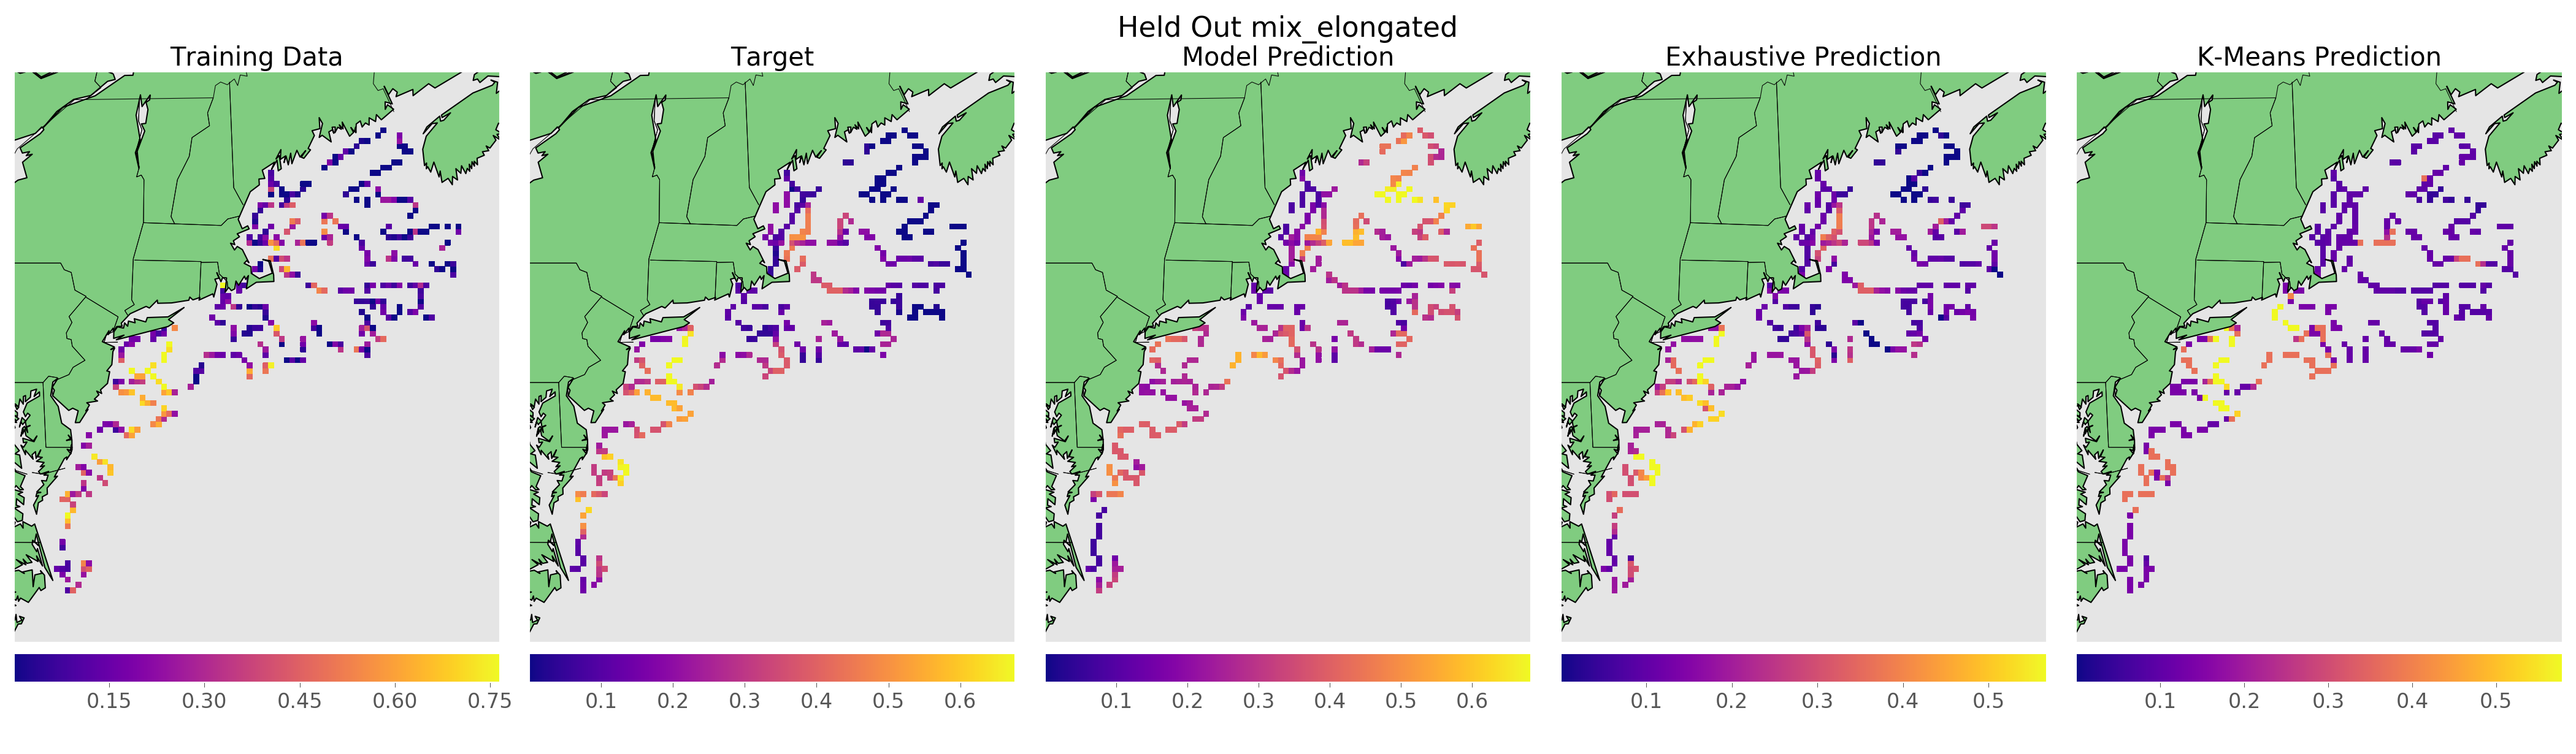
\includegraphics{figures/icra_plankton/maps_mix_elongated_8} \\
        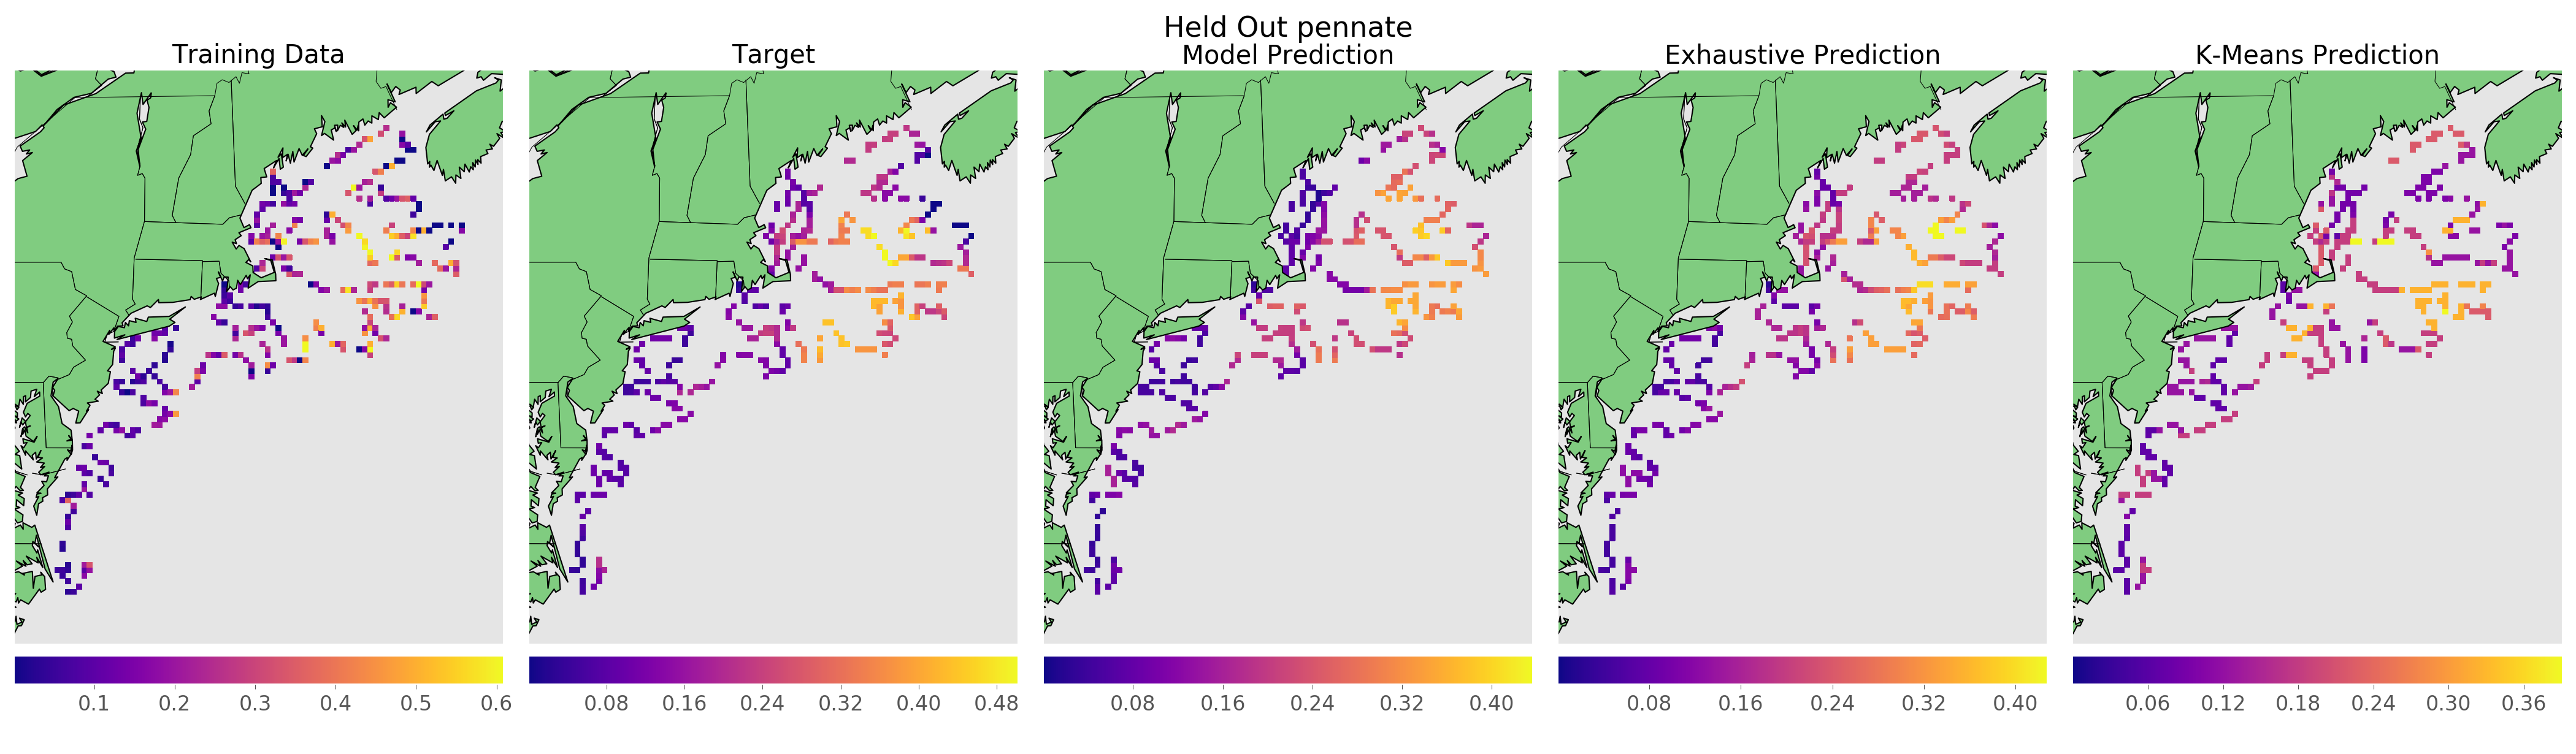
\includegraphics{figures/icra_plankton/maps_pennate_8}\\
        +
        %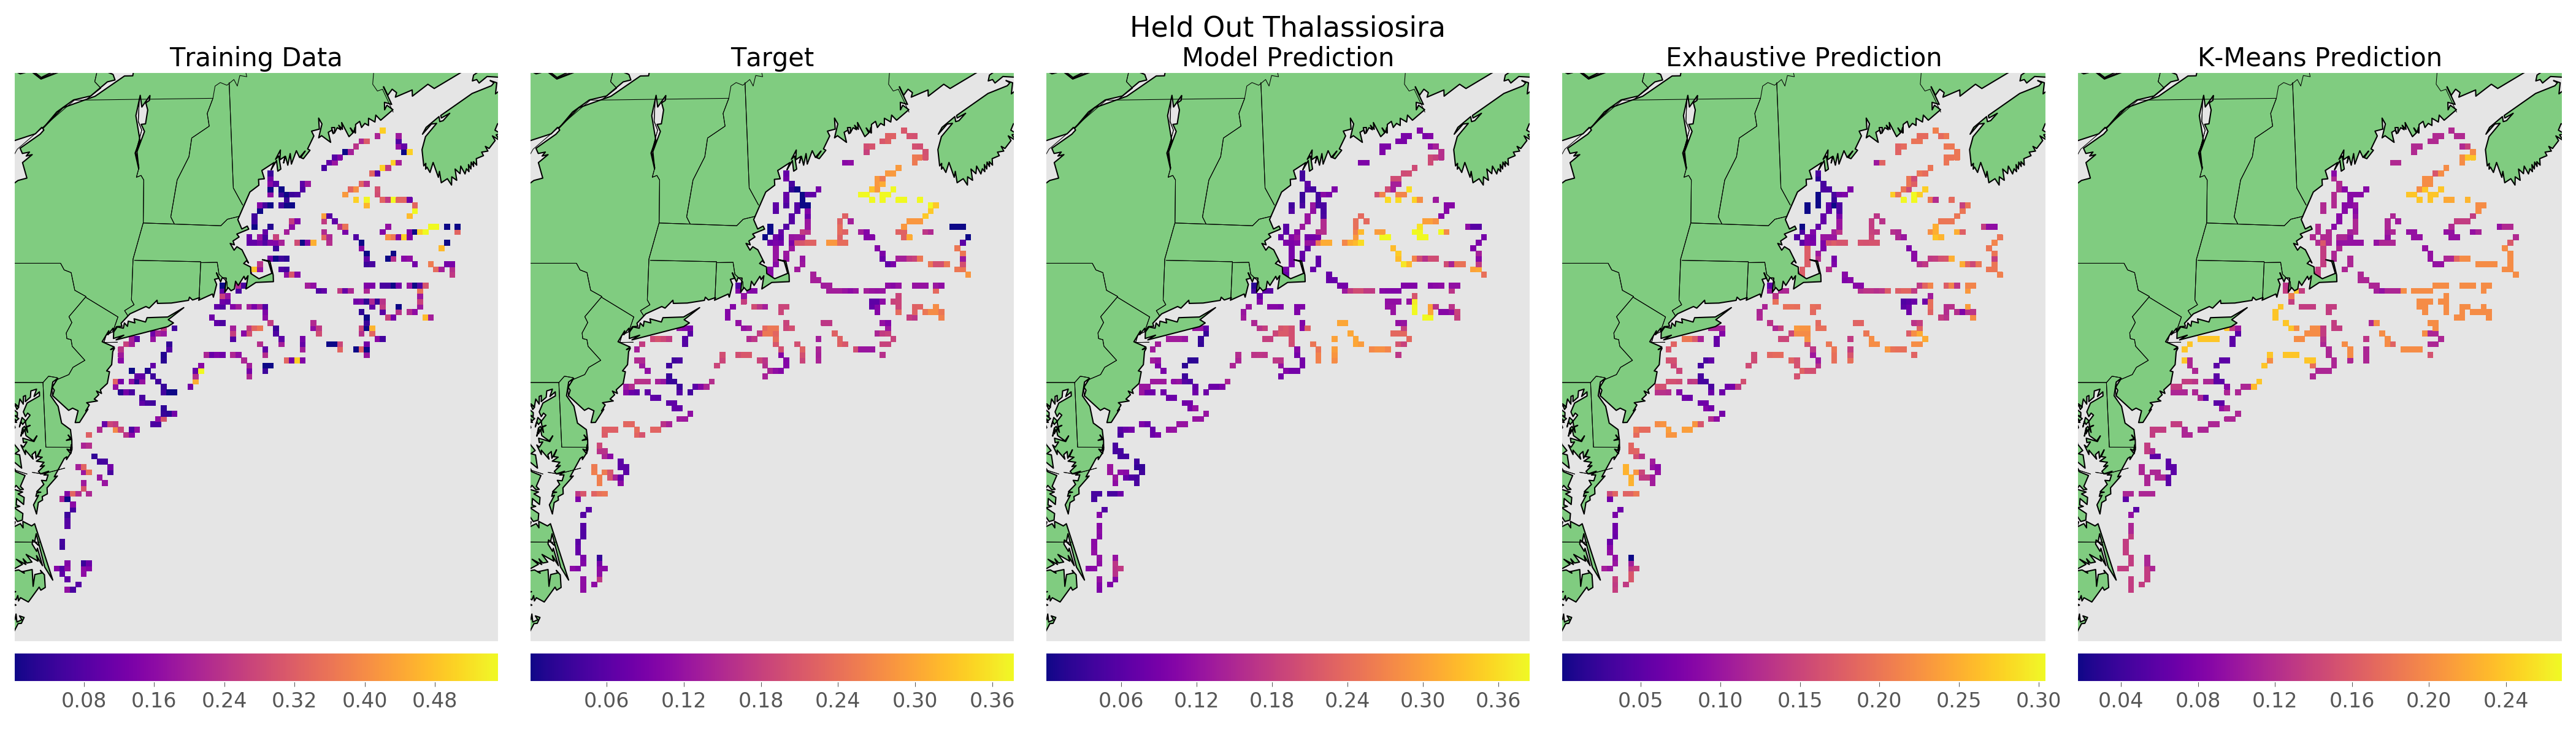
\includegraphics{figures/icra_plankton/maps_Thalassiosira_8}\\
        % 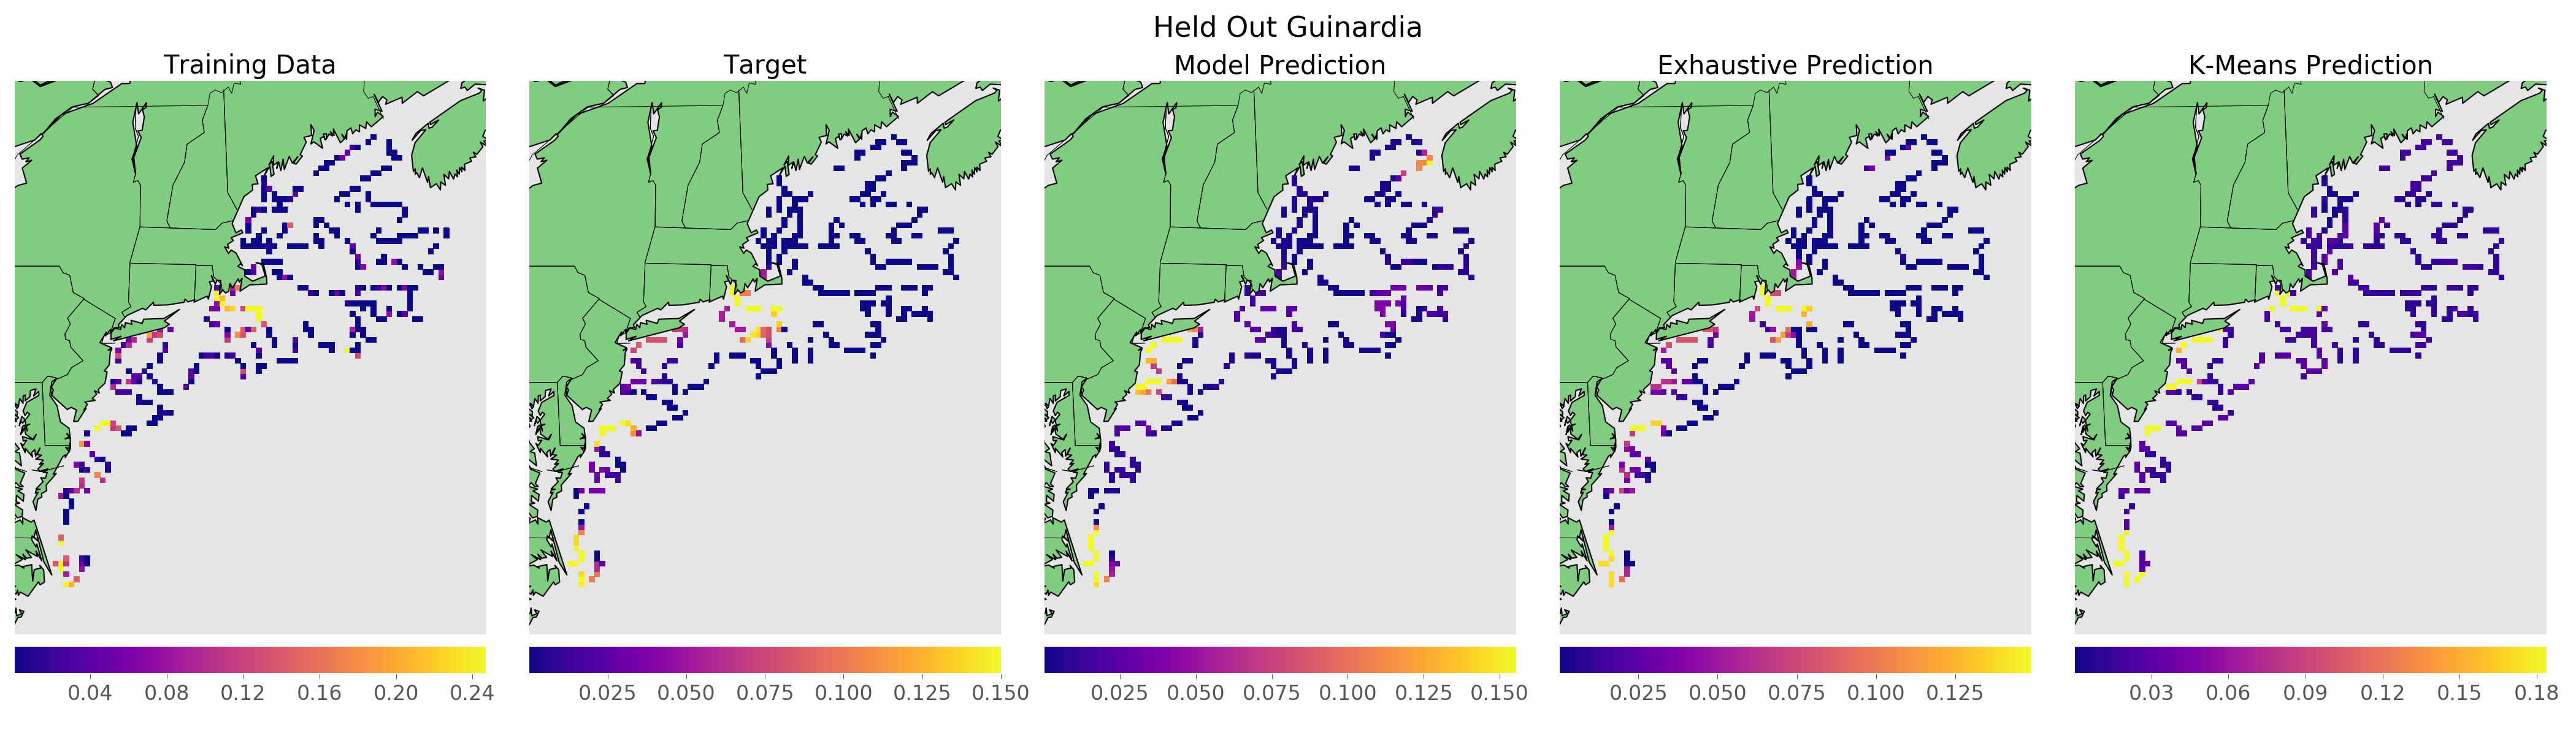
\includegraphics{figures/icra_plankton/maps_Guinardia_8}\\
        % 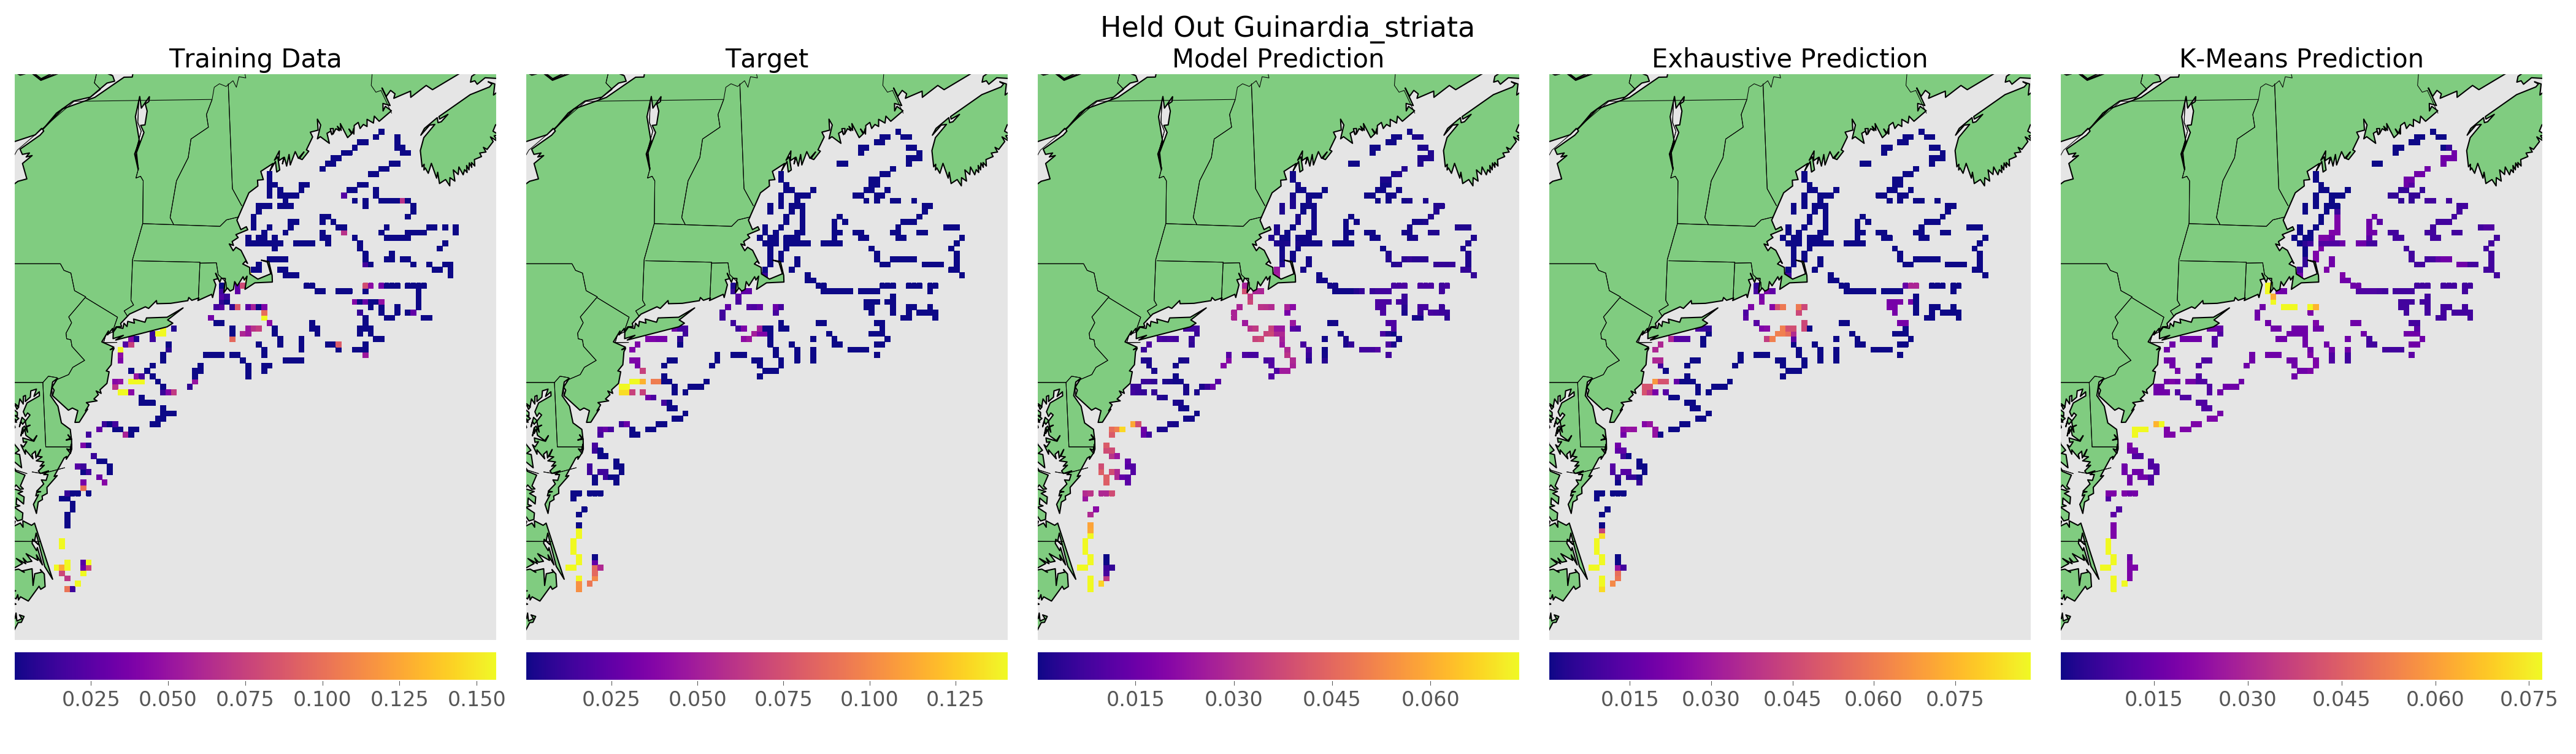
\includegraphics{figures/icra_plankton/maps_Guinardia_striata_8}\\
        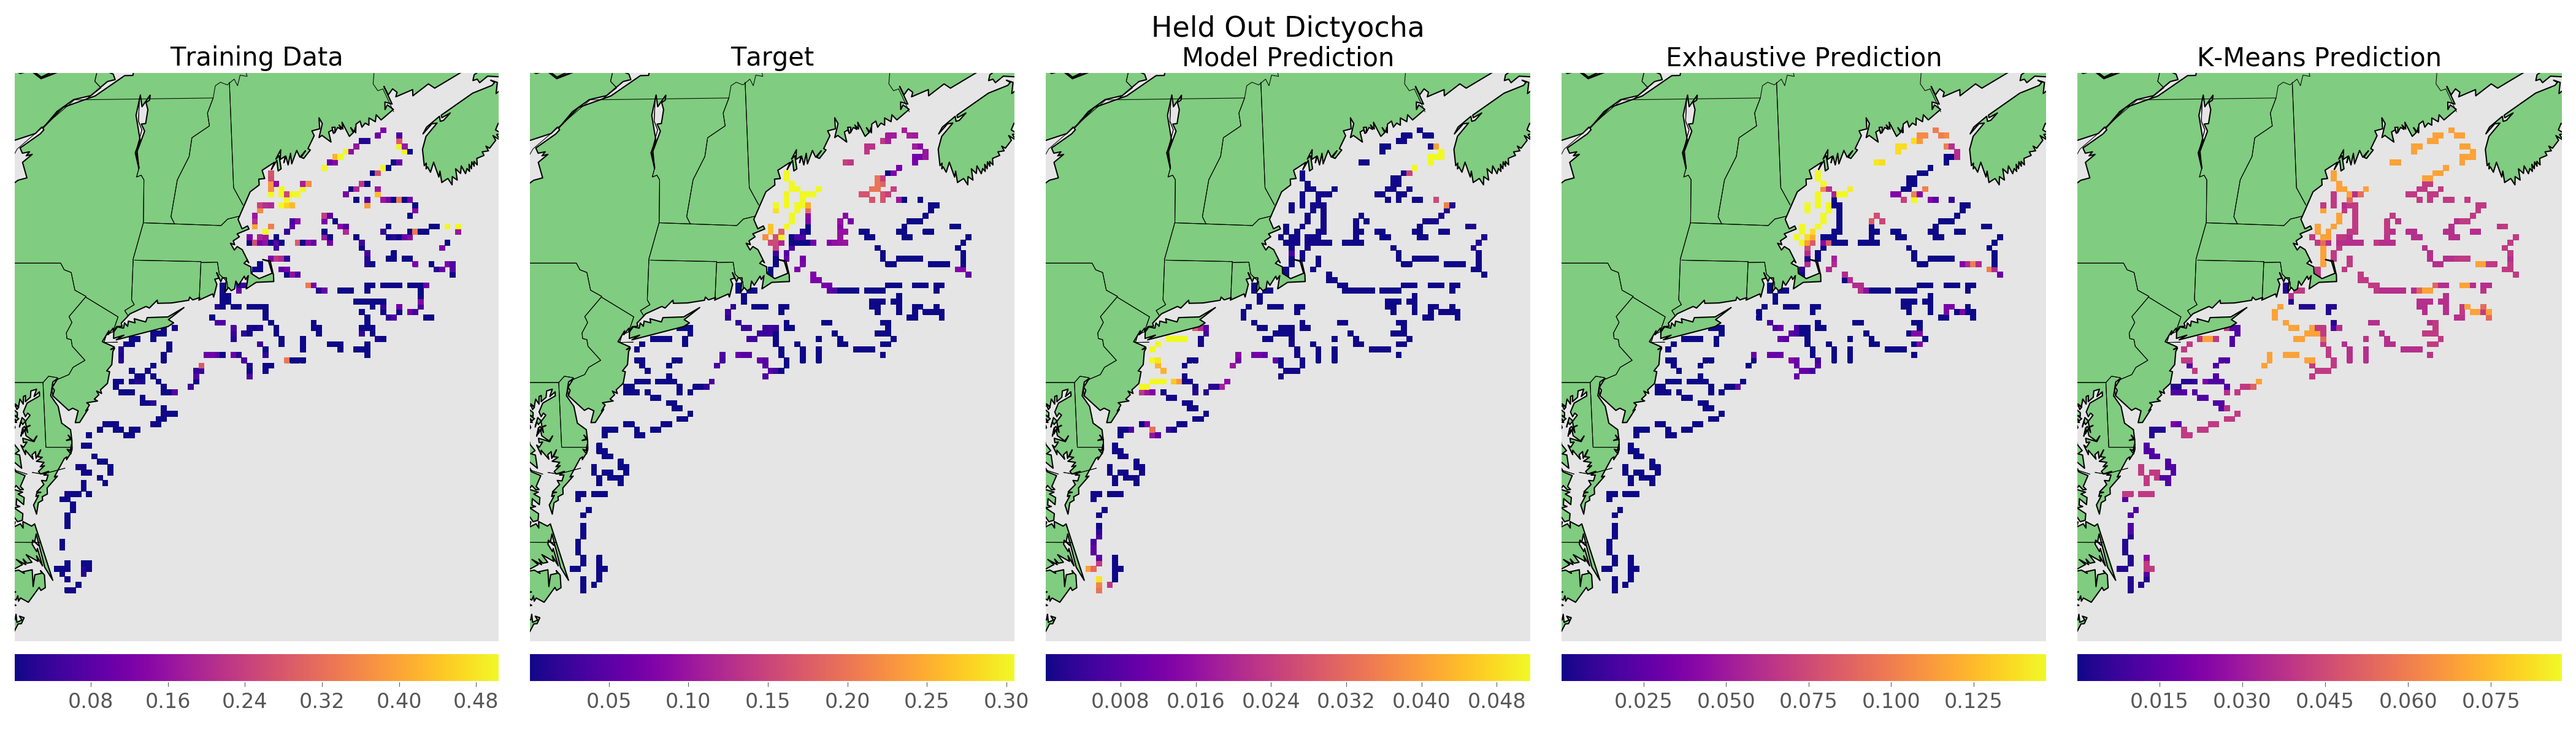
\includegraphics{figures/icra_plankton/maps_Dictyocha_8}\\
        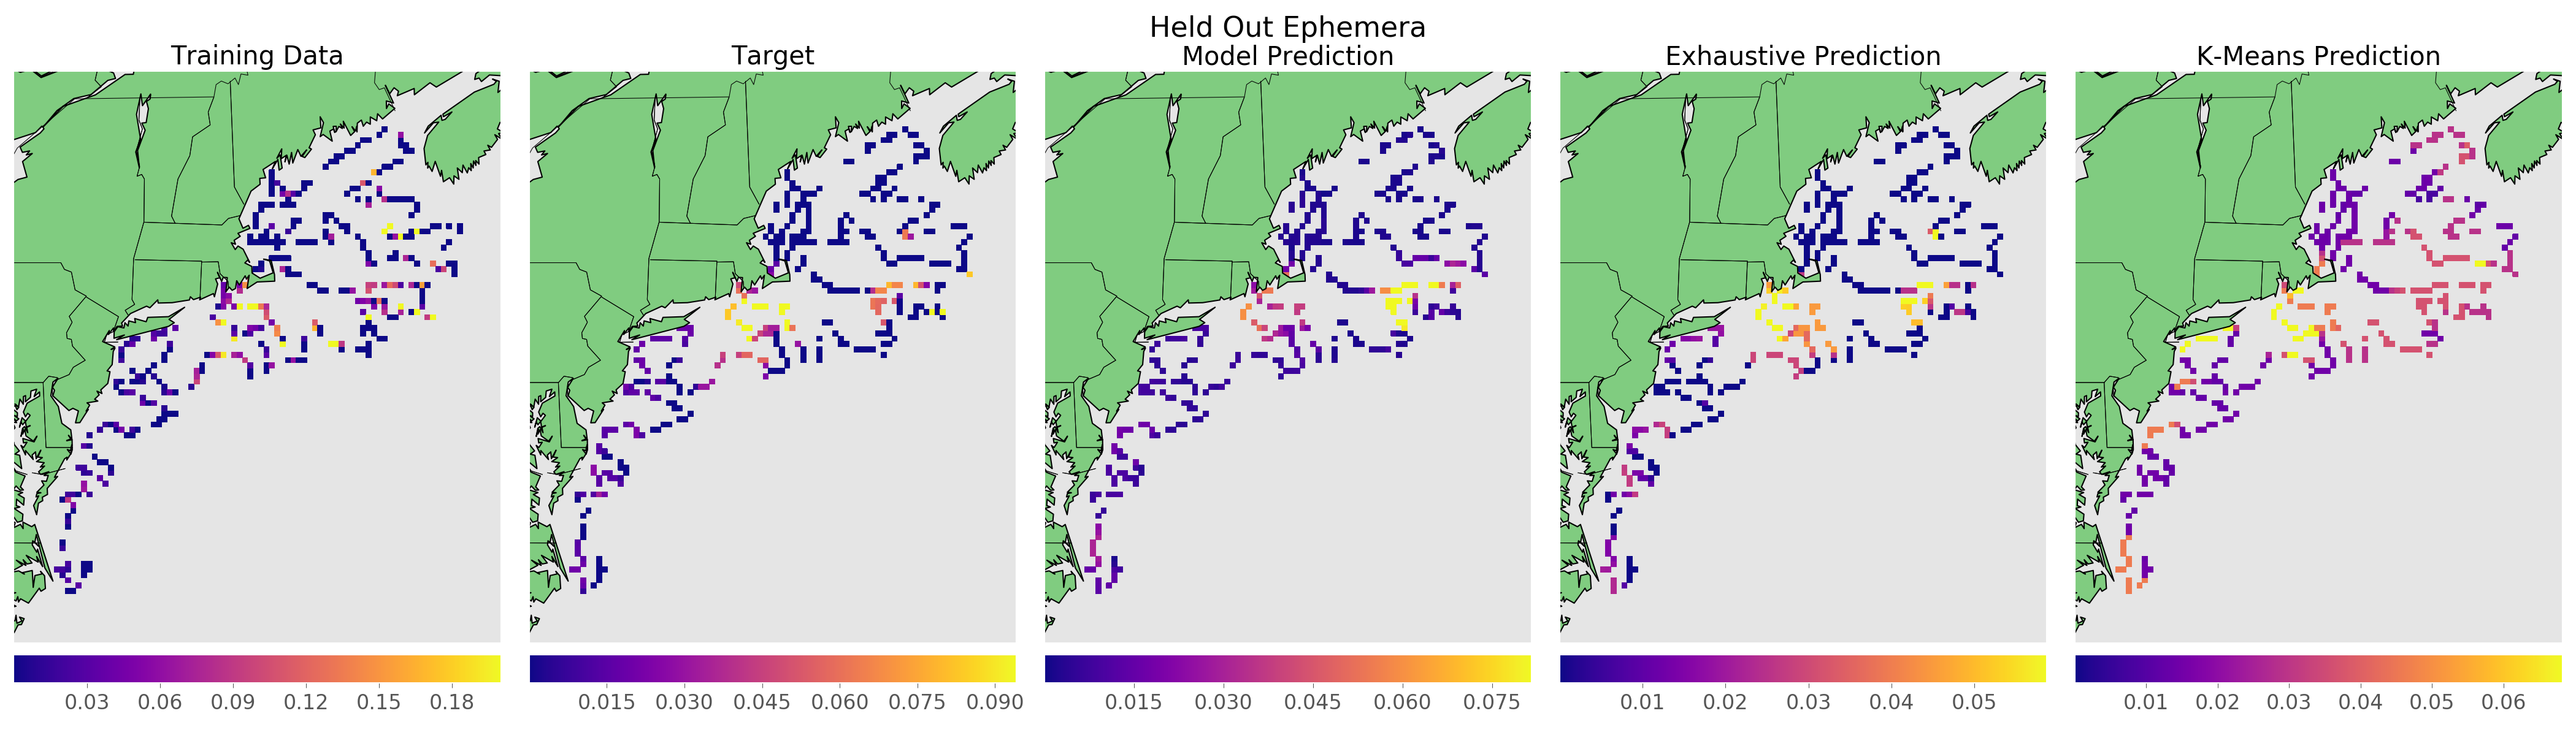
\includegraphics{figures/icra_plankton/maps_Ephemera_8}\\
        %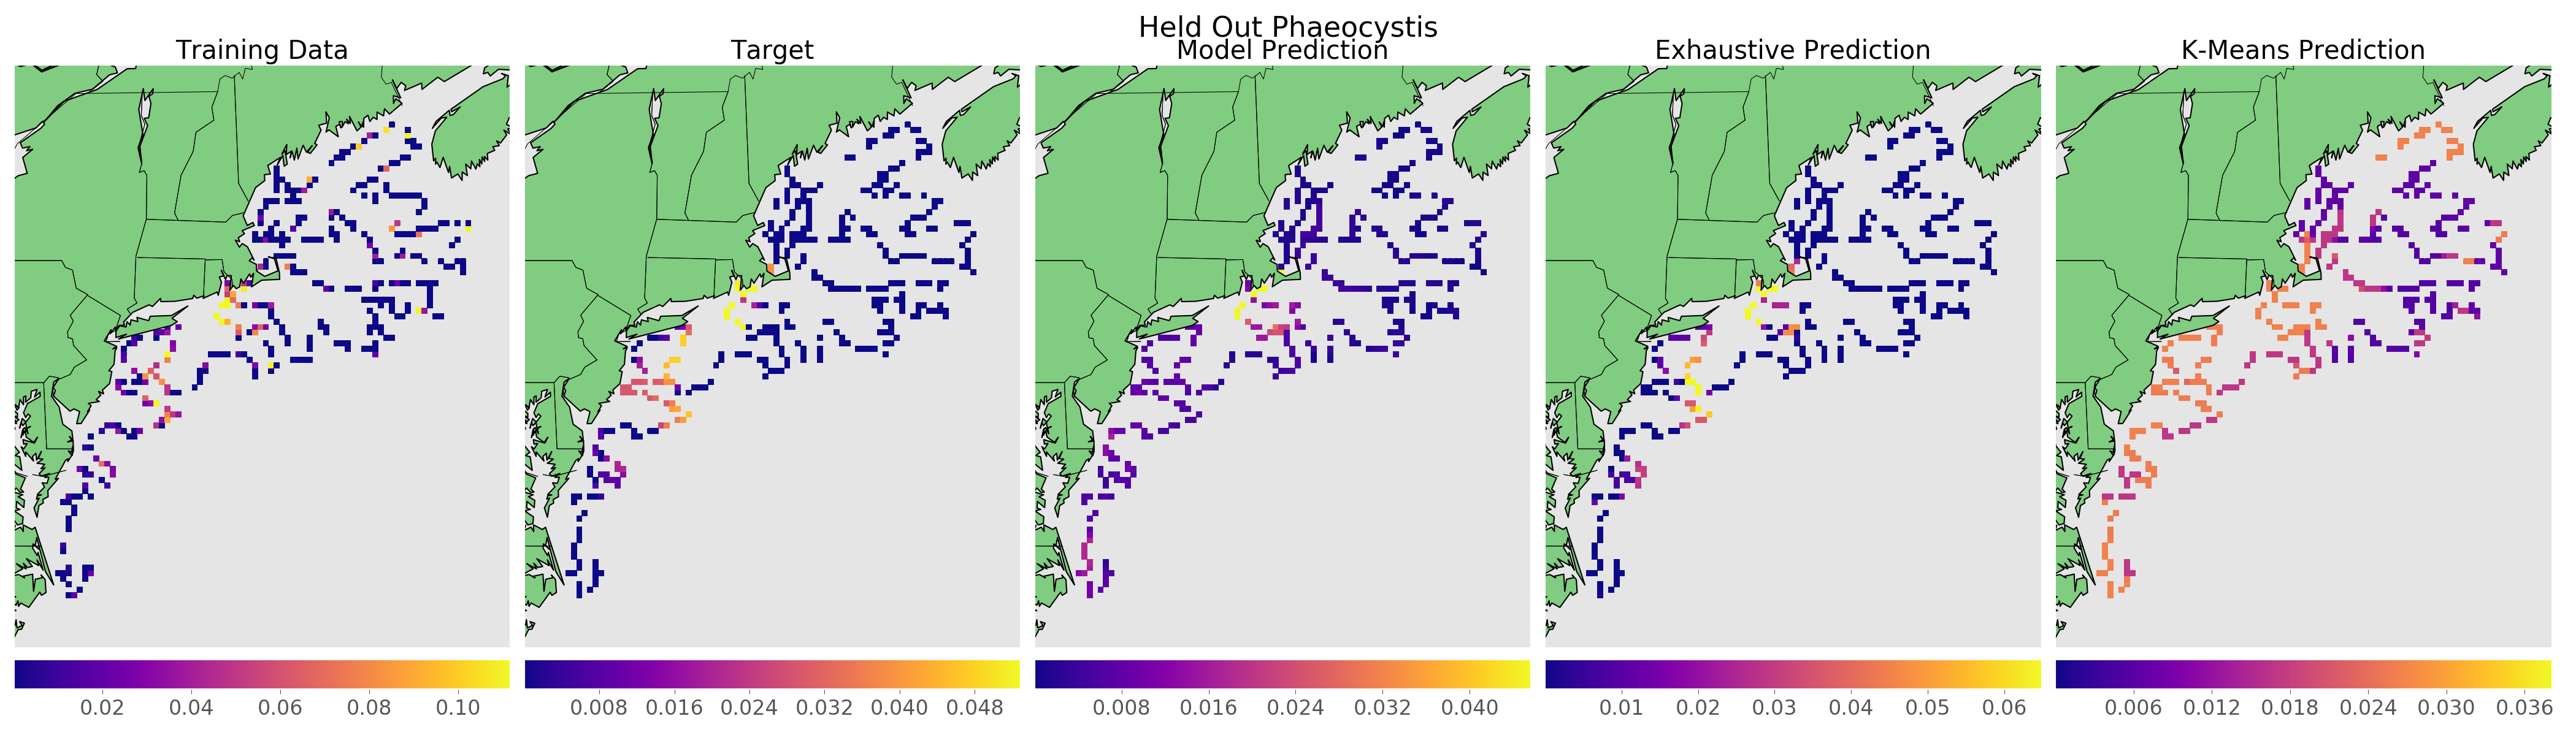
\includegraphics{figures/icra_plankton/maps_Phaeocystis_8}
        \end{tabular}%
    }
    \caption{Spatial distribution for four target classes (rows) in interleaved training/testing samples. The columns correspond to training data (col. 1), held-out target locations (col. 2), and the three models under evaluation (col. 3-5). We find close correspondence between the proposed model and the target data, but exhaustive nearest-neighbor approach has the most similar distribution to held-out target locations. This is because the distribution of plankton is correlated with its spatial neighbors, and hence simple interpolation of the training data is likely to give an accurate plankton distribution at the held-out locations.}
    \label{fig:plankton-pisces-maps-8}
\end{figure}
\begin{figure}
    \centering
    \resizebox{0.9\textwidth}{!}{%
        \begin{tabular}{c}
        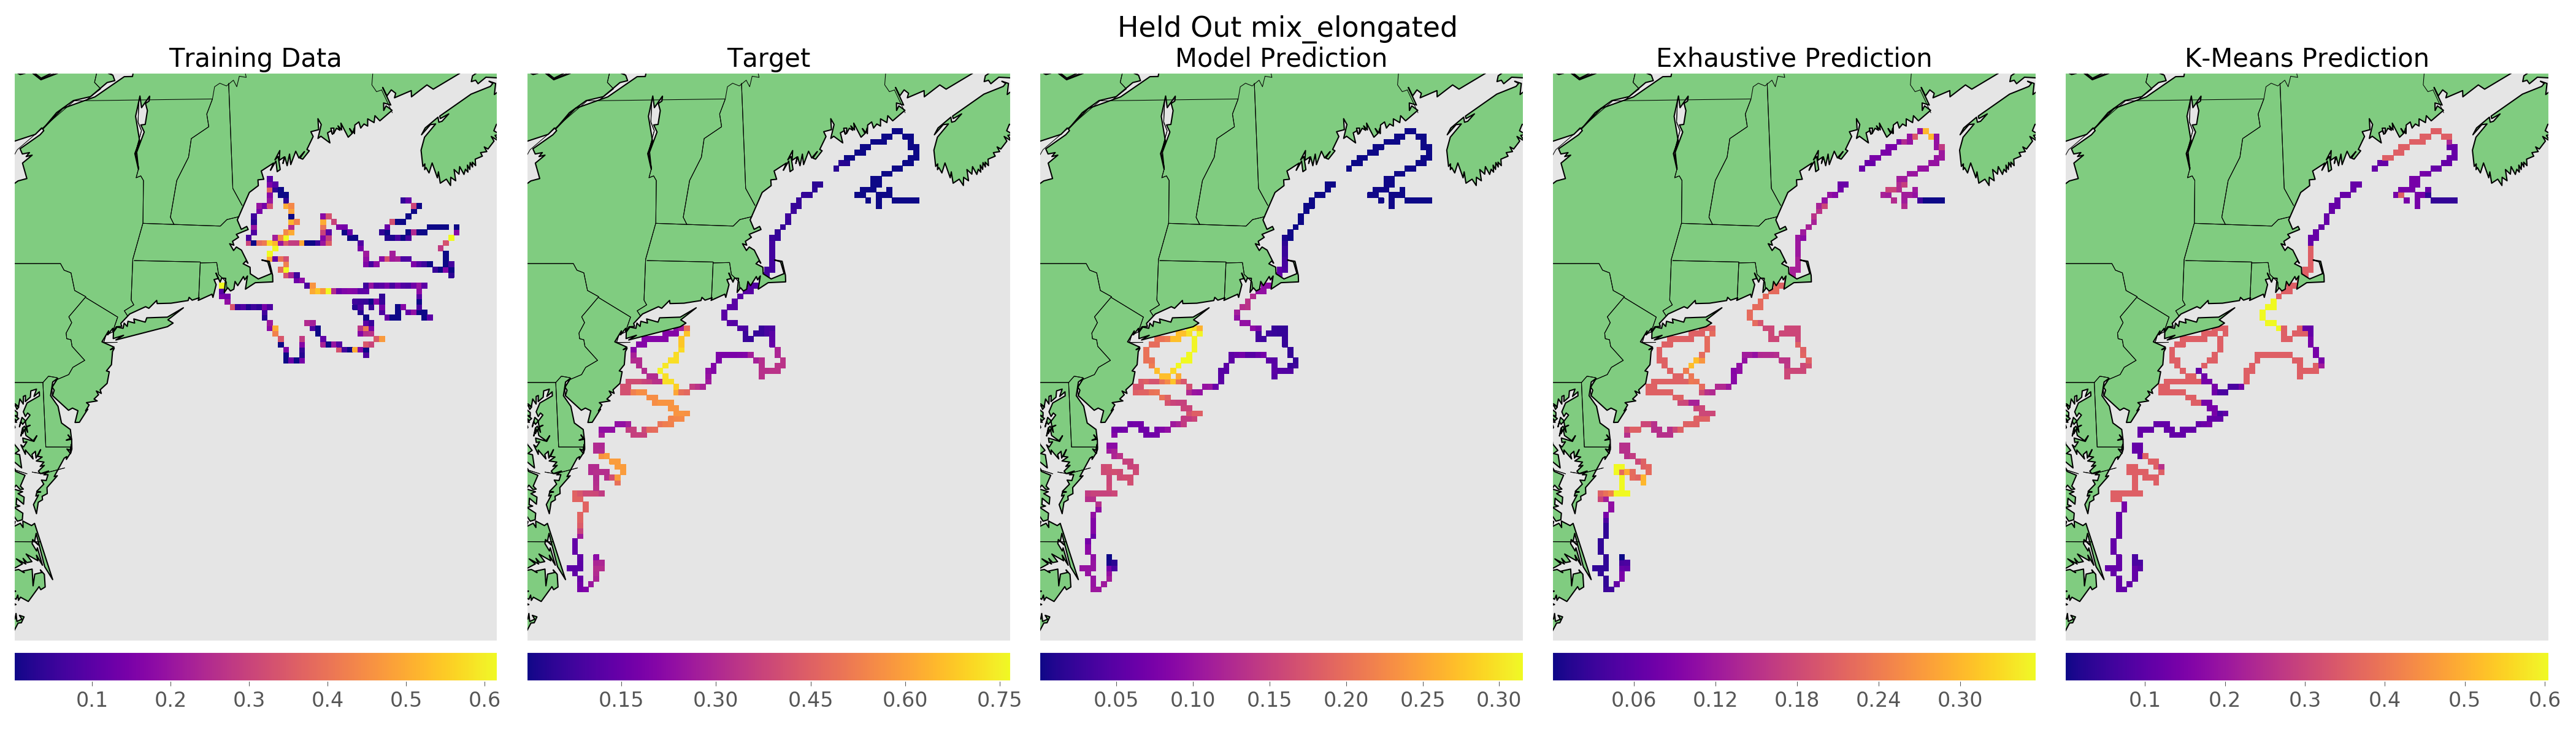
\includegraphics{figures/icra_plankton/maps_mix_elongated_1} \\
        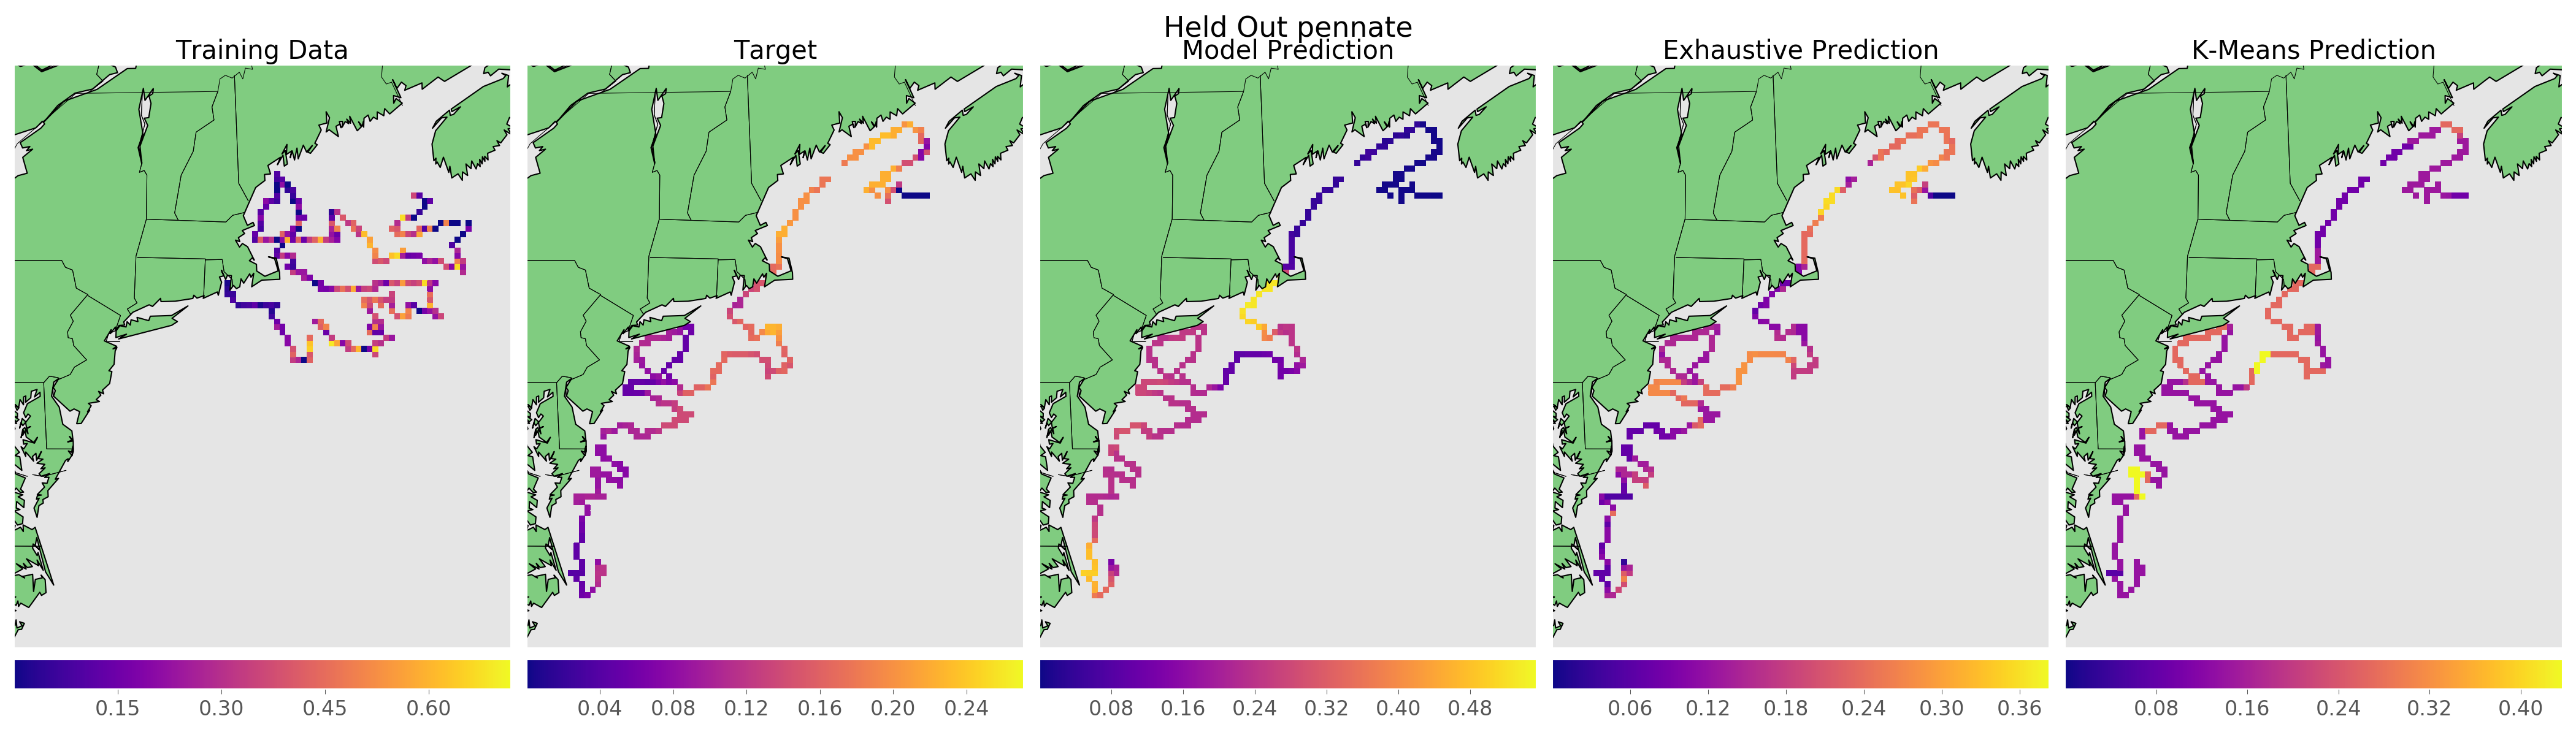
\includegraphics{figures/icra_plankton/maps_pennate_1}\\
        %\includegraphics{figures/icra_plankton/maps_Thalassiosira_1}\\
        % \includegraphics{figures/icra_plankton/maps_Guinardia_1}\\
        % \includegraphics{figures/icra_plankton/maps_Guinardia_striata_1}\\
        \includegraphics{figures/icra_plankton/maps_Dictyocha_1}\\
        \includegraphics{figures/icra_plankton/maps_Ephemera_1}\\
        %\includegraphics{figures/icra_plankton/maps_Phaeocystis_1}
        \end{tabular}%
    }
    \caption{Spatial distribution for four target classes (rows) in split training/testing samples. The columns correspond to training data (col. 1), held-out target locations (col. 2) , and the three models under evaluation (col. 3-5). The proposed plankton topic model provides predictions that agree better with the held-out observations than do the simpler k-means based plankton community model or the exhaustive nearest neighbor search.}
    \label{fig:plankton-pisces-maps-1}
\end{figure}

We ran our model for a range of choices of the hyperparameters $\alpha, \beta \in$ \{0.001, 0.01, 0.1, 0.5, 1\} and $\gamma \in \{10^{-6},10^{-5},10^{-4}\}$ with each of the top 8 taxa held out of the testing data and for both training regimes. We also ran the exhaustive search and k-means strategies for each. The strategies each produce an estimate for $P(w=v^\star | g(x))$, which we then smooth with a median filter with size parameter $\sigma$. For a scalar threshold $\tau$, we predict that location $x$ is a hotspot if $\Pi_\sigma(P(w=v^\star | g(x))) > \tau$, where $\Pi_\sigma$ is the median function over a square region with side length $\sigma$. 

To evaluate our results we compare the held-out locations in the test set (Fig.~\ref{fig:plankton-pisces-maps-8} and \ref{fig:plankton-pisces-maps-1}, column 2) to predictions from each of the proposed strategies (Fig.~\ref{fig:plankton-pisces-maps-8} and \ref{fig:plankton-pisces-maps-1}, our model, column 3; exhaustive nearest neighbour search, column 4; and k-means search, column 5). The input to the models is illustrated with the observed values of the held-out class at the training locations (Fig.~\ref{fig:plankton-pisces-maps-8} and \ref{fig:plankton-pisces-maps-1}, column 1). Our findings show that the prediction problem is relatively straightforward for the interleaved experiment (Fig.~\ref{fig:plankton-pisces-maps-8}). In contrast, the problem is much more difficult when training and testing locations are in different parts of the world. (Fig.~\ref{fig:plankton-pisces-maps-1}). Despite this, for three (Fig.~\ref{fig:plankton-pisces-maps-8} and \ref{fig:plankton-pisces-maps-1}, rows 1, 2, 4) of the four target classes shown here, the spatial location of maxima of our model's predictions are consistently near the maxima in the target distributions.

Varying $\tau$ for each strategy and parameter setting we can count the true positive, true negative, false positive, and false negative hotspot predictions compared to the top 50 examples in the held-out data. These counts give the precision and recall for each parameter choice, for each $v^\star$. We also accumulate these counts across all $v^\star$ to compute the overall precision and recall for each choice of parameters. We assign each set of parameters a score given by the area under its aggregated precision-recall curve and select the parameter set with the maximum score for further comparisons. For the interleaved experiment, best performance was achieved with $\alpha=0.1, \beta=0.1, \gamma=10^{-5}, \sigma=25 km$ and for the split experiment, $\alpha=0.1, \beta=1.0, \gamma=10^{-5},\sigma=35 km$. We chose the number of centroids for the k-means strategy to be the same as the number of topics in the best performing topic model, $K=9$ for the interleaved experiment, and $K=6$ for the split experiment.

We compare the aggregated and individual class precision-recall curves for the best parameters for each strategy (Fig.~\ref{fig:plankton-pisces-pr}). From the aggregated precision-recall curves, we find that our model significantly outperforms the exhaustive nearest-neighbor and the k-means strategies on the split-samples regime, especially for low recall requirements. This indicates that the top few predictions of our model were more likely to be true hotspots than those of the other strategies. The exhaustive nearest-neighbor strategy barely performs better than random guessing on the split regime, yet it performs extremely well on the interleaved regime. This result is expected as the exhaustive strategy does not reason at all about the underlying association between plankton types. Instead, it depends on having observed a training point whose distribution is similar to every test point. In contrast, our model performs nearly as well on the split regime as the interleaved regime.

Our model also outperforms the k-means strategy on the split-samples regime. Note that the k-means strategy is exactly equivalent to the exhaustive search strategy in the limit where $K$ is the number of training points. Both these strategies rely on a distance measure over the class distributions. The high dimensionality of the distributions acts to the detriment of the divergence measure. As the dimensionality of a space increases, the discriminating power of distance metrics within that space decreases. The amount of data needed to find meaningful clusters grows exponentially with the number of dimensions, a phenomenon sometimes called \textit{the curse of dimensionality}. As a result, the two search-based strategies perform well when test points are very near to training points in taxon distribution space, but when test points are further away, a distance measure is less informative and performance is negatively impacted.

\begin{figure}
	\centering
    \begin{minipage}{\textwidth}
        \subfloat[][]{
            \includegraphics[width=\textwidth]{figures/icra_plankton/pr_8.png}
            \label{fig:plankton-pisces-pr8}
        }\\
       \subfloat[][]{
            \includegraphics[width=\textwidth]{figures/icra_plankton/pr_1.png}
            \label{fig:plankton-pisces-pr1}
        }
    \end{minipage}\\
    \begin{minipage}{\textwidth}
    	\centering
        \subfloat[][]{
            \includegraphics[width=0.48\textwidth]{figures/icra_plankton/pr_summary_8.png}
            \label{fig:plankton-pisces-pr8s}
        }%
        \subfloat[][]{
            \includegraphics[width=0.48\textwidth]{figures/icra_plankton/pr_summary_1.png}
            \label{fig:plankton-pisces-pr1s}
        }
    \end{minipage}

    \caption
    {Precision vs recall curves for the community model on each of 8 held-out taxa.
	 \protect\subref{fig:plankton-pisces-pr8}, \protect\subref{fig:plankton-pisces-pr8s} Interleaved train and test data.
	 \protect\subref{fig:plankton-pisces-pr1}, \protect\subref{fig:plankton-pisces-pr1s} Disjoint train and test data.
    }
    \label{fig:plankton-pisces-pr}
\end{figure}

%!TEX root = thesis.tex

\chapter{Spatial Awareness for Robot Cameras: Predicting images from topic context} \label{ch:spatial-prediction}

In this chapter we consider learning a word distribution function which is suitable for topic modelling as well as a function to map such a word distribution back to the original domain. Such a feature representation, combined with a spatio-temporal topic model opens a broad range of applications where we would like to develop a high-level understanding of data in its original domain rather than in a word-like representation. Specifially, we consider modelling the views available to a robotic Pan, Tilt, Zoom (PTZ) camera. Our word distribution function is a novel convolutional autoencoder (CAE), which takes an image as input, produces a distribution of words as its encoding, and then attempts to reconstruct the original image from this encoding. By fitting a topic model within a domain where we can decode word distributions to images, we enable a user of the PTZ camera to inspect the topic distributions $\Phi$ directly as images. These topic images provide an intuitive decomposition of the high-level parts of the scene and a novel interface to explore views by combing them in different proportions.

Further, we employ a similar approach to Ch.~\ref{sec:plankton-seasonal} to recover the word distribution for a neighborhood given its estimated topic prior. Together with the reconstruction function, this enables us to directly view the data captured by the topic model and the data that is lost by constraining ourselves to a sparse, low-dimensional representation. Finally, we develop an energy-based topic-prior mapping model that exploits the spatial smoothness of the learned topic priors to make predictions for unobserved views. Combining all of these pieces together, we develop a system to predict the images the PTZ camera would encounter if it were to configure itself for a novel view.

\section{Learning an invertible word distribution function} \label{sec:learning-features}

\subsection{Background}

Our work on learning an invertible feature function draws from the extensive literature on Deep Convolutional Autoencoders. The simplest version of an autoencoder is a parameterized model, trained to reproduce its inputs with minimal error. Most often, autoencoders adopt a `bottleneck' intermediate representation with many fewer dimensions than the input space; this helps ensure that the model learns a useful representation of the data rather than a trivial one. The bottleneck layer divides an autoencoder into an encoding function $e$ and a decoding function $d$, while the activations for a particular input at the bottleneck layer are its encoding. We will write $I_x$ for the image at point $x$, $h_x = e(I_x)$ for its hidden encoding, and $\hat{I}_x = d(h_x)$ for the `autoencoded' representation of the image through the network. The standard account of autoencoder training considers the random variables $\mathbf{I}$ and $\mathbf{\hat{I}}$ and seeks to minimize $L_{ae} = -\log P(\mathbf{I} | \mathbf{\hat{I}})$ given a modelling choice for $P(\mathbf{I} | \mathbf{\hat{I}})$. When $I$ is considered an unconstrained real-valued tensor, it is common to assume $\mathbf{I}|\mathbf{\hat{I}} \sim \mathcal{N}(\mathbf{\hat{I}}, \Sigma)$, which leads to the standard MSE loss $\mathcal{L}_{ae} = \sum_x \| I_x - \hat{I_x}\|_2^2$, proportional to an unbiased estimator for $L_{ae}$ \citep{vincent2010stacked}.

A key strength of autoencoder models is that the only training data they require are the images themselves, and therefore large datasets are relatively easy to produce. Because of this, as larger, more elaborate, supervised CNN architectures have improved and the availablility of high-performance GPUs has increased, it has become tempting to use the similarly large networks for to get more exact autoencoders without increasing bottleneck sizes. It is often the case, however, that a very powerful decoder will learn to largely ignore the inputs and their encodings and instead memorize a few indistinct outputs to use for every input, eventually learning identical encodings for all inputs \citep{vincent2010stacked,Chen2016}\footnote{This problem has been discussed most prominently under the name `posterior collapse' within the Variational Autoencoder literature, referring to models that learn $e$ as an approximate posterior $q(h | I) \approx p(h)$.}. In the applications discussed in this chapter, avoiding such collapsed encodings is crucial -- for the topic model to learn the spatial arrangement of the scene the learned feature representation should encode as much about the differences between images as possible rather than deferring to the decoder network. Many recent models partially solve this problem by using recurrent networks rather than single-shot encodings to progressively encode and refine their representations, for example \citep{OordPixelCNN,Chen2016,Gregor2016}. These approaches have achieved some of the most visually convincing results to date, especially in the domain of high-resolution image encodings. These methods are not, in principal, exclusive with ours, however they add significant complexity to the possible set of architectures, so we choose to address this issue by other means.

Beyond the common collapsed encoder issue, the most notable novel requirement for our feature encoding is that features must be discrete-valued, whereas most autoencoders produce real-vector valued encodings. Discrete-valued autoencoder representations have been previously considered in the context of image compression by \citep{AgustssonSoftToHardVQ,vqvae2017}. Both of these approaches rely on vector-quantization based on a codebook (fixed beforehand by \citep{AgustssonSoftToHardVQ} and learnt by \citep{vqvae2017}) of closest centers to discretize the encoding space. In contrast, we design an autoencoder model where the latent space is taken to be the parameter of a categorical or multinomial random variable. This has the advantage of fitting directly with the histogram of words document model assumed by LDA, while simultaneously considerably simplifying the required modifications to standard autoencoder architectures to achieve discretization.

\subsection{Categorical Information Boost Autoencoder -- CIB-AE}

In order to learn a representation compatible with topic modelling, we develop a modified CAE, the Categorical Information Boost Autoencoder (CIB-AE), where the encoding can be seen as the parameter of a multinomial distribution so that it gives an image's word distribution directly. We consider encoding an image by the normalized histogram of $N$ `words' -- the learned visual primitives which we can use to reconstruct an image -- drawn from this distribution (Fig.~\ref{fig:cibae-words} presents decodings of single words). Similar to DNNs used for classification tasks, we simply apply the softmax function to the activations of a standard CNN architecture to produce such a distribution. In doing so, we discretize the feature space by considering each dimension of the representation as a discrete `word', and preserve detail in our model by modelling the full feature distribution directly.

\begin{figure}
    \subfloat[][]{
        \includegraphics[width=0.3\textwidth]{figures/ptz/words_spatial}
        \label{fig:words-spatial}
    }
    \subfloat[][]{
        \includegraphics[width=0.6\textwidth]{figures/ptz/top_words}
        \label{fig:words-top}
    }
    \caption{CIB-AE decodings of single `words', i.e. one-hot encoding vectors. An image is reconstructed as a normalized word-histogram.
             \protect\subref{fig:words-spatial} Each word is duplicated at $4 \times 4$ spatial locations within a $128 \times 128$ input image.
             \protect\subref{fig:words-top} The top 128 most common words from the training set, at their central position.}
    \label{fig:cibae-words}
\end{figure}

Through the Dirichet priors on topics and topic-word distributions, LDA descendants such as the spatio-temporal topic model make the implicit assumption that documents have sparse word distributions. Although we do not specify exactly how sparse such a sparse mixture of sparse multinomials is, we have found in practice that simply renormalizing the features of conventional autoencoders produces word-distributions that are too uniform to be modelled productively by LDA. Therefore, CIB-AE employs an additional regularization term in its loss,
\begin{equation}
    L_{CIB} = -\log P(\mathbf{I} | \mathbf{\hat{I}}) - \lambda MI\left(\mathbf{I}, W\right)
\end{equation}
where $W \sim e(I)$ and $MI$ stands for the mutual information, a measure of the degree of dependence between two random variables. Choosing a large value for $\lambda$ will result in representations that favor high mutual information between images and encoding distributions, i.e. those where training images are as distinguishable as possible in encoding space. On the other hand, choosing a small $\lambda$ will result in encodings which may be very similar, but result in a low MSE. In other words this regularization term ensures that encoder collapse does not occur as it does with many other autoencoders \footnote{We note an interesting connection to the literature on VAEs, which uses an approximate prior $q(W|\mathbf{I}) \approx p(W)$. Rewriting $MI\left(\mathbf{I}, W\right)$ as $D_{KL}[(I,W) \| IW ]$, our objective and the VAE objective take extremely similar forms: In particular, $L_{CIB} = -\log p(\mathbf{I} | \mathbf{\hat{I}}) - \lambda D_{KL}[(\mathbf{I},W) \| IW ]$ while $L_{VAE} = -\log p(\mathbf{I} | \mathbf{\hat{I}}) + \lambda D_{KL}[q(W|\mathbf{I}) \| p(W) ]$.} \footnote{Note that in the context of standard normal priors for the latent space, denoising autoencoders \citep{vincent2010stacked}, i.e. autoencoders with dropout, can be considered to enhance the MI between images and encodings as well.}.

To illustrate how our loss works, consider another way to rewrite the mutual information: $ MI\left(\mathbf{I}, W\right) = H[W] - H[W | \mathbf{I}] $ where $H[W | \mathbf{I}]$ signifies the conditional entropy. By subtracting the mutual information from the loss, the $H[W | \mathbf{I}]$ term ensures that individual encodings must have low entropy, and are therefore sparse, while the $-H[W]$ term ensures that the overall distribution of encodings is high entropy, and therefore as uniform as possible. The combination of these two terms means that the encodings must use different dimensions of the feature space from one another.

Reorganizing the mutual information in this also way reveals how to estimate it from a minibatch of size $M$:
\begin{equation}
\begin{split}
    -MI\left(\mathbf{I}, W\right) = H[W | \mathbf{I}] - H[W] = \\
    \mathbb{E}_{w \sim e(I)}\left[ -\log p(w) \right] - \mathbb{E}_\mathbf{I}\left[ \mathbb{E}_{w \sim e(I)}\left[ -\log p(w) \right] \right] \approx \\
    -\frac{1}{M} \sum_{m=1}^M \sum_{d=0}^V e(I_m)_d (\log e(I_m)_d) +
            \sum_{d=0}^V \overline{h}_d \log \overline{h}_d
    \end{split}
\end{equation}
where $\overline{h}$ signifies the average encoding for the $M$ images in the batch. Clearly, estimating an expectation over the space of all possible training images with a minibatch of few dozen or at most a few hundred examples is crude. Nevertheless, the terms of this approximation naturally fit our goal of producing maximally sparse, maximally distinct encodings for as much of the training data as possible. To summarize our approximation of the CIB loss
\begin{equation}
L_{CIB} \approx \mathcal{L}_{CIB} = \frac{1}{M} \left( \sum_{i=1}^M \frac{(I_m - \hat{I}_m)^2}{|I|}
                                    - \lambda \sum_{d=0}^V e(I_m)_d (\log e(I_m)_d) \right)+
                                     \lambda \sum_{d=0}^V \overline{h}_d \log \overline{h}_d
\end{equation}
where $|I|$ denotes the (fixed) number of pixel for an input image. In other words our loss is the MSE plus the average entropy of all encodings, minus the entropy of the average encoding. We find in practice that when the image space is normalized to the range $[-a,a]$, $\lambda = \frac{(2a)^2}{\log V}$ is a good choice, where $V$ is the dimension of the encodings \footnote{Note $\log V$ is the maximum possible entropy for a categorical distribution of dimension $V$, so this choice represents letting the MSE and MI terms have `equal' weight when both are in their worst cases}.

Our specific choice of architecutre is inspired by the feature layers of VGG \citep{Simonyan14c}. In particular, following the approach of Segnet \citep{BadrinarayananK15} we choose a VGG-like encoder, with a symmetric decoder of transposed convolutional layers. This style of encoder uses a sequence of convolution `blocks', which each ultimately either downsample (Max Pool) or upsample (Nearest Neighbor) the activations by a factor of two. We add an additional dropout and an additional softmax layer to the encodings to constrain the real-valued activations of a Segnet style encoding to a simplex. Our feature representation downsamples the image spatially by a factor of 32, while producing a 512 channel feature activation for each spatial region. All experiments are conducted with $128 \times 128 \times 3$ input images, resulting in $4 \times 4 \times 512 = 8192$ dimensional encodings distributions. The full details of our architecture are found in App.~\ref{ch:cibae-arch}, however we emphasize that by adding these two extra layers and the additional loss term, our approach can potentially be transferred to many domains and existing autoencoder architectures.

\section{Spatial topic prediction model}

Beyond simply finding any low-dimensional representation of the image space a PTZ camera may encounter, the spatio-temporal topic model is able to learn such a representation that is also spatially coherent. We situate the topic model's neighborhoods in the space of views, meaning that the resulting learned topic priors will form a map of the visually distinct regions in pan-tilt-zoom space.

Because our model is designed to make the topic priors locally smooth, we are able to develop a simple spatial prediction scheme for topic priors. Our spatial prediction model is fast to fit and run online, taking camera pose, learned topic prior pairs as training data, and predicting the topic prior for a test pose. We take inspiration from a nearest-neighbor model: in the simplest case our approach is to predict the topic prior of the nearest training point for a test point. We envision using this system with only a few dozen training points, and would prefer predictions to degrade towards the global average topic distribution than a poor estimate of the topic prior when the test point is not near any training point.

To achieve this property, we implement our predictions using an energy-based model, using a weighted sum over the topic distributions we have observed so far, where far training points have low weight and near training points have high weight. Rather than performing such a prediction with a direct mixture of observed topic-priors and renormalizing, we choose to implement the weighted sum in terms of the log-probability of each training topic, and then use a softmax to return to the natural probability space. We found that in practice, this approach helps to maintain sparcity of predicted topic priors, a property assumed by the topic model. Note that if the mixture of log-probabilities belongs to a valid probability distribution (\emph{eg.} all the weight is placed on a single training point), the softmax function returns exactly that distribution.

We define the weights in terms of a Boltzmann distribution (i.e. the softmax of negative energy), using the distance to each observed topic prior as the energy. Let $D_X(x)$ denote the distance vector from point $x$ to each point in the training set $x_i \in X$. This choice of weight function has the appealing property that if any entry of $D_X(x)$ is much smaller than the rest, all of the weight will be put on that training point. Further, with this weight function, by controlling the scale of the distances we can control the sparsity of the weight vector; when the average distance is low the weights will be fairly uniform, while when the average distance is high, the weights will be sparser. We choose to use the $\mathit{L}_2^2$ distance between pan-tilt-zoom points as our distance function. In order to appropriately scale the distances and balance dimensions which may not truly incur equal loss of relevance for higher distances, we first scale the input points by the vector $w$ \footnote{Our distance could also be called a Mahalanobis distance (normally formualted in terms of the covariance matrix $\Sigma = ww^T$)}. To summarize our prediction model, given $N$ training points $X$ each paired with an observed topic prior in $\Theta_X$:
\begin{equation}
\begin{split}
    D_X(x) = 
    \begin{bmatrix}
    \|w^Tx - w^T x_1 \|_2^2, & \|w^Tx - w^T x_2 \|_2^2, \ldots, \|w^Tx - w^T x_N \|_2^2
    \end{bmatrix}^T\\
    W(x) = \sigma \left( -D_{X}(x) \right)\\
    \theta(x) = \sigma \left( \log \left(\Theta_X \right) W(x) \right)
\end{split}
\end{equation}

Finally, we note that setting $w$ by hand is difficult as the best choice may vary from environment to environment, and is unnecessary, as both fitting and prediction are extremely efficient with this model. Instead, given a validation set $X^\star, \Theta^\star$ held out of training, we consider the information lost by using our model, measured by the mean Jensen-Shannon Divergence on the validation set:
\begin{equation}
L_w = \frac{1}{|X^\star|} \sum_{x \in X} D_{JS}\left[\theta(x) \| \Theta^\star_x \right]
 =  \frac{1}{|X^\star|} \sum_{x \in X} \frac{1}{2} \left(D_{KL}\left[\theta(x) \| m(x) \right] + D_{KL}\left[\Theta^\star_x \| m(x) \right]\right)
\end{equation}
where $m(x) = \frac{\theta(x)+\Theta^\star_x}{2}$. While $D_{KL}\left[\theta(x) \| \Theta^\star_x \right]$ would most directly measure the information lost by approxmating the true topic distribution with the prediction, $D_{JS}$ is additionally symmetric, positive, and bounded above, making it a more convenient loss function. This loss and our model are differentiable, so we are able to fit $w$ using gradient descent and a 2-fold cross-validation procedure. As a final note, although a more complex distance model may better match how topic-priors are spatially distributed, because we aim to train this model with only a few dozen examples we prefer a simpler model that is less prone to overfitting.

\section{Experiments}

\subsection{Simulated Pan-Tilt-Zoom Camera Dataset}
\begin{figure}
    \centering
    \includegraphics[width=0.85\textwidth]{figures/ptz/sun360_9x.jpg}
    \caption{Example 360 degree panoramas from the SUN360/street dataset.}
    \label{fig:sun360_ex}
\end{figure}

We demonstrate our approach with a simulated outdoor pan-tilt-zoom camera, using data from the `street' category of the SUN360 dataset \citep{SUN360}. Specifically SUN360/street comprises a dataset of 161 360 degree panoramas projected into rectangular $9104 \times 4552$ pixel images (Fig.~\ref{fig:sun360_ex}). These panoramas are taken in various cities and towns across the world, from street corners and from car-mounted cameras. The data are pre-processed tso that the horizon is horizontal and vertically centered in all panoramas. We parameterize views in terms of tilt angle $T$, pan angle $P$, zoom factor $Z$. Given a base field-of-view (fov) $A_0$ and a target camera resolution, we compute the projection to the desired perspective $R = R_TR_P$ where
\begin{equation}
\begin{split}
R_T =& 
\begin{bmatrix}
1 & 0 & 0\\
0 & \cos(T) & -\sin(T)\\
0 & \sin(T) & \cos(T)
\end{bmatrix}\\
R_P =&  
\begin{bmatrix}
\cos(P)        & \sin(P) - \sin(T)            & \sin(P)\cos(T)\\
\sin(P)\sin(T) & \cos(P)\cos(T)^2(1 -\cos(P)) & \cos(T)\sin(T)(1-\cos(P))\\
\sin(P)\cos(T) & \sin(T)\cos(T)(1-\cos(P))    & \cos(P)+\sin(T)^2(1-\cos(P))
\end{bmatrix}
\end{split}
\end{equation}
Using the fov $A = A_0/Z$ and fixed output image resolution, we represent each output pixel location as a pan-tilt rotation from the center $P$, $T$. Then, projection proceeds as rotation by $R$ and a lookup in the full panorama image for each pixel in the output image. In all our experiments we consider a base fov of 76 deg and zoom factors $Z \in [1, 12]$, similar to a standard commodity camera. Further, to avoid wrapping angles, we consider only $T \in [-60, 60]$ and $P \in [-120, 120]$ degrees.

\subsection{Place-specific autoencoder}
A key advantage of the topic-model based approach is that it can be trained online, whereas this is not practical for large deep-networks. This means that rather than learning a single model which aims to produce a low-dimensional embedding of all possible images, our robotic camera system can learn a new, place specific model which is thus required to represent a vastly simpler image space, and thus is significantly faster and more reliable to train.

\subsubsection{CIB-AE Training}
\begin{figure}
    \centering
    \includegraphics[width=\textwidth]{figures/ptz/mc3ae_encodings}
    \caption{Random example input images (left) and CIB-AE reconstructions (right) for 4 worlds (rows) from the SUN360/street test set.}
    \label{fig:cibae_encodings}
\end{figure}

\begin{figure}
    \centering
    \includegraphics[width=0.95\textwidth]{figures/ptz/word_frequency}
    \caption{Word-distribution, sorted by frequency, of the average encoding over 1000 test images (heavy black line) and normalized
             word-histograms for 3 random images (colored lines). A uniform histogram over the 8192 dimensions (dashed black line) represents the ideal average encoding and the worst-case individual encoding.}
    \label{fig:cibae-words-distribution}
\end{figure}

Our approach delegates learning the globally-salient image embedding to the CIB-AE. In particular, we trained our feature model using epochs of 5000 random views from amongst 80 SUN360/street panoramas. We found that choosing a new set of random training views for each epoch was crucial, however we kept the validation set fixed throughout training. The projection described in the previous section is time consuming for high-resolution images, especially for those that do not fit in GPU memory. Therefore we trained for 175 epochs on random square crops from the warped panorama images, and then 25 more epochs on projections to fine-tune the results. We achieved our results using the adaptive learning rate optimizer Adam~\citep{KingmaAdam}, however found that a learning rate decay by a factor of 0.9 every 10 epochs was also necessary. Example input images and their autoencoded counterparts can be seen in Fig.~\ref{fig:cibae_encodings}. We found the mean entropy of image encodings from 1000 random views from the test set to be 6.170 nats \footnote{While bits is the unit for information measured by entropy using $log_2$, nats is the unit when the entropy is calculated using $ln$}, or approximately equivalent to a uniform PMF over just 470 dimensions. On the other hand, the entropy of the mean encoding distribution from these 1000 examples was 8.192 nats, whereas the maximum possible entropy where all feature dimensions were used uniformly would have had an entropy of 9.011 nats. Typical word distributions and the average word distribution are illustrated in Fig.~\ref{fig:cibae-words-distribution}.

\subsubsection{View Prediction}
We train our view-predictor by alternating between observing new encoding distributions and refining a spatio-temporal topic model for a fixed period of 1 second. At the end of each refinement phase the spatial topic map is refit using normalized pan, tilt, and zoom-factor spatial coordinates and a corresponding point-estimate of the posterior for $\Theta$ given the topic assignment counts. Then, the partially trained spatial topic-prior map can be used to select the next training view (discussed in Sec.~\ref{sec:active-learning}) or it can be chosen uniformly at random.

When the image corresponding to the new view is extracted its word distribution is computed based on our trained CIB-AE. Because our Gibbs sampling inference method samples from the posterior for the topic assignment of a single word given all the others, it is necessary to discretize the encoding distribution by sampling from it rather than work with it directly. Note that despite an encoding dimension of 8192, it is possible to use a relatively small number of discrete observations without losing detail because individual images have low entropy encodings. In our experiments we define a constant encoding resolution of 3000 words per image; initial experimentation showed some degradation of performance below this level and little improvement above, however clearly the document size defines a tradeoff between the required number of sampling iterations and the amount of detail modelled.

We choose a spatio-temporal topic model with $K = 25$ topics and neighborhoods of size 10 degrees $\times$ 20 degrees $\times$ 6 (tilt $\times$ pan $\times$ zoom). This neighborhood size choice corresponds to the intuition that environments are semantically `smoother' in pan than tilt, and much smoother while zooming than moving the camera. We chose concentration parameter values $\alpha = 0.2,~\beta = 0.2$. We performed extensive cross validation to select these hyerparameter values and certain other choices were found to perform much better for particular environments, however we did not find a combination of hyperparemeter values that was definitively much more performant than the others on average.

\subsection{Spatio-Semantic Image Encoding Results}

Since we aim to demonstrate a real-time system that can learn about its surroundings relatively quickly, we stop learning after 50 observations. As a first inquiry into what the model has learned, we directly decode the point estimates of the topic distributions $\hat{\Phi}$ by passing them through the CIB-AE decoder (See Figs.~\ref{fig:pano-0-topics},~\ref{fig:pano-1-topics},~\ref{fig:pano-2-topics}). Most other applications of visual topic models employ non-invertible feature functions and choose to inspect topics by looking at the most representative training images. To our knowledge, this is the first application of a visual topic model where the topics can be fully decoded and inspected directly as images. Interestingly, we find that for our autoencoder network, sparser encodings produce clearer images, while more uniform encodings produce muddled, mostly gray, blurry images (See Fig.~\ref{fig:map_vs_mle_topics}). This motivates us to use a \emph{maximum a posteriori} (MAP) point-estimate for $\hat{\Phi}$ (as well as for $\hat{\Theta}$) as opposed to the MLE discussed in Eqn.~\ref{eqn:mle_thetaphi}
\begin{equation} \label{eqn:map_thetaphi}
\begin{split}
\hat{\Theta}_{g(x), k} =&
    \begin{cases}
        \frac{N^k_{g(x)} + \alpha - 1}{\sum_{j=1}^K N^j_{g(x)} + \alpha - 1} & if~N^k_{g(x)} > 0 \\
        0 & otherwise
    \end{cases} \\
\hat{\Phi}_{k, w_i} =&
    \begin{cases}
        \frac{N^{w_i}_k + \beta - 1}{\sum_{v=1}^V N^v_k + \beta - 1} & if~N^k_{g(x)} > 0 \\
        0 & otherwise
    \end{cases}
\end{split}
\end{equation}

\begin{figure}
    \centering
    \subfloat[][]{
        \includegraphics[width=0.4\textwidth]{figures/ptz/map_topics.png}
        \label{fig:map_topics}
    }
    \subfloat[][]{
        \includegraphics[width=0.4\textwidth]{figures/ptz/mle_topics.png}
        \label{fig:mle_topics}
    }
    \caption{MAP \protect\subref{fig:map_topics} vs MLE \protect\subref{fig:mle_topics} point estimates for $\Phi$ trained with identical datasets, directly decoded as images. Note that the MAP estimate features more distinctive topic images.}
    \label{fig:map_vs_mle_topics}

\end{figure}

Prediction with our spatial topic prior model is extremely efficient, so we predict the topic priors for 10,000 random $P,T,Z$ views. In Figs.~\ref{fig:pano-0-map}, ~\ref{fig:pano-1-map}, and ~\ref{fig:pano-2-map} we present the resulting topic prior maps (one scatter plot per topic, in the same arrangement as the topic images), with the point $x_i$ omitted for topic $k$ if $\theta(x_i)_k < 0.01$, blue indicating $\theta(x)_k = 0.01$ and red $\theta(x)_k = 1$. Together, the decoded topics and view-topic maps provide an evocative graphical representation of how low-level textures combine into a higher level scene structure. After training, we collected 50 more views along with their inferred MAP topic priors (without performing any more refinement of $\Phi$). Among these observed views for each of the 35 test panoramas, we found $D_{JS}[\theta(x), \hat{\theta}]$ to be on average 0.1953 nats, while $D_{JS}[\mathrm{Unif}(K), \hat{\theta}]$ was on average 0.5122 nats\footnote{Recall $0 \leq D_{JS} \leq \ln(2) \approx 0.6931$}. This indicates that the topic mapping procedure is imperfect as is expected because of its weak geometric assumptions, however it does capture a significant portion of the information about the spatial distribution of topics.

\begin{figure}{}{}
    \centerline{
    \begin{minipage}{0.6\textwidth}
        \subfloat[][]{
            \includegraphics[width=\columnwidth]{figures/ptz/pano_0_topics.png}
            \label{fig:pano-0-topics}
        }
    \end{minipage} \hfill
    \begin{minipage}{0.6\textwidth}
        \subfloat[][]{
            \includegraphics[width=\columnwidth]{figures/ptz/pano_0_map.png}
            \label{fig:pano-0-map}
        } \\
        \subfloat[][]{
            \includegraphics[width=\columnwidth]{figures/ptz/pano_0_pano.jpg}
            \label{fig:pano-0-pano}
        }
    \end{minipage}
    }
    
    \caption{Example spatial prediction model after 50 training observations. \protect\subref{fig:pano-0-pano}} Fish-eye view of the entire panorama \protect\subref{fig:pano-0-topics}, Direct decoding of each topic-distribution ($\Phi_k$), And \protect\subref{fig:pano-0-map} predicted mixture of each topic.
    \label{fig:pano-0}
\end{figure}

\begin{figure}
    \centerline{
    \begin{minipage}{0.6\textwidth}
        \subfloat[][]{
            \includegraphics[width=\columnwidth]{figures/ptz/pano_1_topics.png}
            \label{fig:pano-1-topics}
        }
    \end{minipage} \hfill
    \begin{minipage}{0.6\textwidth}
        \subfloat[][]{
            \includegraphics[width=\columnwidth]{figures/ptz/pano_1_map.png}
            \label{fig:pano-1-map}
        } \\
        \subfloat[][]{
            \includegraphics[width=\columnwidth]{figures/ptz/pano_1_pano.jpg}
            \label{fig:pano-1-pano}
        }
    \end{minipage}
    }
    
    \caption{Example spatial prediction model after 50 training observations. \protect\subref{fig:pano-1-pano}} Fish-eye view of the entire panorama \protect\subref{fig:pano-1-topics}, Direct decoding of each topic-distribution ($\Phi_k$), And \protect\subref{fig:pano-1-map} predicted mixture of each topic.
    \label{fig:pano-1}
\end{figure}

\begin{figure}
    \centerline{
    \begin{minipage}{0.6\textwidth}
        \subfloat[][]{
            \includegraphics[width=\columnwidth]{figures/ptz/pano_2_topics.png}
            \label{fig:pano-2-topics}
        }
    \end{minipage} \hfill
    \begin{minipage}{0.6\textwidth}
        \subfloat[][]{
            \includegraphics[width=\columnwidth]{figures/ptz/pano_2_map.png}
            \label{fig:pano-2-map}
        } \\
        \subfloat[][]{
            \includegraphics[width=\columnwidth]{figures/ptz/pano_2_pano.jpg}
            \label{fig:pano-2-pano}
        }
    \end{minipage}
    }
    
    \caption{Example spatial prediction model after 50 training observations. \protect\subref{fig:pano-2-pano}} Fish-eye view of the entire panorama \protect\subref{fig:pano-2-topics}, Direct decoding of each topic-distribution ($\Phi_k$), And \protect\subref{fig:pano-2-map} predicted mixture of each topic.
    \label{fig:pano-2}
\end{figure}

In addition to decoding the topic distributions themselves, we can predict the topic prior for a view and the corresponding encoding distribution given the topic distributions, and decode these predicted encodings. We evaluate our system based on the root mean squared error (RMSE) pixel value between the predicted images and the true image at that view. We call views that where we have run topic inference and topic map training but not topic refinement `observed'. At observed views our model predicts exactly the topic prior observed in that location, and so is able to represent the information encoded in the topic model without external loss.

As performance baselines, we trained two additional autoencoders with similarly constrained latent spaces offline, on the SUN360/street training set used to train the CIB-AE. First, we trained a plain CAE, without a categorical distribution latent space or additional loss terms beyond the MSE. We copy the architecture of the CIB-AE up to the softmax layer, and then add 3 additional fully connected layers of sizes 4096, 2048, and 1024, with ReLU and BatchNorm nonlinearities and with a final latent representation of 25 dimensions to complete the encoder. As with CIB-AE, the decoder is symmetric with the encoder. We initialilzed the weights of the encoder by copying them from the pretrained CIB-AE where possible, and trained the CAE using the same procedure as the CIB-AE.

In addition, we trained the previously mentioned vector-quantized variational autoencoder (VQ-VAE) of \citep{vqvae2017} with a codebook of size $25 \times 8192$, identical to the size of the topic model's $\Phi$ parameter. VQ-VAE is a state of the art discrete-latent autoencoder model designed to address many of the same issues as the topic model, however it cannot be trained online like the topic model, and so it must fit a globally salient representation into the fully compressed $25$-dimensional encoding sapce. We found that VQ-VAEs are very sensitive to architecture choices. For a fair comparison, it would be preferrable to use a VQ-VAE with spatial resolution $4 \times 4$ and feature size $512$ for each spatial block, however we could not escape encoder collapse using this representation. In fact, the only spatial resolution we found that attained reasonable results was the one the original authors demonstrated, therefore our comparisons are against a VQ-VAE with spatial resolution $32 \times 32$ and a feature size of just $8$ for each spatial block.

For the baseline approaches, we apply a similar energy-based prediction model as for the topic-priors, however as the encodings are not probability distributions, we mix them by performing the weighted sum directly rather than in log-probability space. In addition, the cross-validation metric for $w$ is the MSE of the predicted encodings rather than $D_{JS}$. Note that the baselines are not trained with spatial information, so we would not expect this method to achieve the same performance as with the spatially smooth topic model.

Fig.~\ref{fig:encoding-obs-strip} shows examples of the autoencoding performance of the various systems through their 25 dimensional representations. The leftmost column is the observed image and the second column is the CIB-AE autoencoding of that image. The subsequent columns are the decoded neighborhood-word distribution, the VQ-VAE autoencoding, and the CAE autoencoding. The CAE is not able to capture any detail in this regime, the gray images seen are characteristic of the encoder collapse problem mentioned previously. The VQ-VAE, unsurprisingly because of its high-spatial resolution and low feature dimensionality, captures the spatial structure of the image relatively well, but loses much of the color and distorts the texture. Finally, our approach is competetive with the VQ-VAE, featuring images that are more spatially distorted, but interestingly, that enhance the color contrast of its input images. Fig.~\ref{fig:encoding-pred-strip} is similar, however it shows unobserved views, predicted through the topic prediction model (For many more examples, see App.~\ref{ch:app-predictions}).

\begin{figure}
    \begin{center}
    \subfloat[]{
        \includegraphics[width=0.89\columnwidth]{figures/ptz/train_stacked_intext.png}
        \label{fig:encoding-obs-strip}
    }\\
    \subfloat[]{
        \includegraphics[width=0.89\columnwidth]{figures/ptz/test_stacked_intext.png}
        \label{fig:encoding-pred-strip}
    }
    \end{center}
    \caption{Observed \protect\subref{fig:encoding-obs-strip} and predicted encodings \protect\subref{fig:encoding-pred-strip} for random views from SUN360/street. From left to right the columns represent true image, CIB-AE autoencoding, topic prediction autoencoding, VQ-VAE latent prediction autoencoding, and plain CAE autoencoding. Many more examples are found in App.~\ref{ch:app-predictions}).
    }
    \label{fig:encoding-strip}
\end{figure}

Fig.~\ref{fig:vs_vqvae} shows the RMSE for observed and predicted topic priors decoded as images compared to the real images at the corresponding views. The low extent of the CAE whisker reveals that the conservative collapsed strategy of consistently predicting uniform grayish images is not necessarily bad in terms of pure pixel error, drawing out an important flaw of the pixel error as a performance measure at this level of compression. Nevertheless, to the extent that the RMSE distributions measure performance in our view prediction task, the data confirm our qualitative assesment that our method performs approximately as well as the VQ-VAE on average, and the extent of its typical errors is lower. Further, the more colorful, highher contrast images produced by our method are reflected by its higher variance than the more conservative VQ-VAE approach which tends to encode roughly the right shape, but obscure much of the color and texture.

\begin{figure}
    \begin{center}
    \subfloat[]{
        \includegraphics[width=0.48\columnwidth]{figures/ptz/vs_vqvae_obs.png}
        \label{fig:vs_vqvae_obs}
    }%
    \subfloat[]{
        \includegraphics[width=0.48\columnwidth]{figures/ptz/vs_vqvae_pred.png}
        \label{fig:vs_vqvae_pred}
    }
    \end{center}
    \caption{ Performance comparison of our topic prior map with a VQ-VAE and a standard CAE.
    \protect\subref{fig:vs_vqvae_obs} Reconstruction performance for observed images (held out of training),
    \protect\subref{fig:vs_vqvae_pred} View prediction performance after training. The dashed line shows the median reconstruction error of the CIB-AE on this dataset. The box in this plot represents the interquartile range, while the whiskers represent the range of typical data (1.5 times IQR). RMSEs are computed for each image with respect to pixel values in the range [0,255].
    }
    \label{fig:vs_vqvae}
\end{figure}

\subsection{Visual topic-mixture search}
\begin{figure}
    \centering
    \includegraphics[width=\textwidth]{figures/ptz/interaction.png}
    \caption{Screenshot of visual topic-mixture search interaction: Counter-clockwise from Top-left: Direct decodings of 25 topics; numbers in each decoded topic indicate the proportion of the target mixture given to that topic. Image of the target-mixture. Sample from the view with the closest topic distribution given by our spatial prediction model: topic div gives the divergence between the predicted encoding and the target encoding. Spatial topic map. Full extent of the possible views. True image at the closest topic distribution. Demo video at \protect\url{http://cim.mcgill.ca/\~akalmbach/thesis/demos.html}}
    \label{fig:interaction}
\end{figure}

A second outcome of our work is a tool for exploring views in an environment through mixtures of topics. By directly decoding the topics, we are able to visually present a summary of the scene. Then, by providing an interface to specify a mixture of these topics, and performing a search within the topic-prior map, we enable a unique interaction that enables a user to visually explore an environment, as well as the information encoded by the topic model and the topic-prior map (See Fig.~\ref{fig:interaction}).

\begin{figure}
    \centering
    \subfloat[][]{
        \includegraphics[width=\textwidth]{figures/ptz/topic_transitions}
        \label{fig:interaction-topic-transitions}
    }\\
    \subfloat[][]{
        \includegraphics[width=0.63\textwidth]{figures/ptz/topic_samples}
        \label{fig:interaction-topic-samples}
    }
    \caption{\protect\subref{fig:interaction-topic-transitions} Setting all other topic probabilities to 0, we can visualize the transition between two topics.
             \protect\subref{fig:interaction-topic-samples} Top left: A target image specified as a mixture of topics. Bottom left: The real image with the closest predicted topic distribution to the target. Right: Multinomial ($N=2000$ words) samples from the predicted word distributions.}
    \label{fig:interaction-insights}
\end{figure}

This interface leads us to a few interesting qualitative assesments of the topic model. For instance, in Fig.~\ref{fig:interaction-topic-transitions} we visualize interpolating topic distributions connecting two topics. This experiment confirms that the powerful decoder network is doing more than linearly mixing the topic images as we transition between two topics. Instead, it reveals colored segments of the images gradually changing in shape and intensity. Secondly, in Fig.~\ref{fig:interaction-topic-samples}, we visualize a predicted word distribution, as well samples of the multinomial defined by that distribution. Recall that to train our model we resorted to discretizing the feature distribution in the same way, using a fixed number of samples from the word distribution. These samples are thus more akin to the training data our topic model sees. Further, they illustrate the true diversity of view predictions implied by our model. Each individual sample features slightly different shapes compared to eachother and compared to the prediction based on the mean word distribution. Further, the samples often contain more intense colors while being less smooth than the mean.

\section{Discussion}

\subsection{Active learning}\label{sec:active-learning}
As a complimentary task to learning the view prediction model, we also spent significant effort on the problem of \emph{efficiently} learning the view prediction model, that is, trying to accurately predict views in novel locations with as few training observations as possible. Although our specific view prediction model is novel, there is a rich literature on active learning (well summarized by \citep{settles2012active}), including many applications of efficient spatial sampling strategies drawing from the Gaussian Process (GP) models of \citep{Seo2000,guestrin2005near}. Recent work has touched on applications very similar to ours, such as determining where to take images to build a mosaic using a GP-based approach \citep{sandeep_crv_2016}, and which cells in a `view-grid' to observe to be able to predict the rest using a deep reinforcement learning based approach \citep{Jayaraman2017}.

We experimented with using GP-based upper confidence bounds on both the cross-entropy $H\left[e(I_x) \| \theta_x\Phi \right]$ and encoding divergence $D_{KL}\left[e(I_x) \| \theta_x\Phi\right]$ as well as using the predicted topic-prior entropy $H\left[\theta(x)\right]$ from our model as acquisition functions determining the most problematics regions in the training data, and therefore the best candidate locations for further training. We applied these acquisition functions to both the view-prediction problem and training a semantic segmentation model, however found that neither outperformed a uniform sampling strategy. We did observe that these policies resulted in more observations of complex images as opposed to simple ones (such as all blue sky or gray asphalt), however spending more time learning from complex examples did not improve performance as measured by predicted pixel MSE. It is our hypothesis that this was caused by a combination of biasing the topic model to use all its topics to describe a few small parts of the image (\emph{eg.} the cross-entropy method was very attracted to leaves if they were in the scene), and the limitations of MSE as a performance measurement for images with complex textures.
b
\subsection{Getting more from geometry and training other feature function}
Of note is the level of performance our model is able to achieve with a very simplistic geometric model. We use a Euclidean distance to place a prior on the similarity between views in both the topic model and the spatial prediction model. Clearly, however, there is more information to be gained from geometry in this problem. For instance, our feature does contain spatial information, so an edge in one location and the same edge translated or rotated to another location do not necessarily have similar word distributions. This means that the natural categories in a panorama may need to be described by multiple very location specific topics with our model. Further, the spatial prediction model could benefit from more sophisticated geometry. A similar operation to our projection of rectangular panorama images to rectified views could be used to ensure that training images are used to fill in information for all overlapping views. Even the simplpe addition of upsampling the center of a wide fov training image to get information about a more zoomed in test view would significantly improve our predictions.

\subsection{End-to-End Variational LDA Autoencoder}
While the CIB-AE provides slight modifications that can be made to many standard networks to produce encodings roughly compatible with the Dirichlet prior of LDA, it is natural to ask whether the full model can be learned end-to-end, and fine-tuned for particular environments instead of training a separate model. In fact, \citep{srivastava2017autoencoding} explores implementing the LDA prior for the latent space of a Variational autoencoder, and although the Dirichlet distribution resists exact reparameterization with a simple distribution as is used in other Variational autoencoders, they use a Laplace approximation to achieve comparable results to the standard mean-field variational approximation with much more flexibility. Although the extra dependencies in the spatio-temporal topic model are not compatible with the reparameterization used, we envision pre-training an LDA inference network similar to \citet{srivastava2017autoencoding}. Nevertheless, our world-specific, online implementation has the advantage of only needing to be locally salient. Further, it is unclear precisely how loose or tight a variational approximation to the dependencies between topic priors between nearby views would be, while the Gibbs sampling implementation is known to converge within a reasonable number of samples. Therefore we emphasize that the end-to-end approach is best suited to a pre-training phase to determine a word-distribution function and initialize $\Phi$, while our approach is more well-suited to view prediction from a reasonable number of observations.
%!TEX root = thesis.tex

\chapter{Conclusion} \label{ch:conclusion}

In this thesis we have demonstrated the versatility of the spatio-temporal topic model as a tool for understanding complex data in terms of coherent spatio-temporal semantic maps. We have shown their utility for many application domains beyond the textual ones normally associated with the topic modelling literature. More specifically, we have found that a prior that combines sparseness and spatial smoothness leads to a model that can learn categories closely related to the natural human-generated ones with extremely limited supervision.

In the process, we explored how the choice of feature function impacts the resulting topic prior maps, and how to use this to our advantage to get topics that match human-centric labels (Ch.~\ref{ch:topic-models-examples}). Further, we investigated projecting topic priors back into the space of features (Ch.~\ref{sec:plankton-model}). Because our topic priors are low-dimensional and spatio-temporally smooth, we found that feature distributions are easier to predict through predicting topic priors than they are directly. Combining these two concepts, we were able to predict feature distributions from very limited training data. Finally,
% \todo[inline]{in chapter ... [provides a specific chapter/secion or page pointer for people who are only looking at the conclusions]}
we demonstrated an autoencoding method to learn a feature distribution function suitable for topic modelling (Ch.~\ref{sec:learning-features}). This method allows inverting a feature distribution back into the raw data domain -- images. Adding this last technique, we are able to directly inspect and evaluate the spatial predictions and topics themselves in a natural, human-interpretable domain.

In addition to these general contributions, we have specifically demonstrated the utility of the spatio-temporal topic model for a variety of appliations. First, we showed that with careful design of a feature function, a spatial topic model can be used to identify deep-sea substrate types from repurporsed ROV videos (Ch.~\ref{sec:substrate}). Then, we showed that in addition, a temporal topic model can be used as an audio similarity metric for a challenging ambient sound dataset, using only off-the-shelf audio features (Ch.~\ref{sec:audio}). Next, we developed new insight for phytoplankton ecologists approaching a dataset of over 3,000,000 phytoplankton classifications from 47 taxa. We used the spatial topic model to simplify understanding interactions between taxa and the environment, improving phytoplankton species distribution predictions from weather and oceanographic data (Ch.~\ref{sec:plankton-seasonal}). In addition, we used a spatio-temporal topic model to understand the interactions between taxa, and predict the presence of unobserved plankton species given a set of observed ones (Ch.~\ref{sec:plankton-spatial-search}. Finally, we showed that a spatial topic model can be used to visually model a scene or environment, giving a robot camera the ability to predict what it will see if it looks in a given direction. In the process we explored how to make visual topic models more interpretable by developing an autoencoding feature function that can be learned, and a loss function that helps ensure that images are distinguishable in feature space. This allowed us to view topics, image predictions based on the topic model, and image predictions based on predicted topics directly as images instead of pure feature distributions (Ch.~\ref{sec:spatial-prediction-results}).

In all these applications, our model's hand-coded geometric knowledge is limited to an assumption that observations close to oneanother are likely to be semantically similar. Despite the fact that each application, most of all our final one, could be improved by more specific information about how observations in one spatio-temporal location affect what we expect to observe in others by limiting the prior information, we find a single model with minimal modification is able to achieve an impressive variety of tasks.

\section{Future Work} \label{sec:conclusion-future-work}
In highlighting the versatility of topic models beyond the textual domain, and beyond simple unsupervised classification, we hope to enable and stimulate further work in areas that could benefit from sparse, smooth priors that we have not yet fully investigated. Firstly, our approach to learning features good for topic modelling is very general. In principle it should be simple to implement for any autoencoder architecture, in any domain where spatio-temporal data is available. Even within the domain we explored, image modelling, the space of possible autoencoder architectures is large, and our choices were based on simplicity rather than the most performant current models. Autoregressive convolutional autoencoders are an extremely good match for our method, naturally leading to multiple words with their sequential approach to image modelling, as well as being some of the top performing methods in terms of preserving detail for high-resolution images. Although our current autoencoding approach loses some detail when compressed through the topic representation, it seems likely that a more powerful feature model such as the autoregressive approach could improve this aspect. Further, beyond simple autoencoding, our extra loss term could be applied to feature layers of a supervised learning problem, and by doing so it may be possible to learn to exert a form of weak supervision on a later unsupervised topic modelling problem, akin to our hand-designed feature functions in Ch.~\ref{ch:topic-models-examples}.

Along similar lines, although we have focused on online, limited data regimes, sparse, spatially smooth representations are equally interesting for extremely large `web-scale' problems where approximate inference through variational methods is preferrable to MCMC. These problems are particularly interesting for end-to-end learning of the feature distribution function, the topic model, and the feature distribution decoding function. Nevertheless, to our knowledge, approximate inference for deep LDA-like models has only been attempted for text -- arguably a domain that needs feature learning for LDA much less than others.

Finally, given recent notable successes in inverse reinforcement learning (IRL), we note that topic space is a potentially interesting feature space for such problems. In particular, many IRL approaches such as those descended from Maximum Entropy IRL \citep{ziebart2008maximum} are considerably simplified when the reward is linear in some feature function, essentially learning the degree to which an agent `likes' each feature dimension compared to the others. As a result, IRL applications often involve extensive supervised training of a pre-trained classifier or other feature function. As we have shown, with the right assumptions, topic-priors align well with intuitive semantic labels (that an `agent' who we are trying to imitate may really care about) and are easy to model from limited samples in downstream learning tasks. Therefore, we propose that topics could be used in the place of such a model, alleviating the need for supervision in the pre-training steps.

\section{Final Word} \label{sec:conclusion-final-word}
In this thesis we presented an approach to learn spatially coherent maps of complex data without any supervision. Our key insight is that interpretable maps feature a combination of semantic sparseness and spatio-temporal smoothness for a wide variety of domains. We implemented these assumptions in a Bayesian probabalistic framework, allowing our approach to be robust to different conditions associated with different problems by considering them as soft prior information rather than as hard constraints. We have shown that in comparison to prevailing unsupervised learning techniques, our approach produces representations that are both simpler to understand for humans and easier to use for later learning tasks in the common scenario where training data is limited. Our technique represents a unique tool to learn meaningul representations of spatio-temporal datasets, enabling intuitive understanding and informing further exploration for scientists, end-users, and robots alike.
%!TEX root = thesis.tex

\begin{appendices}
\chapter{List Of Symbols}
\begin{tabular}{cp{\textwidth}}
  $x$ & Location, spatial or spatio-temporal \\
  $w$ & Word, an instance of a discrete-valued feature ($\textbf{w}$, all words) \\
  $z$ & Topic assignment ($\textbf{z}$, all topic assignments) \\
  $g(x)$ & The neighborhood of location $x$ \\
  $g$ & Parameter controlling neighborhood size \\
  $\theta$, $\theta_{g(x)}$ & Topic prior for one neighborhood ($\Theta$, all topic priors)\\
  $\phi$, $\phi_k$ & Word distribution for one topic ($\Phi$, all topics) \\
  $\alpha$ & Parameter of symmetric Dirichlet prior on $\theta$ \\
  $\beta$ & Parameter of symmetric Dirichlet prior on $\phi$ \\
  $K$ & Number of topics \\
  $V$ & Vocabulary size, number of distinct values of $w$ \\
  $N_{g(x)}^k$ & Number of times topic $k$ was used in neighborhood $g(x)$ \\
  $N_k^v$ & Number of times topic $k$ was used for word $v$ \\
  $N_{\cdot,-i}^\cdot$ & Count as above, but excluding the $i$-th datapoint
\end{tabular}\\

\chapter{Categorical Information Boost Autoencoder Architecture Details} \label{ch:cibae-arch}
Similar to Segnet \citep{BadrinarayananK15}, our implementation uses a symmetric sequence of downsampling convolution modules (DownConvModule Fig.~\ref{fig:DownConvMod}) and upsampling convolution modules (UpConvModule Fig.~\ref{fig:UpConvMod}), where the spatial resolution changes by a factor of two at the end of each module. All convolutions are with kernel size 3, stride 1, and padding 1 so that the input and output spatial resolutions are identical.

\begin{lstlisting}[language=Python, caption=CIB-AE Architecture Detail, label=cibae_arch]]
CIB_AE(
    Encoder(
        DownConvModule(3, 64, 2),
        DownConvModule(64, 128, 3),
        DownConvModule(128, 256, 3),
        DownConvModule(256, 512, 3),
        DownConvModule(512, 512, 3),
        Reshape((4, 4, 512) -> (8192)),
        Dropout(p=0.25),
        Softmax()
    ), 
    Decoder(
        Reshape((8192) -> (4, 4, 512)),
        UpConvModule(512, 512, 3),
        UpConvModule(512, 256, 3)
        UpConvModule(256, 128, 3),
        UpConvModule(128, 64, 2),
        UpConvModule(64, out_channels, 2)
    )
)
\end{lstlisting}

\begin{figure}
    \begin{center}
    \subfloat[]{
        \includegraphics[width=0.8\columnwidth]{figures/ptz/DownConvModule.png}
        \label{fig:DownConvMod}
    }\\
    \subfloat[]{
        \includegraphics[width=0.8\columnwidth]{figures/ptz/UpConvModule.png}
        \label{fig:UpConvMod}
    }
    \end{center}
    \caption{
    \protect\subref{fig:DownConvMod} DownConv and \protect\subref{fig:UpConvMod} UpConv modules used in our architecture. nci stands for number of channels in, nco number of channels out, and s the spatial resolution of the input representation. In our model, $nco = 2 nci$ for DownConvModules and $nco = nci/2$ for UpConvModules. Each block is made of a sequence of convolution, batch norm, nonlinear activation blocks. The last convolution of the UpConvModule does not include the batch norm and nonlinearities because the training images are standardized (ie pixel values can be both negative and positive).
    }
    \label{fig:cib-ae_modules}
\end{figure}

\chapter{Spatial Image Prediction Examples} \label{ch:app-predictions}
\begin{figure}
    \centering
    \includegraphics[width=0.92\textwidth]{figures/ptz/train_stacked_0}
\end{figure}
\begin{figure}
    \centering
    \includegraphics[width=0.92\textwidth]{figures/ptz/train_stacked_1}
\end{figure}
\begin{figure}
    \centering
    \includegraphics[width=0.92\textwidth]{figures/ptz/train_stacked_2}
\end{figure}
\begin{figure}
    \centering
    \includegraphics[width=0.92\textwidth]{figures/ptz/train_stacked_3}
\end{figure}
\begin{figure}
    \centering
    \includegraphics[width=0.92\textwidth]{figures/ptz/train_stacked_4}
\end{figure}

\begin{figure}
    \centering
    \includegraphics[width=0.92\textwidth]{figures/ptz/test_stacked_0}
\end{figure}
\begin{figure}
    \centering
    \includegraphics[width=0.92\textwidth]{figures/ptz/test_stacked_1}
\end{figure}
\begin{figure}
    \centering
    \includegraphics[width=0.92\textwidth]{figures/ptz/test_stacked_2}
\end{figure}
\begin{figure}
    \centering
    \includegraphics[width=0.92\textwidth]{figures/ptz/test_stacked_3}
\end{figure}
\begin{figure}
    \centering
    \includegraphics[width=0.92\textwidth]{figures/ptz/test_stacked_4}
\end{figure}

\end{appendices}

\bibliographystyle{chicagoa}
\bibHeading{References}
\bibliography{thesis}

%\index[abbr]{IEEE@IEEE: Institute of Electrical and Electronics Engineers, Inc.}
%\index[abbr]{CDMA@CDMA: code-division multiple access}
%\index[abbr]{CTAN@CTAN: comprehensive \protect\TeX{} archive network}

%\printindex[keylist]{Index}{Index}{}
%\printindex[abbr]{KEY TO ABBREVIATIONS}{KEY TO ABBREVIATIONS}{}

\end{document}
